\documentclass[12pt, letterpaper, times roman]{polythesis}


\usepackage{graphicx}
\usepackage{epsfig}
\usepackage{epstopdf}
\usepackage{amstext}
\usepackage{amssymb}
\usepackage{amsmath}
\usepackage{amsthm}
\usepackage[font=footnotesize]{caption}
\usepackage{subcaption}
\usepackage{cite}
\usepackage{float}
\usepackage{array}
\usepackage{url}
\usepackage{flexisym}
\usepackage{soul}
\usepackage{color}
\usepackage{bbm}
\usepackage{dsfont}
\usepackage[T1]{fontenc}
\usepackage[utf8]{inputenc}
\usepackage{authblk}
\usepackage[ruled,vlined,linesnumbered]{algorithm2e}
\usepackage[toc,page]{appendix}
\newtheorem{thm}{Theorem}
\newtheorem{lem}[thm]{Lemma}
\usepackage{multirow}
\usepackage{epsfig}
\usepackage{siunitx}
\DeclareMathOperator*{\argmax}{arg\,max}
\DeclareMathOperator*{\argmin}{arg\,min}

\newcommand\Mark[1]{\textsuperscript#1}

\fancypagestyle{plain}{\pagestyle{fancy}} %  if you dont use this command, then the first page of each chapter will have page number at the bottom and others will have at their right top corner


\newcommand{\reminder}[1]{{{\textcolor{blue}{\bf (#1)}}}}
%\newcommand{\reminder}[1]{} % use this in the final version


\input epsf

%\usepackage{epsfig}
%\usepackage{subfigure}
%\usepackage{cite}

%% Replace the title, name, advisor name, graduation date and dedication below with
%% your own. Graduation months must be January, May or September.
%\newcommand{\thesistitle}{Exploiting the Full Potential of Networks through Efficient Packet And Flow Scheduling}
%\newcommand{\thesisauthor}{Zizhong Cao}
%\newcommand{\thesisadvisor}{Professor Shivendra Panwar}
%\newcommand{\graddate}{January 2016}
%% If you do not want a dedication, scroll down and comment out
%% the appropriate lines in this file.
%\newcommand{\thesisdedication}{To my dear girlfriend Xinyi Zou.}

%% The following makes chapters and sections, but not subsections,
%% appear in the TOC (table of contents). Increase to 2 or 3 to
%% make subsections or subsubsections appear, respectively. It seems
%% to be usual to use the "1" setting, however.
\setcounter{tocdepth}{2}

%% Sectional units up to subsubsections are numbered. To number
%% subsections, but not subsubsections, decrease this counter to 2.
\setcounter{secnumdepth}{2}

%% Page layout (customized to letter paper and NYU requirements):
%\setlength{\oddsidemargin}{.6in}
%\setlength{\textwidth}{5.8in}
%\setlength{\topmargin}{.1in}
%\setlength{\headheight}{0in}
%\setlength{\headsep}{0in}
%\setlength{\textheight}{8.3in}
%\setlength{\footskip}{.5in}

%\geometry{
% left=1.5 in,
% right=1 in,
% top=1 in,
% bottom=1 in,
% }

%% Use the line below for official NYU version, which requires
%% double line spacing. For all other uses, this is unnecessary,
%% so the line can be commented out.
\doublespacing % requires package setspace, invoked above

\begin{document}
%% Produces a test "layout" page, for "debugging" purposes only.
%% Comment out for final version.
%\layout % requires package layout (see above, on this same file)

%%%%%% Title page %%%%%%%%%%%
%% Sets page numbering to "roman style" i, ii, iii, iv, etc:
\pagenumbering{roman}

\baselineskip 1.0 \baselineskip \thispagestyle{empty}
%\vspace*{0.5in}

\begin{center}
{\large \bf Cellular Network Performance Analysis Under Correlated Shadow Fading} %\\ \vspace{0.0625in} 
 \vspace{0.3in}

 \rule{2.5in}{0.01in}
 
 \vspace{0.3in}
 
{\large \bf DISSERTATION}

\vspace{0.4in}

{\large \bf Submitted in Partial Fulfillment of}
\vspace{0.1in}

{\large \bf the Requirements for}
\vspace{0.1in}

{\large \bf the Degree of} \vspace{0.4in}

{\large \bf DOCTOR OF PHILOSOPHY (Electrical Engineering)}

\vspace{0.4in}
{\large \bf at the}
\vspace{0.15in}

{\large \bf NEW YORK UNIVERSITY\\
TANDON SCHOOL OF ENGINEERING} 
\vspace{0.2in}

{\large \bf by}
\vspace{0.4in}

{\large \bf Tingting Lu} 
\vspace{0.4in}

{\large \bf May 2017}
\end{center}

\newpage
\baselineskip 1.0\baselineskip
\thispagestyle{empty}
\begin{center}
{\bf \small Cellular Network Performance Analysis Under Correlated Shadow Fading} %\\ \vspace{0.0625in} 
 \vspace{0.1in}

\rule{2in}{0.01in}

\vspace{0.15in}

{\bf DISSERTATION}

\vspace{0.2in}

{\small \bf Submitted in Partial Fulfillment of}
\vspace{0.03in}

{\small \bf the Requirements for}
\vspace{0.03in}

{\small \bf the Degree of} \vspace{0.3in}

{\bf DOCTOR OF PHILOSOPHY (Electrical Engineering)}

\vspace{0.2in}
{\small \bf at the}
\vspace{0.1in}

{\bf NEW YORK UNIVERSITY\\
TANDON SCHOOL OF ENGINEERING} 
\vspace{0.1in}

{\small \bf by}
\vspace{0.2in}

{\bf Tingting Lu} 
\vspace{0.1in}

{\bf May 2017}
\end{center}

 \vspace{0.3in} 
 \noindent
 \makebox[3.5in]{ } {Approved:} \vspace{0.30in} \\
 \baselineskip 0.4\baselineskip
 \makebox[3.5in]{ } \hrulefill  \vspace{0.05in} \\
 \makebox[3.6in]{ } Department Chair Signature \vspace{0.3in} \\
 \makebox[3.5in]{ } \hrulefill \vspace{0.02in} \\
 \makebox[4.3in]{ } Date \vspace{0.1in} \\\\
 %Copy No. \rule{0.3in}{0.01in}
% Copy No. ~~~~~~~~~\underline{$\ \# \ \ \ \ \ \ \ \ \ \ \ \ \ \ \ \ \ \ \ \ \ \ \ \ $} \\\\
University ID:   \underline{~~~~~~N$19324363\ \ \ \ \ \ \ \ $} \\
Net ID:~~~~~~~~~~\underline{~~~~~~tl$984\ \ \ \ \ \ \ \ \ \ \ \ \ \ \ \ $} 

 \newpage 
 
 \baselineskip 0.6\baselineskip
 \pagenumbering{roman}
 \setcounter{page}{2}
 \vspace{0.5in}
 \noindent Approved by the Guidance Committee:%\vspace{0.3in} \\
 \vspace{0.5in} \\
\underline{Major}:\makebox[0.1in]{ } Electrical Engineering  %\vspace{0.5in} \\
\vspace{0.6in} \\
 \makebox[2.8in]{ } \rule{2.5in}{.005in} \vspace{0.05in} \\ 
 \makebox[2.8in]{ } {\bf Shivendra S. Panwar} \vspace{0.05in} \\
 \makebox[2.8in]{ } Professor \vspace{0.05in} \\
 \makebox[2.8in]{ } Electrical and Computer Engineering %\vspace{0.3in} \\ 
 \vspace{0.3in}  \\ 
 % \makebox[2.8in]{ } \rule{2in}{.005in}  \vspace{0.05in} \\
 % \makebox[3.6in]{ } Date \vspace{0.6in}\\
 % \makebox[2.8in]{ } \rule{2.5in}{.005in} \vspace{0.05in} \\
 % \makebox[2.8in]{ } {\bf Elza Erkip} \vspace{0.05in} \\
 % \makebox[2.8in]{ } Professor  \vspace{0.05in} \\
 % \makebox[2.8in]{ } Electrical and Computer Engineering %\vspace{0.3in} \\
 % \vspace{0.3in}  \\ 
 \makebox[2.8in]{ } \rule{2in}{.005in} \vspace{0.05in} \\
 \makebox[3.6in]{ } Date \vspace{0.6in}\\
 \makebox[2.8in]{ } \rule{2.5in}{.005in} \vspace{0.05in} \\
 \makebox[2.8in]{ } {\bf Sundeep Rangan} \vspace{0.05in} \\
 \makebox[2.8in]{ } Associate Professor \vspace{0.05in} \\
 \makebox[2.8in]{ } Electrical and Computer Engineering %\vspace{0.3in} \\
 \vspace{0.3in}  \\ 
 \makebox[2.8in]{ } \rule{2in}{.005in} \vspace{0.05in} \\
 \makebox[3.6in]{ } Date \vspace{0.6in}\\
 \makebox[2.8in]{ } \rule{2.5in}{.005in} \vspace{0.05in} \\
 \makebox[2.8in]{ } {\bf Henry Bertoni} \vspace{0.05in} \\
 \makebox[2.8in]{ } Professor \vspace{0.05in} \\
 \makebox[2.8in]{ } Electrical and Computer Engineering %\vspace{0.3in} \\
 \vspace{0.3in}  \\ 
 \makebox[2.8in]{ } \rule{2in}{.005in} \vspace{0.05in} \\
 \makebox[3.6in]{ } Date \\

\newpage \baselineskip 1.2\baselineskip \vspace*{2.2in}
 \noindent
Microfilm or copies of this dissertation may be obtained from:
\\

 \vspace*{0.6in}
 \noindent
 \makebox[1.5in]{ } UMI Dissertation Publishing \vspace{0.1in} \\
 \makebox[1.5in]{ } ProQuest CSA \vspace{0.1in} \\
 \makebox[1.5in]{ } 789 E. Eisenhower Parkway \vspace{0.1in} \\
 \makebox[1.5in]{ } P.O. Box 1346 \vspace{0.1in} \\
 \makebox[1.5in]{ } Ann Arbor, MI 48106-1346

\newpage
\begin{center}
 {\large\bf VITA}\vspace{0.3in} \\
 
 
\end{center}

\doublespacing

\vspace{-1mm}
\textbf{Tingting Lu} was born ******. 

\newpage
 
 
 \vspace*{2in}

 
{\large \sl
\hspace{1in} To ******.   
}


\newpage
\begin{center}
{\large\bf ACKNOWLEDGEMENT}\vspace{0.3in}
\end{center}
First and foremost I would like to thank *******

%\baselineskip 1.2\baselineskip

%
%% No numbering in the title page:
%\thispagestyle{empty}
%%
%\begin{center}
%  {\large\textbf{\thesistitle}}
%  \vspace{.7in}
%
%  by
%  \vspace{.7in}
%
%  \thesisauthor
%  \vfill
%
%\begin{doublespace}
%  A dissertation submitted in partial fulfillment\\
%  of the requirements for the degree of\\
%  Doctor of Philosophy\\
%  in Electrical Engineering\\
%  New York University\\
%  \graddate
%\end{doublespace}
%\end{center}
%\vfill
%
%\noindent\makebox[\textwidth]{\hfill\makebox[2.5in]{\hrulefill}}\\
%\makebox[\textwidth]{\hfill\makebox[2.5in]{\hfill\thesisadvisor\hfill}}
%\newpage
%%%%%%%%%%%%% Blank page %%%%%%%%%%%%%%%%%%
%\thispagestyle{empty}
%\vspace*{0in}
%\newpage

%\input{vita}

%%%%%%%%%%%%%% Dedication %%%%%%%%%%%%%%%%%
%% Comment out the following lines if you do not want to dedicate
%% this to anyone...
%\vspace*{\fill}
%\begin{center}
%  \thesisdedication To my dear girlfriend, Xinyi Zou. %\addcontentsline{toc}{section}{Dedication}
%\end{center}
%\vfill
%\newpage
%%%%%%%%%%%%%% Acknowledgements %%%%%%%%%%%%
%% Comment out the following lines if you do not want to acknowledge
%% anyone's help...
%\section*{Acknowledgements}%\addcontentsline{toc}{section}{Acknowledgements}

%\input{acknowledge}

%\newpage
%%%% Abstract %%%%%%%%%%%%%%%%%%
%\section*{Abstract}%\addcontentsline{toc}{section}{Abstract}

\begin{center}
 {\large \bf ABSTRACT } \\ \vspace{0.2in}
 {\large \bf Cellular Network Performance Analysis Under Correlated Shadow Fading} \\ \vspace{0.2in}

 {\large \bf by } \\ \vspace{0.3in}
 {\large \bf Tingting Lu} \\ \vspace{0.3in}
 {\large \bf Advisor: Shivendra S. Panwar}  \\ \vspace{0.2in}

 {\bf Submitted in Partial Fulfillment of the Requirements for\\
 the Degree of Doctor of Philosophy (Electrical Engineering)
 } \\
 \vspace{0.2in}
 {\bf May 2017} \\
 \vspace{0.2in}

\end{center}

\par Due to the severe shortage of capacity in conventional cellular bands, millimeter wave (mmWave) frequency spectrum, between 30 and 300 GHz, has been considered as a key component to addressing the bandwidth needs for next generation networks. The small wavelengths of mmWave will result in high path loss and sensitivity to obstructions which cause large-scale shadow fading. Shadow fading can lead to significant received power loss for a wide area. In reality, shadow fading at two different positions are correlated to each other. Correlated shadow fading downgrades system performance by introducing high outage probability and long-lasting outage duration, which will lead to connection drops. To fully utilize the bandwidth of wireless links, shadow fading needs to be mitigated.
\par This thesis focuses on discussing the system performance in terms of outage probability and outage duration under correlated shadow fading and developing efficient ways to mitigate shadow fading, reduce outage probability and provide better Quality of Service (QoS) to users. Starting from the downlink of a single-cell model under distance-angle correlated shadow fading, channel variations due to correlated shadow fading is demonstrated. A cooperative communication solution to reduce the frequency and duration of dropped connections by employing relays is proposed. Secondly, to simplify the analysis, the most commonly used shadowing correlation model: the exponential correlation model, is introduced to investigate the single-cell system. A first-order Markov chain model is developed and validated for exponential correlated shadow fading. Using the proposed Markov chain model, the frequency and duration of outage near the edge of a single cell can be analyzed. This model provides an efficient way to describe the channel variations. Thirdly, the research is expanded to a multi-cell model. Simulations are run to explore the outage probability and outage duration given different Base Station (BS) densities and different deployment models. Increasing BS density is proved to be a valid way to reduce outage probability as long as de-correlation distance is large enough. Meanwhile, increasing BS density will significantly benefit upper layer applications by reducing outage durations. As a next step, we investigate the transport layer after characterizing the physical layer. As a result of the characteristics of mmWave channel, the legacy Transmission Control Protocol (TCP) may not work well for next generation networks. To verify this, the performance of existing TCP on an emulated mmWave channel with periodic on-off behavior is investigated. Simulation results illustrate that existing TCP congestion control algorithms are not optimal for the testing channel. Moreover, those results convinced us that reducing congestion detection time is the key component to developing a proper TCP congestion control protocol for next generation networks. Therefore, we propose a fast end user congestion detection scheme that has high precision when network topology does not change rapidly.



%%
\chapter*{List of Publications}

1. \textbf{Tingting Lu, Pei Liu, Shivendra S. Panwar}, ``Shining a Light into the Darkness: How Cooperative Relay Communication Mitigates Correlated Shadow Fading,''  in \emph{IEEE Vehicular Technology Conference}, 2015.

2. \textbf{Tingting Lu, Pei Liu, Shivendra S. Panwar}, ``How Long before I Regain My Signal,''  in \emph{Conference on Information Sciences and Systems}, 2015.

3. \textbf{Tingting Lu, Pei Liu, Shivendra S. Panwar}, ``Cellular System Performance Analysis Under Correlated Shadow Fading,''  submitted to \emph{IEEE Transactions on Vehicular Technology}, 2017.

%
\newpage
%%%%%% Table of Contents %%%%%%%%%%%%
\tableofcontents
%
%%%%%% List of Figures %%%%%%%%%%%%%
%%% Comment out the following two lines if your thesis does not
%%% contain any figures. The list of figures contains only
%%% those figures included withing the "figure" environment.
\listoffigures%\addcontentsline{toc}{section}{List of Figures}
\newpage
%
%%%%%% List of Tables %%%%%%%%%%%%%
%%% Comment out the following two lines if your thesis does not
%%% contain any tables. The list of tables contains only
%%% those tables included withing the "table" environment.
\listoftables%\addcontentsline{toc}{section}{List of Tables}\
\thispagestyle{fancy}
\newpage
%
%%%%%% Body of thesis starts %%%%%%%%%%%%
\pagenumbering{arabic} % switches page numbering to arabic: 1, 2, 3, etc.

%
\input{introduction}
\chapter{Cooperative Communication to Mitigate Correlated Shadow Fading}\label{ch:CoopComm}
\par In a cellular network, connections between the Base Station (BS) and Mobile Stations (MS) may fail when the channel is in a deep fade. Shadow fading is large-scale fading which can cause significant received power loss for a wide area. This will lead to lost connections and/or packet loss which is harmful to mobile users, especially to those who are using real-time applications such as video conferencing. Cooperative communication is an efficient way to reduce outage and provide better Quality of Service (QoS) support for delay sensitive applications. A third station, which is often referred as a relay, can be used to forward signals between  the BS and the MS. This chapter focuses on a study of the performance of relay deployments under correlated shadow fading. We consider the downlink direction in a single cell deployment, for which the shadowing effect is modeled as an angle and distance  based correlated shadowing. The received signal-to-noise ratio (SNR) is then calculated by assuming jointly Gaussian shadow fading at the MS. Simulation results show channel variations over time with fixed user speed under different relay deployments. These results demonstrate that a modest number of relays can improve the performance of real-time applications significantly.
\section{Background}
In a cellular communication system, the connection between the base station and a mobile station may be dropped when the mobile  enters a deeply shadowed area. Shadow fading due to buildings, mountains or even trees significantly reduces the power of the received signal. In most cases, shadow fading is assumed to be temporally and spatially independent \cite{rappaport1996wireless}. In \cite{fabbri2009impact} and \cite{patwari2008effects}, the effects of correlated shadowing in connectivity is demonstrated, which indicates that reliable connectivity will be much more difficult to maintain than indicated by independent fading shadow models. In a cellular system, for a downlink, the transmitter is a Base Station (BS) and the receiver is a Mobile Station (MS). For real-time applications (e.g. video conferencing), which require high bandwidth and are delay sensitive, the session may get dropped. In general, within a speed limit, the faster the MS moves, the more frequently the channel condition changes and the higher the connection loss frequency. The focus of this chapter is to study channel variations due to correlated shadow fading, and provide a solution to reduce the frequency and duration of dropped connections by employing relays when the MS is moving.
\begin{figure}
\centering
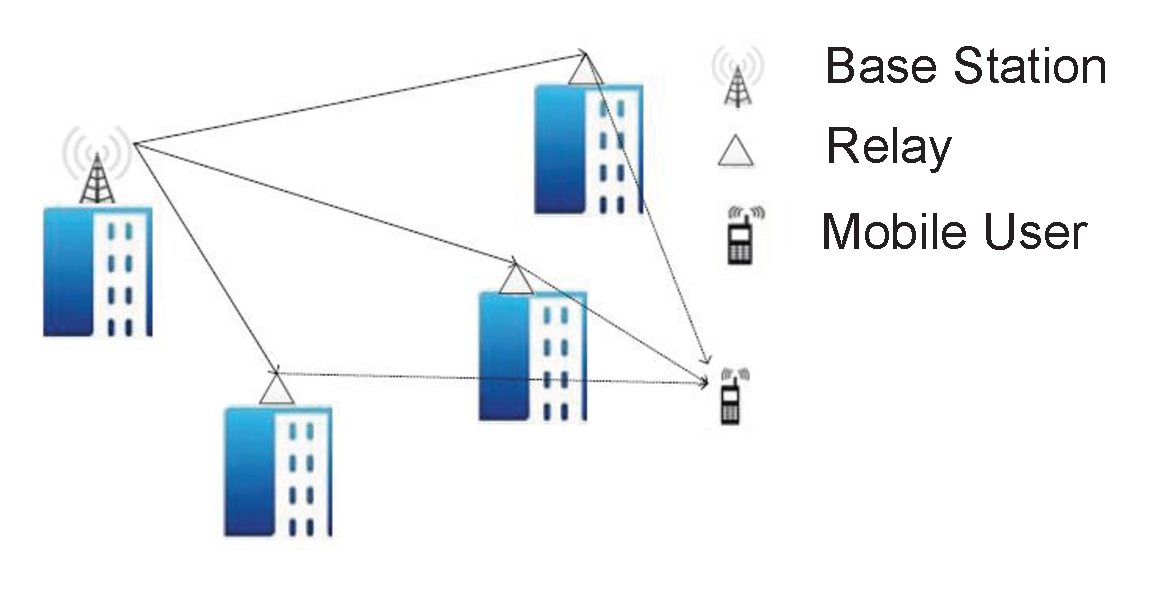
\includegraphics[width=8cm]{buildingversion2.eps}
\caption{Cooperative Communication Example}
\label{building}
\end{figure}
\par Cooperative communication has been proven to be an efficient way to mitigate fast fading and increase the robustness of data connections \cite{chang2009performance,lee2009performance}. However, cooperative communication can also efficiently maintain the connection whenever the channel condition experiences a sudden deterioration due to shadow fading by switching to different relays. Figure \ref{building} is an example of cooperative communication where relays and BS are placed on the top of buildings. In this case, when the MS moves to the area behind a tall building, with a high probability the signal transmitted from the BS will be obstructed by the building, and consequently the MS will encounter deep shadow fading. The channel  between BS and MS will degrade and data rate will drop suddenly. In the worst case scenario, the connection with the BS may be totally lost. To combat this effect and enhance the signal received by the MS in this case, relays can be deployed on the top of tall buildings to relay the signals from the BS to MS to maintain good channel conditions between the BS and MS.
\par Cooperative communication has been a topic of research for several years. Madan et al. \cite{madan2008energy} studied multi-user spatial diversity in a shadow-fading environment. Other work \cite{emamian2002multi,kasiri2008new,park2011opportunistic}, studied relay selection and cooperative relaying over different fading channels in different systems. Patwari et al. \cite{bletsas2006outage} studied relay placement in realistic deployments and confirmed that Rayleigh fading alone is not an appropriate assumption for evaluating network performance in a real deployment. In \cite{zlatanov2011average, kaltakis2009uplink}, the authors analyzed outage probability and its duration with cooperative relaying. In an 4G-LTE network, which is strongly resilient to multipath fading, shadow fading becomes the most important fading factor \cite{rappaport1996wireless}. Given the presence of relays, the channel variation experienced by an MS in an environment with correlated shadow fading is still an open problem. In this chapter, we analyze this problem in a single cell, and give insights on how relays could mitigate shadow fading. We will derive the critical relay density that can guarantee a certain QoS between the BS and an MS.
\par In most cases, shadow fading is modeled as an independent log-normal distribution \cite{goldsmith2005wireless} with a standard deviation derived from empirical measurements. An independent log-normal shadowing model is used widely when shadow fading cannot be ignored. In the log-normal shadowing model, the path loss $\psi$ is assumed random, with a log-normal distribution given by
\begin{equation}
p(\psi)=\frac{\xi}{\sqrt{2\pi}\sigma_{\psi_{dB}}\psi}exp[-\frac{(10\log_{10}\psi-\mu_{\psi_{dB}})^{2}}{2\sigma_{\psi_{dB}}^{2}}], \psi>0,
\end{equation}
where $\xi=10/\ln10$, $\mu_{\psi_{dB}}$ is the mean of $\psi_{dB}=10\log_{10}\psi$ and $\sigma_{\psi_{dB}}$ is the standard deviation of $\psi_{dB}$.
The distribution of the $dB$ value of $\psi$ is Gaussian with mean $\mu_{\psi_{dB}}$, standard deviation $\sigma_{\psi_{dB}}$ and is given by:
\begin{equation}
p(\psi_{dB})=\frac{1}{\sqrt{2\pi}\sigma_{\psi_{dB}}}exp[-\frac{(\psi_{dB}-\mu_{\psi_{dB})^2}}{2\sigma_{\psi_{dB}}^2}].
\end{equation}
The above model fails to capture the spatial correlations in shadow fading. Empirical measurements show that shadowing has significant correlations in realistic scenarios that can affect system performance \cite{graziano1978propagation}. Considering the distribution of obstructions and the speed of the MS, a realistic channel propagation model should incorporate correlated shadow fading.  Szyszkowicz et al. \cite{szyszkowicz2010feasibility} presented a review and analysis of the feasibility of different correlated shadowing models.
\par In cooperative communications, relays help the BS to maintain the connection with the MS. Different cooperative schemes can be used by relays. Typically there are two schemes: Amplify-and-Forward (AF), Decode-and-Forward (DF) \cite{nosratinia2004cooperative}. In the AF mode, relays amplify the noisy signal received from the source and forward to the MS. In the DF mode, relays decode the signal received from the BS, then encode it and forward the coded signals to the MS. In this chapter, we assume that DF scheme is used by relays.
\par Given a fixed placement of BS and a fixed moving trajectory for the MS, the efficient placement of relays to maintain the connection between BS and MS and the resulting reduction of the MS's outage probability under correlated shadow fading is the main focus of this chapter. The key contributions of this chapter are summarized below.
\begin{itemize}
\item An analysis of the relationship between correlated shadow fading and correlated outage events.
\item Show how relays help mitigate correlated shadow fading. Correlated outage fields with and without relaying are given and compared.
\item Analyze the performance of three different relay deployment schemes with different relay densities. The performance includes computing the best channel gain and the resulting change in outage probabilities. We also compare the advantages and disadvantages of different relay deployments.
\end{itemize}
The chapter is organized as follows: Section~\ref{sec:Shadow} presents the correlated shadow fading model that is used in this chapter and the resultant correlated outage. Section~\ref{sec:SystemModel} presents the system model with three different relay deployments. Section~\ref{sec:AA} gives theoretical analysis of how relays mitigate shadow fading and reduce outage probability. Section~\ref{sec:Simulation} presents the simulation setup and analyzes the simulation results of different relay deployments. Section~\ref{sec:Conclusions} summarizes the chapter.
\section{Correlated Shadow Fading}
\label{sec:Shadow}
As stated in the introduction, empirical measurements show that there exist different patterns of correlations between the shadowing. The independent log-normal shadow fading model, while very useful for static MS performance analysis, cannot reflect the correlation of shadow fading between different locations. In this section, we will give a brief introduction of shadow fading models, including the model used in this chapter.
\begin{figure}
\centering
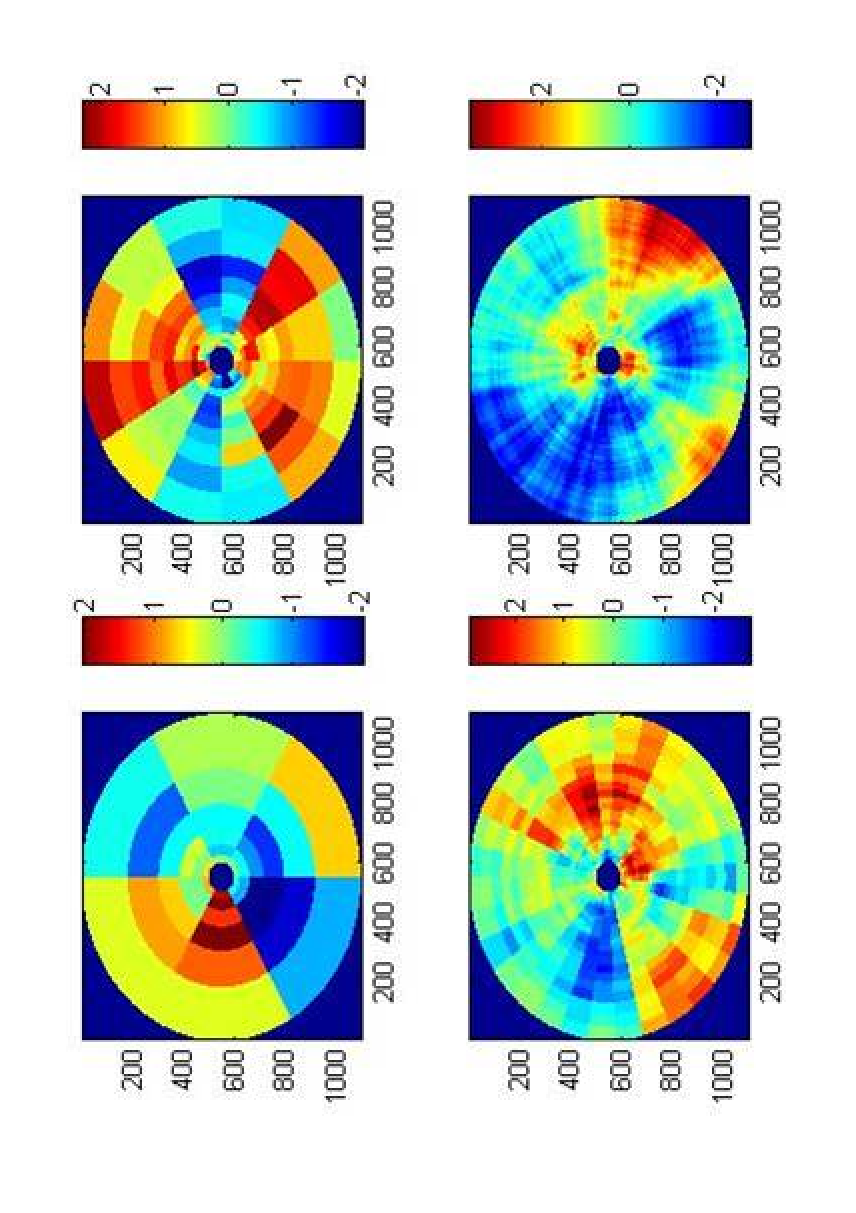
\includegraphics[width=6cm,angle=270]{shadowingfield_V3.eps}
\caption{Correlated Shadowing Fields for Increasing Resolutions (The disk area is the generated correlated shadowing field and the color of the areas refers to the normalized standard deviation which is $S_{i}/\sigma_{s}(\vec{r_{i}})$)}
\label{shadowingfield}
\end{figure}
%In most cases, shadow fading is considered as independent log-normal. But from empirical measurements we can see that there exits different correlations between shadow fading factor.
There is no single mathematical model which captures all different categories of correlation\cite{szyszkowicz2010feasibility}. In this chapter, we use the correlated shadow fading model which incorporates the angular and distance correlations of shadow fading \cite{szyszkowicz2011interference}. In \cite{szyszkowicz2011interference}, the author states that correlation in shadowing is indispensable for the analysis of interference of large networks and gives a time-efficient fast shadowing fields generation algorithm. The algorithm generates a correlated shadowing field $\vec{S}$, which gives shadow fading factor $\vec{s_{i}}$ for each path $\vec{r_{i}}$ with a correlation matrix
\begin{equation}
\mathbf{K}_{N\times N} = [ \sigma_{s}(\vec{r_{i}})\sigma_{s}(\vec{r_{j}})h(\vec{r_{i}}\vec{r_{j}})],
\label{correlationmatrix}
\end{equation}
where $N$ paths interfere with path $\vec{r_{i}}$ and $\mathbf{E}\{S_{i}^{2}|\vec{r_{i}}\}=\sigma_{s}^{2}(\vec{r_{i}})$. This model assumes that in the correlation matrix, $h$ is separable with respect to the angle of arrival
\begin{equation}
\theta = |\angle\vec{r_{i}}-\angle\vec{r_{j}}|\in [0^{\circ},180^{\circ}],
\end{equation}
and the arrival distance ratio
\begin{equation}
R=|10\log_{10}r_{i}/r_{j}|=\frac{10}{\ln 10}|\ln r_{i}-\ln r_{j}|,
\end{equation}
\begin{equation}
h(\vec{r_{i}},\vec{r_{j}})=max\{1-\theta/\theta_{0},0\}\cdot max\{1-R/R_{0},0\}.
\end{equation}
Following the fast shadowing field generation algorithm, we generate shadowing fields with different values of tuneable parameters. The shadowing fields are shown in Figure \ref{shadowingfield} with increasing resolutions. Four circular correlated shadowing fields are generated.
The shadowing fields are similar to those generated in \cite{szyszkowicz2011interference}.
\subsection{Correlated Outage Field}
\label{outagefield}
\begin{figure}
\centering
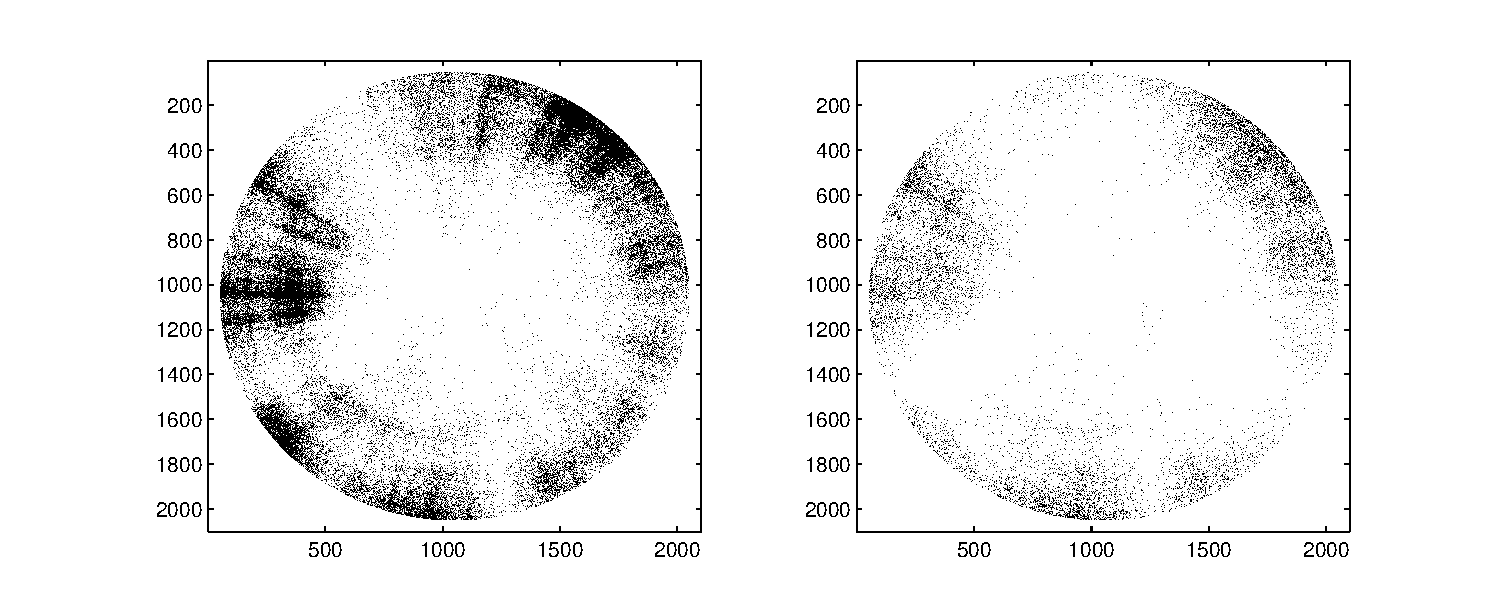
\includegraphics[width=12cm]{outagefield.eps}
\caption{Correlated Outage Fields (Dark areas are outage areas while white areas are non-outage areas)}
\label{outagefie}
\end{figure}
Given a correlated shadowing field, the outage events at different locations are also correlated. Here we analyze correlated outage events under correlated shadow fading and later give an example. In the spatial correlation of outage events, without considering Rayleigh fading, path loss is considered as constant at a fixed time point. Based on the correlated shadowing field we can generate a correlated outage field. Let $G$ denotes total channel gain, $PL$ denotes path loss, %$R$ denote the norm of small-scale Rayleigh fading factor,
and $S$ denotes shadow fading factor, we then have:
\begin{equation}
G = PL* S
\end{equation}
For two different positions, the correlation coefficient of the two total channel gains is of the following form:
\begin{equation}
\rho_{1,2} = \frac{E[G_{1}G_{2}]}{\sqrt{(Var(G_{1})Var(G_{2}))}}.
\label{eq1}
\end{equation}
where $G_{1}=PL_{1}*S_{1}$ and $G_{2}=PL_{2}*S_{2}$.
At a fixed time point, temporal correlation is neglected and only spatial correlation is considered, then $PL_{1}$, $PL_{2}$ can be assumed to be constants, which means that $E[PL_{1}] = PL_{1}$, $E[PL_{2}] = PL_{2}$. Based on this assumption, we have
\begin{equation}
E[G_{1}G_{2}] = PL_{1}PL_{2}E[S_{1}S_{2}],
\label{eq2}
\end{equation}
\begin{equation}
Var(G_{1}) = PL_{1}^{2}Var(S_{1}),
\label{eq3}
\end{equation}
\begin{equation}
Var(G_{2}) = PL_{2}^{2}Var(S_{2}),
\label{eq4}
\end{equation}
Based on \eqref{eq2}, \eqref{eq3} and \eqref{eq4}, it is straightforward to rewrite \eqref{eq1} as:
\begin{equation}
\rho_{1,2} = \frac{E[S_{1}S_{2}]}{\sqrt{Var(S_{1})Var(S_{2})}} = \rho_{S_{1},S_{2}}.
\end{equation}
The channel gain has a spatial correlation coefficient as shown above. Based on the result above, a correlated channel gain field can be generated. Given a proper threshold $\gamma$, the correlated outage field can be generated as in Figure \ref{outagefie}. On the left, a correlated outage field without relaying is shown while the correlated outage field with relaying (3 relays uniformly placed on a circle near the edge) is given on the right. The black color indicates outage areas. In the next section we will present the methodology that helped us generate the results with relays.

\begin{figure}
\centering
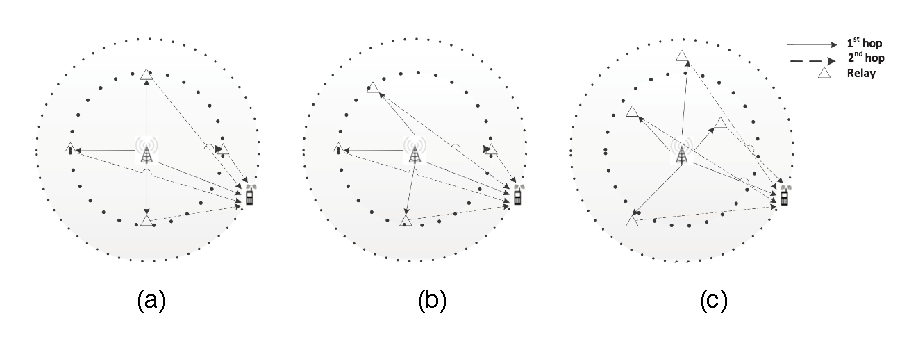
\includegraphics[width=14cm]{abc.eps}
\caption{System Model and Three Different Relay Placements}
\label{threemodels}
\end{figure}
\section{System Model}
\label{sec:SystemModel}
Since most of the key aspects of the problem can be studied in a single cell, we consider a single cell cellular deployment, where the BS is located at the center of the cell.  Figure \ref{threemodels} shows the system model that is used in this chapter. Several relays are placed in the cell and an MS is moving at a particular speed along the circumference at the cell edge. We picked this trajectory since it is the most challenging path given the combination of shadowing and path loss. We consider three relay deployment modes. From left to right in Figure \ref{threemodels}, (a) is the mode where relays are placed uniformly on a circle near the cell edge; (b) is relays that are randomly spaced on a circle near the cell edge; (c) is relays placed randomly in the cell. By varying relay densities in the above three different models we can analyze which combination of relay density and relay placement can meet the required QoS.

\subsection{Cooperative Communication Scheme}
\label{Towhop}
\par In this system, the BS and relays work cooperatively to try to guarantee that the MS has sufficient received power either from the BS or from relays with high probability. There are two main cooperative communication schemes: Amplify-and-Forward, and Decode-and-Forward. In this chapter, we assume that relays use the Decode-and-Forward scheme. The cooperative communication system works in the following manner:
\begin{itemize}
\item First Hop: BS broadcasts signals to both relays and MS. If MS receives and decodes the signals transmitted by the BS successfully, there is no need for relays to repeat the transmission. If not, relays which successfully decode the signals will participate in the second hop retransmission. This mode of operation will require some signaling overhead, which is not addressed in this chapter. Relays which cannot decode the received signal successfully, will not participate in the second hop.
\item Second Hop: Among all relays which participate in the second hop, the one that has the best channel gain between the relay and MS will be chosen (this can be done by centralized control or using information from pilot signals). This relay will encode the signals again and send the coded bits to the MS.
\end{itemize}

\par The received signal in a link $(S\to D)$ between the source and destination is given by:
\begin{equation}
y_{D} = G_{SD}x_{S}+n_{D}.
\end{equation}
where $x_{S}$ is the signal transmitted by the source and $y_{D}$ is the signal received by the destination. $n_{D}\sim \mathcal{CN}(0,N_{0})$ is additive white Gaussian noise. $G_{SD}$ is the channel gain from source to destination including path loss and shadow fading. $\text{SNR} \triangleq P*G_{SD}^{2}/N_{0}$, is the end-to-end received signal-to-noise ratio (SNR) and $P$ is the transmitted power. The destination successfully receives the signals if no outage event happens, i.e., $\log_{2}(1+\text{SNR})\ge R$, where $R$ is the required data rate. From the definition of SNR, no outage event happens as long as SNR $> \gamma$, where $\gamma = 2^{R}-1$.
In the first hop, relays that can successfully decode the signals transmitted from the BS is a subset $\mathcal{R}_{n}$ of $N$ relays defined by:
\begin{equation}
\mathcal{R}_{n}\triangleq \{ i: \log_{2}(1+\text{SNR}_{S-i})\ge R\},
\end{equation}
where $\text{SNR}_{S-i}$ is the received signal-to-noise ratio from BS to relay $i$ and $n\in\{0,1,\cdots,2^{N}\}$.
%The channel gain of the source-relay channel is denoted by $X_{i}$ for the $i$th relay where $i\in {1,2,\cdots,N}$, where $N$ is the total number of relays.
In the first hop, the relay can successfully decode the BS signals if $\text{SNR}_{S-i}>\gamma$. The indices of all relays which are able to successfully decode BS signals form a set $\mathcal{R}_{n}$. In the second hop, the selected best relay $j$ is the relay in $\mathcal{R}_{n}$ that has the maximum SNR among all relays in $\mathcal{R}_{n}$, i.e., $j=\arg\max_{i\in \mathcal{R}_{n}}\{\text{SNR}_{i-D}\}$, where $\text{SNR}_{i-D}$ denotes the SNR from the $i$th relay to the destination MS. The BS to MS SNR is denoted by $\text{SNR}_{S-D}$. The SNR is determined by distance related path loss and large-scale correlated shadow fading.

\section{Outage Probability Analysis}
\label{sec:AA}
Due to the variations of the channel gain caused by shadow fading and path loss of the propagation environment, if the  end-to-end  channel capacity is below the transmission rate, an outage occurs and the information packets are lost. The outage probability is an important performance measurement of the communication system. In this section, the expression for outage probability is derived.

\subsection{Outage Probability of the Cooperative Communication System}
\label{outageprobability}
 If an MS cannot directly receive the signal from the BS and none of the relays can decode the BS signal, or if the MS has a bad channel with all relays which successfully decode the BS signal, then an outage event will take place. The probability that an MS cannot receive signals directly from the BS successfully is given below:
\begin{equation}
P_{out_{0}} = P[\text{SNR}_{S-D}<\gamma],
\end{equation}
Under the assumption that an MS cannot successfully receive signals from the BS, the outage event happens in the first hop if no relay can receive the signal from the BS successfully, which means $\mathcal{R}_{0}=\phi$. Based on this assumption we have:
\begin{equation}
P_{out_{1}} = \max_{i = 1,\cdots,N} P[\text{SNR}_{S-i}<\gamma].
\end{equation}
If the outage does not happen in the first hop, then the outage event may happen in the second hop with probability:
\begin{equation}
P_{out_{2}} = \sum_{n=1,\cdots,2^{N}}P[\text{SNR}_{j-D}<\gamma|\mathcal{R}_{n}]P[\mathcal{R}_{n}],
\end{equation}
where $j$ is the index of the relay which has the best channel gain between it and the MS.
So the outage probability of the system is
\begin{equation}
P_{out_{S}} = P_{out_{0}}*(P_{out_{1}}+(1-P_{out_{1}})*P_{out_{2}}).
\end{equation}
The probability density function (pdf) of shadow fading $S$ given $L$ correlated fading branches is
\begin{equation}
\begin{split}
f_{\mathbf{S}}(\mathbf{s}) = &\frac{\lambda^{L}}{\sqrt{2\pi}|\mathbf{K}_{L\times L}|^{1/2}\prod_{i=1}^{L}s_{i}}\\
&\cdot\exp(-\frac{1}{2}(10\log_{10}\mathbf{s}-\boldsymbol{\mu})^{T}\mathbf{K}_{L\times L}^{-1}(10\log_{10}\mathbf{s}-\boldsymbol{\mu})),
\end{split}
\end{equation}
where $\lambda = 10/\ln10$ and $\boldsymbol{\mu}$ is the average shadow fading which is normally $0$. $\mathbf{K}_{L\times L}$ is the correlation matrix which is defined in \eqref{correlationmatrix}. Let $\theta_{i} = \frac{10\log_{10}s_{i}-\mu_{i}}{\sqrt{2}\sigma_{i}}$, and doing a change of variables gives us the pdf of $\mathbf{\Theta}$ as follows:
\begin{equation}
f_{\mathbf{\Theta}}(\mathbf{\theta}) = \frac{1}{\pi^(L/2)|\mathbf{\Sigma}|^{1/2}}\exp(-\mathbf{\Theta}^{T}\mathbf{\Sigma}^{-1}\mathbf{\Theta}),
\end{equation}
where $\mathbf{\Sigma}$ is the correlation coefficient matrix which is
\begin{equation}
\left[\begin{array}{cccc}
1 & h_{1,2} & \cdots & h_{1,L}\\
\vdots & \ddots & \ddots & \vdots\\
h_{L,1} & h_{L,2} & \cdots & 1\\
\end{array}\right].
\end{equation}
Since SNR$=PL+S-N_{0}$ in dB, SNR$>\gamma$ means $S>\gamma-PL+N_{0}$.
%Without loss of generality, we assume Rayleigh fading has average power $1$. To guarantee $99.9\%$ average successfully transmission, $R_{th}=-7dB$. So shadow fading threshold is $\gamma>\beta-PL+7dB+N_{0}$.
Given $\mathcal{S}_{0}=\phi$, and letting $\gamma_{ai}$ denote the shadow fading threshold for the $i$th relay in the $a$th hop and where $a=0,1,2$, where the $0$th hop is the direct transmission from BS to MS, we then have
\begin{equation}
P_{out_{1}} = \underbrace{\int_{-\infty}^{+\infty}\cdots\int_{-\infty}^{+\infty}}_{i =1,\cdots,N}\prod g_{0}(\gamma_{1i})f(\mathbf{s_{1}})d\mathbf{s_{1}}.
\end{equation}
For $n=1,\cdots,2^{N}$, the outage probability for the second hop is
\begin{equation}
\begin{split}
P_{out_{2}} = \sum_{n=1,\cdots,2^{N}}\underbrace{\int_{-\infty}^{+\infty}\cdots\int_{-\infty}^{+\infty}}_{i=1,\cdots,N}\prod g_{n}(\gamma_{1i}) f(\mathbf{s_{1}})d\mathbf{s_{1}}\\
\cdot\underbrace{\int_{-\infty}^{+\infty}\cdots\int_{-\infty}^{+\infty}}_{i\in \mathcal{R}_{n}}\prod g_{n}(\gamma_{2i})f(\mathbf{s_{2}})d\mathbf{s_{2}},
\end{split}
\end{equation}
where $\mathbf{s_{1}}$ is the correlated shadow fading in the first hop, $\mathbf{s_{2}}$ is the correlated shadow fading in the second hop, $u$ is a step function and
\begin{equation}
g_{n}(\gamma_{ai}) = \{\begin{array}{cc}
               u(\gamma_{ai}) & i\in \mathcal{R}_{n} \\
               1-u(\gamma_{ai}) & i\notin \mathcal{R}_{n}
             \end{array}.
\end{equation}
Due to the random nature of propagation environment, $P_{out_{0}}$ is beyond our control. Therefore, to reduce the outage probability, we need to reduce $P_{out_{1}}$ and $P_{out_{2}}$. Relays at proper positions with sufficient density can reduce the outage probability. Comparing different relay placements and finding the appropriate relay density to guarantee the outage probability requirement is the main issue that we will consider next.

%\par Considering a simple case where we have two relays which are far away from each other (no shadow fading correlation) and all shadow fading factor have the same average $\mu$ and standard deviation $\sigma$, the outage probability is given as:
%\begin{equation}
%P_{out_{0}}=\int_{-\infty}^{\gamma_{00}}f(\mathbf{s})d\mathbf{s}=\Phi(\frac{\gamma_{00}-\mu}{\sigma})
%\end{equation}
%\begin{equation}
%P_{out_{1}}=\int_{-\infty}^{\gamma_{11}}\int_{-\infty}^{\gamma_{12}}f(\mathbf{s1})d\mathbf{s1}=\Phi(\frac{\gamma_{11}-\mu}{\sigma})\Phi(\frac{\gamma_{12}-\mu}{\sigma})
%\end{equation}
%\begin{equation}
%\begin{split}
%P_{out_{2}}=\int_{\gamma_{11}}^{+\infty}\int_{\gamma_{12}}^{+\infty}f(\mathbf{s1})d\mathbf{s1}\int_{-\infty}^{\gamma_{21}}\int_{-\infty}^{\gamma_{22}}f(\mathbf{s2})d\mathbf{s2}\\
%+\int_{\gamma_{11}}^{+\infty}\int_{-\infty}^{\gamma_{12}}f(\mathbf{s1})d\mathbf{s1}\int_{-\infty}^{\gamma_{21}}\int_{-\infty}^{+\infty}f(\mathbf{s2})d\mathbf{s2}\\
%+\int_{-\infty}^{\gamma_{11}}\int_{\gamma_{12}}^{+\infty}f(\mathbf{s1})d\mathbf{s1}\int_{-\infty}^{+\infty}\int_{-\infty}^{\gamma_{22}}f(\mathbf{s2})d\mathbf{s2}\\
%=[1-\Phi(\frac{\gamma_{11}-\mu}{\sigma})][1-\Phi(\frac{\gamma_{12}-\mu}{\sigma})]\Phi(\frac{\gamma_{21}-\mu}{\sigma})\Phi(\frac{\gamma_{22}-\mu}{\sigma})\\
%+[1-\Phi(\frac{\gamma_{11}-\mu}{\sigma})]\Phi(\frac{\gamma_{12}-\mu}{\sigma})\Phi(\frac{\gamma_{21}-\mu}{\sigma})\\
%+[1-\Phi(\frac{\gamma_{12}-\mu}{\sigma})]\Phi(\frac{\gamma_{11}-\mu}{\sigma})\Phi(\frac{\gamma_{22}-\mu}{\sigma})
%\end{split}
%\end{equation}
%where $\Phi$ is the cumulative distribution function (CDF) of the standard normal distribution. For complicated case with correlated shadow fading, numerical analysis can be done and it will give us an idea of how relays can help mitigate correlated shadow fading.
\section{Simulation and Performance Evaluation}
\label{sec:Simulation}
To study which relay placement yields the best system performance i.e., the lowest outage probability for continuous real-time applications that we assume to be running on an MS moving at the cell edge (for the given cooperative communication scheme), we set up simulations and compare performance for different relay placements.
\subsection{Relay Placement}
Different relay placements as shown in Figure \ref{threemodels} are studied and compared in this section.
\begin{itemize}
\item Mode 1: Relays are uniformly spaced on a circle near the cell edge.
    \item Mode 2: Relays are randomly spaced on a circle near the cell edge.
    \item Mode 3: Relays are randomly placed in the cell.
    \end{itemize}
%\subsection{Correlated Shadowing Fields}
%\begin{figure*}
%\centering
%\subfigure[First Hop]{
%\includegraphics[width=4.5cm]{hop1.eps}
%\label{hop1}}
%\hfil
%%\subfigure[Second Hop]{
%%\includegraphics[width = 2.3in,trim= .12in  .73in .62in .4in, clip]{hop1tohop2version2.eps}
%%\caption{TDD half duplex baseline and dull duplex operation.}
%%\label{hop2}
%\subfigure[Second Hop]{
%\includegraphics[width=11cm]{hop1tohop2version33.eps}
%\label{hop2}
%}
%\caption{First Hop and Second Hop Correlated Shadowing Fields. Spatial correlation is demonstrated in the second hop. When MS moves from position A to position B which is one de-correlation distance away from A, a new correlated shadowing field is generated and applied. As we have stated, the cross-correlated shadowing factors associated with links from different relays to the MS can be considered as the auto-correlated shadowing factors associated with the links from MS to different relays.}
%\label{fig4}
%\end{figure*}
%Here, a spatially-correlated shadowing field is generated to reflect the shadow fading factor. Figure \ref{fig4} gives an example of the correlated shadow fading field in the two hop transmission. The shadowing field is coarser than the real one used in the simulation in order to simply and clearly demonstrate the correlated feature of shadow fading. In the first hop, a correlated shadowing field is generated with the BS at the center of the field and with a fixed shadow fading factor corresponding to every relay and every MS position. In the second hop, a correlated shadowing field is generated with the MS at the center of the field. According to \cite{yamamoto2006impact} and \cite{lopez2007resiliency}, auto-correlation and cross-correlation of two interfering paths are very similar and can be studied in the same frame work. Here in our case,
%%the symmetric character between cross-correlation and auto-correlation,
%the cross-correlation of the shadow fading of the links from different relays to MS can be considered as the auto-correlation of the shadow fading of the links from the MS to different relays.
%So only one correlated shadowing field needs to be generated. In both of the two hops, the time-correlation is assumed to be $1$ within $D_{decor}/v$, where $v$ is the speed of the MS and $D_{decor}$ is the de-correlation distance. So an independent correlated shadowing field is generated at every de-correlation distance as shown in Figure \ref{fig4}.

\subsection{Simulation Configuration}
In this chapter, the Okumura-Hata model \cite{saunders2007antennas} is used to estimate the path loss.
%The path loss is
%\begin{align}
%PL_{dB} &= A + B\log_{10}R - E\\
%\text{where } A &= 69.55 + 26.16\log_{10}f - 13.82\log_{10}h_{b}\\
%B &= 44.9 - 6.55\log_{10}h_{b}\\
%E &= 3.2(\log_{10}(11.7554h_{m}))^{2} - 4.97
%\end{align}
%where $R$ is the distance from source to destination[$km$], $h_{m}$ is the destination antenna height above local terrain %height[$m$], $h_{b}$ is the source antenna height above local terrain height[$m$].
%It is assumed that the system undergoes Rayleigh fading, which is small-scale fading in addition to shadow fading.
The values of parameters that are used in the simulation are shown in Table \ref{SystemConfig}. In Mode 1 and Mode 2, the radius of the circle where relays are placed (near the edge) is $700m$.
\begin{table}
\centering
\caption{\label{SystemConfig}Simulation Configuration Parameters}

\begin{tabular}{|c|c|}

\hline

\multirow{3}{*}{Okumura-Hata Model} & BS Height: $100m$\\
& Relay Height: $10m$\\
& MS Height: $1.5m$\\
\hline
%Rayleigh Fading & Coherence Time: $100ms$\\
%\hline
\multirow{4}{*}{Correlated Shadow Fading} & $R_{0}: 6$\\
& $\theta_{0}: \pi /3$\\
& $d_{min}: 50m$\\
\hline
\multirow{2}{*}{Relay Placements} & Three Modes with Density:\\
& 2,4,6,8,10,12\\
\hline
Cell Size & $R: 1000m$\\
\hline
MS Moving Speed & $v: 10m/s$\\
\hline
Radio Frequency & $f: 900MHz$\\
\hline
BS Transmission Power & $P: 26dbm$\\
\hline
SNR Requirement & $8dB$\\
\hline
\end{tabular}

\end{table}

\subsection{Simulation Results and Analysis}
\begin{figure}
\centering
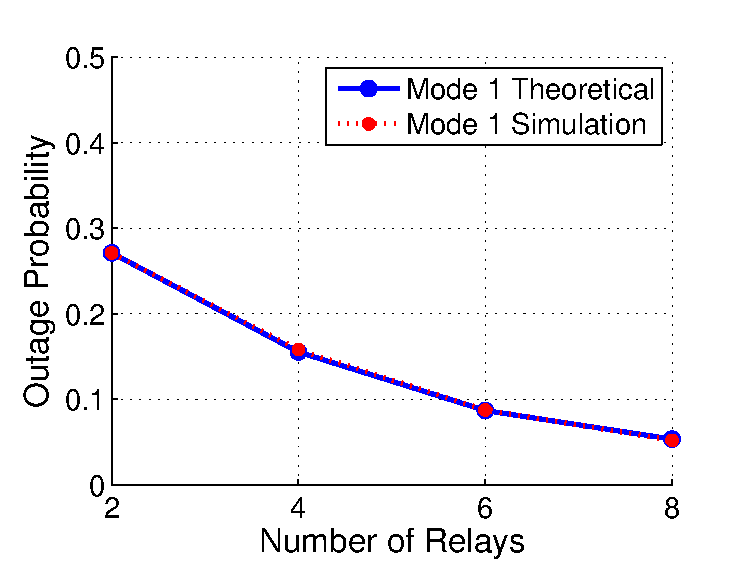
\includegraphics[width=12cm]{theo_vs_simu_V2.eps}
\caption{Theoretical and Simulated Outage Probability for Mode 1}
\label{theovssimu}
\end{figure}

\begin{figure}
\centering
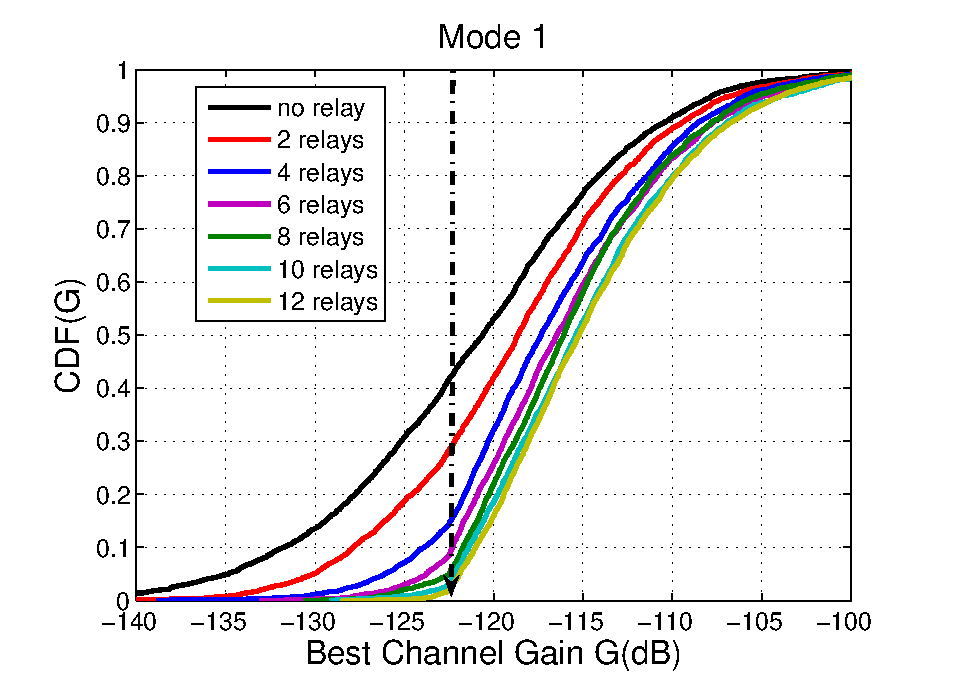
\includegraphics[width=12cm]{Mode1_bestchannelgain_V2.eps}
\caption{Best Channel Condition between MS and BS or Relays of Mode 1 (Dashed arrow demonstrates the channel condition that satisfies the SNR requirement.}
\label{Mode1}
\end{figure}
\begin{figure}
\centering
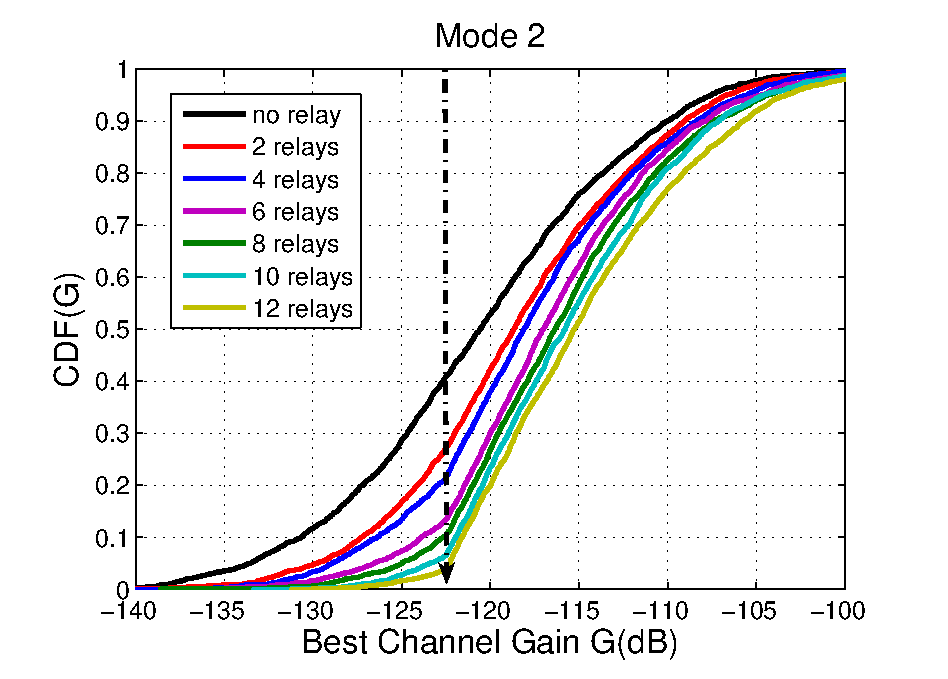
\includegraphics[width=12cm]{Mode2_bestchannelgain_V2.eps}
\caption{Best Channel Condition between MS and BS or Relays of Mode 2 (Dashed arrow demonstrates the channel condition that satisfies the SNR requirement.}
\label{Mode2}
\end{figure}
\begin{figure}
\centering
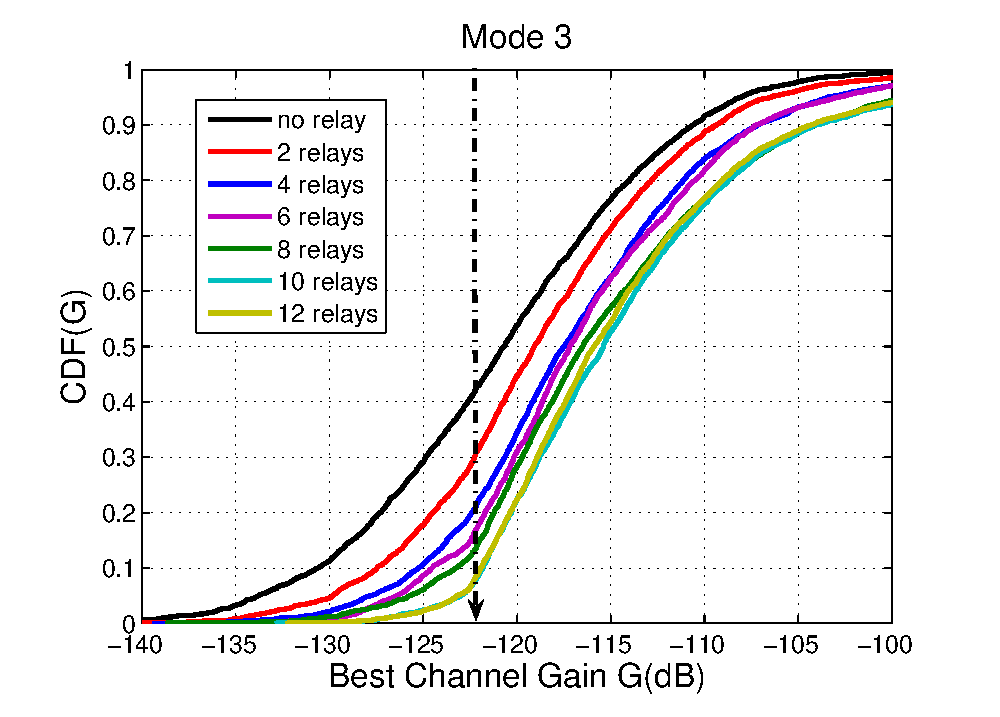
\includegraphics[width=12cm]{Mode3_bestchannelgain_V2.eps}
\caption{Best Channel Condition between MS and BS or Relays of Mode 3 (Dashed arrow demonstrates the channel condition that satisfies the SNR requirement.}
\label{Mode3}
\end{figure}
%\caption{Best Channel Condition between MS and BS or Relays (Dashed arrow demonstrates the channel condition that satisfies the SNR requirement.}
%\label{bestchannelgain}
%\end{figure*}
\begin{figure}
\centering
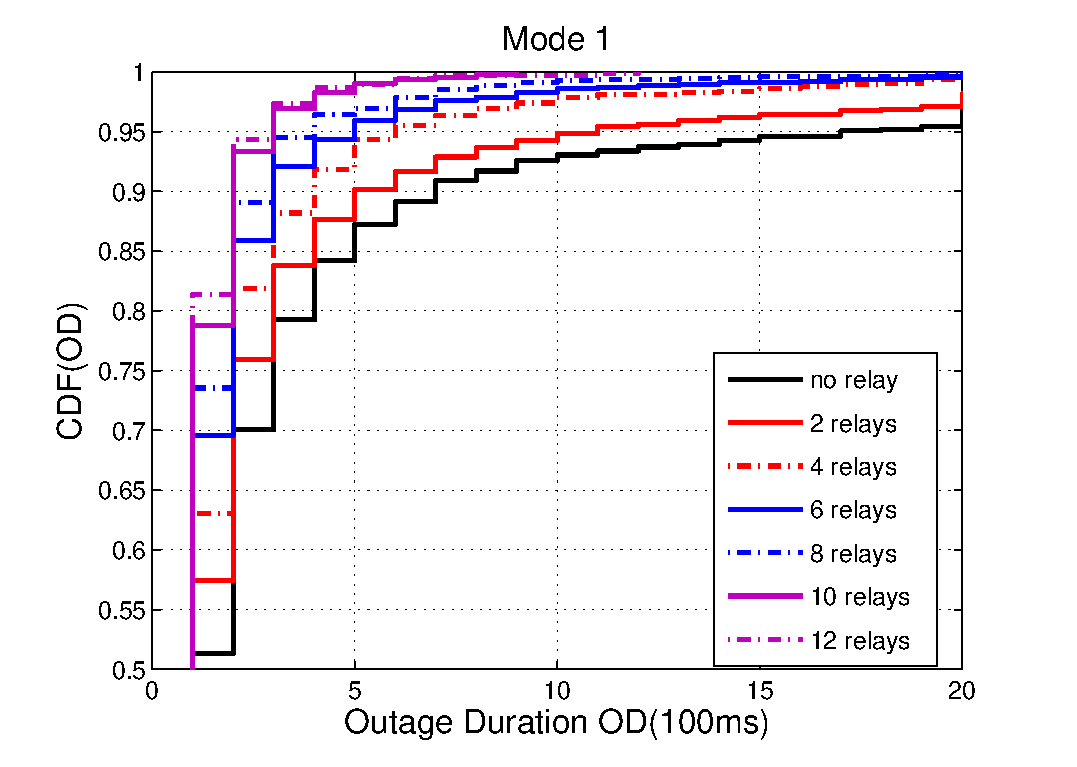
\includegraphics[width=12cm]{OutageDuration_Rayleigh_Mode1_V2.eps}
\caption{Cumulative Distribution Function of Outage Duration of Mode 1 (with Rayleigh fading)}
\label{Mode1Out}
\end{figure}
\begin{figure}
\centering
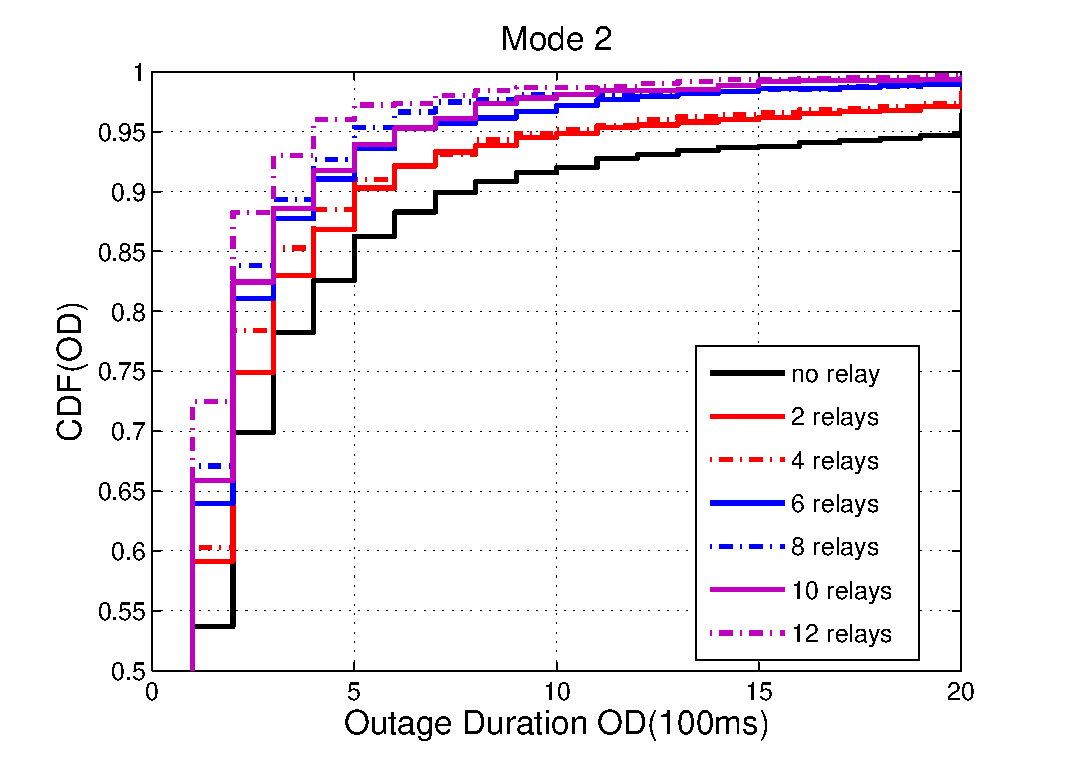
\includegraphics[width=12cm]{OutageDuration_Rayleigh_Mode2_V2.eps}
\caption{Cumulative Distribution Function of Outage Duration of Mode 2 (with Rayleigh fading)}
\label{Mode2Out}
\end{figure}
\begin{figure}
\centering
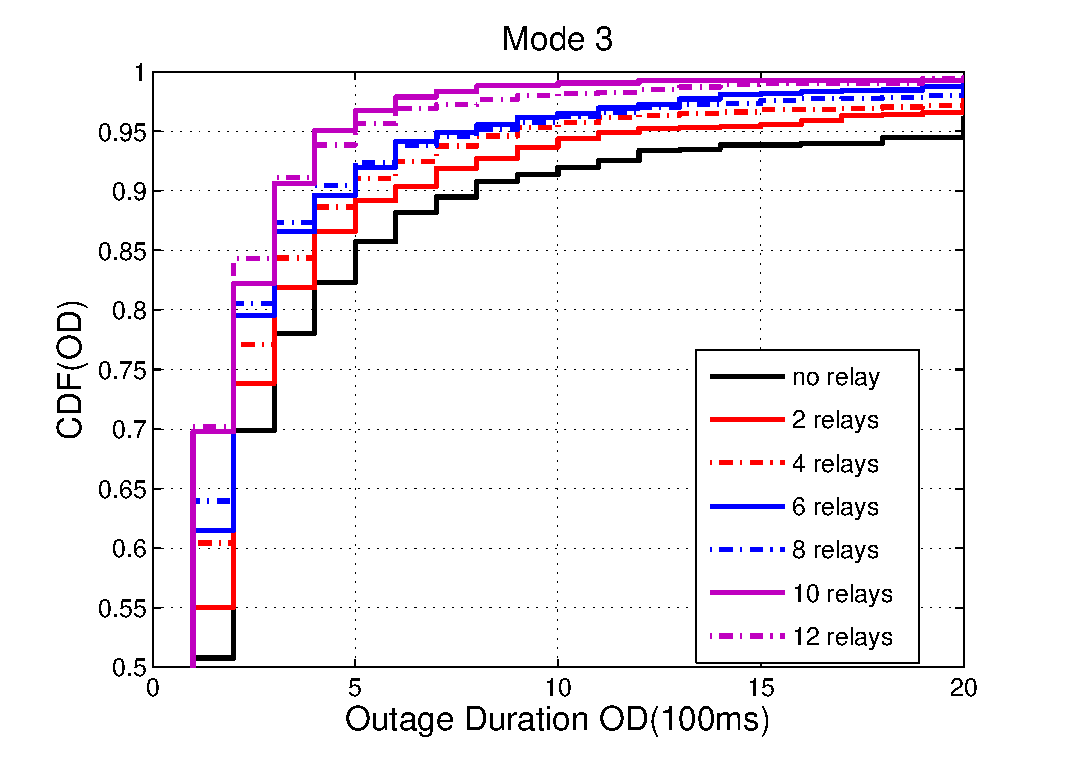
\includegraphics[width=12cm]{OutageDuration_Rayleigh_Mode3_V2.eps}
\caption{Cumulative Distribution Function of Outage Duration of Mode 3 (with Rayleigh fading)}
\label{Mode3Out}
\end{figure}
%\begin{figure*}
%\centering
%\subfigure[Mode 1]{
%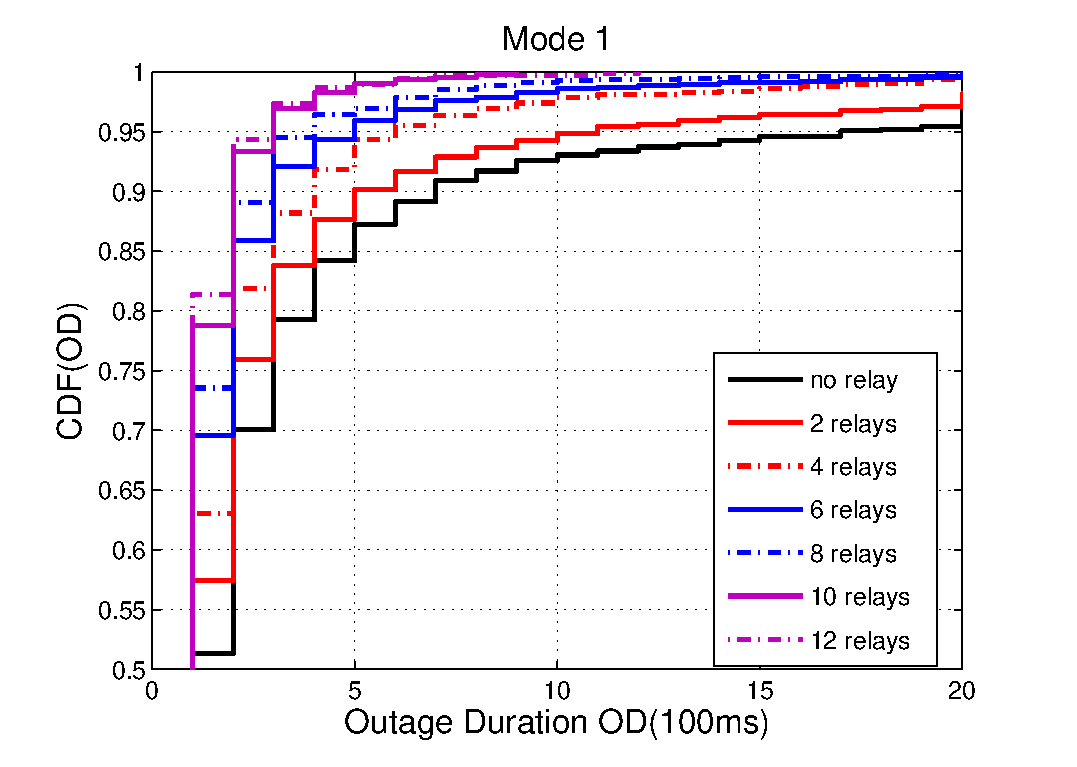
\includegraphics[width=5.5cm]{OutageDuration_Rayleigh_Mode1_V2.eps}
%\label{Mode1}}
%\hfil
%\subfigure[Mode 2]{
%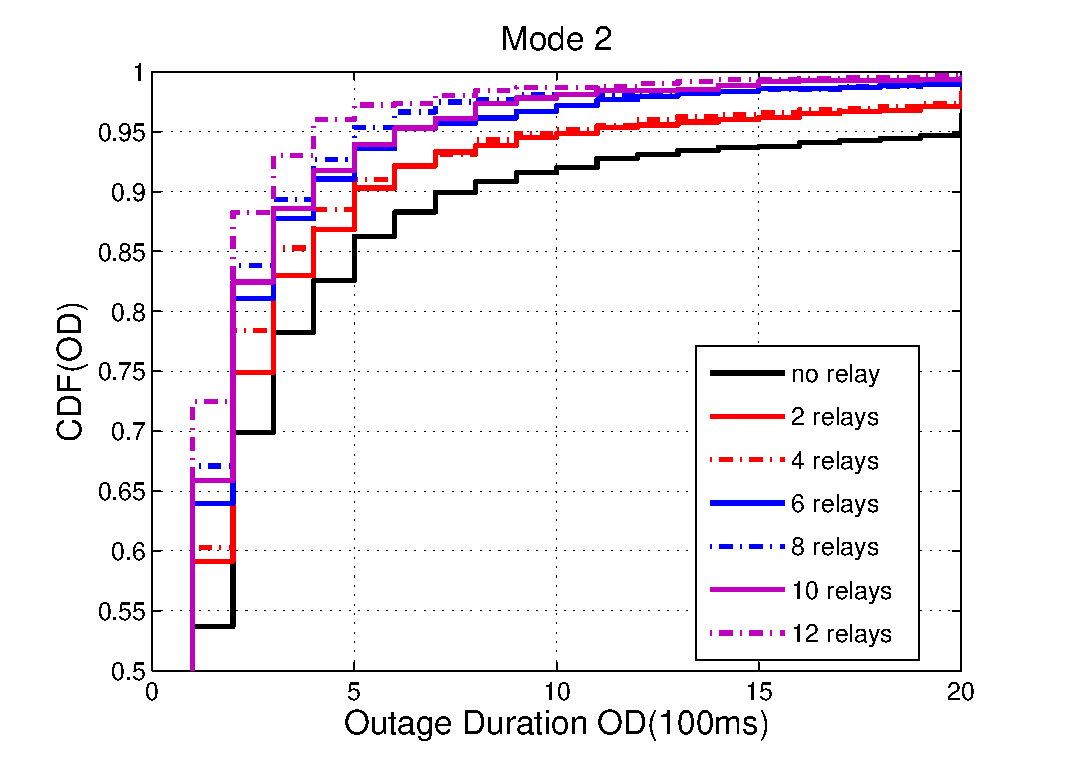
\includegraphics[width=5.5cm]{OutageDuration_Rayleigh_Mode2_V2.eps}
%\label{Mode2}}
%\hfil
%\subfigure[Mode 3]{
%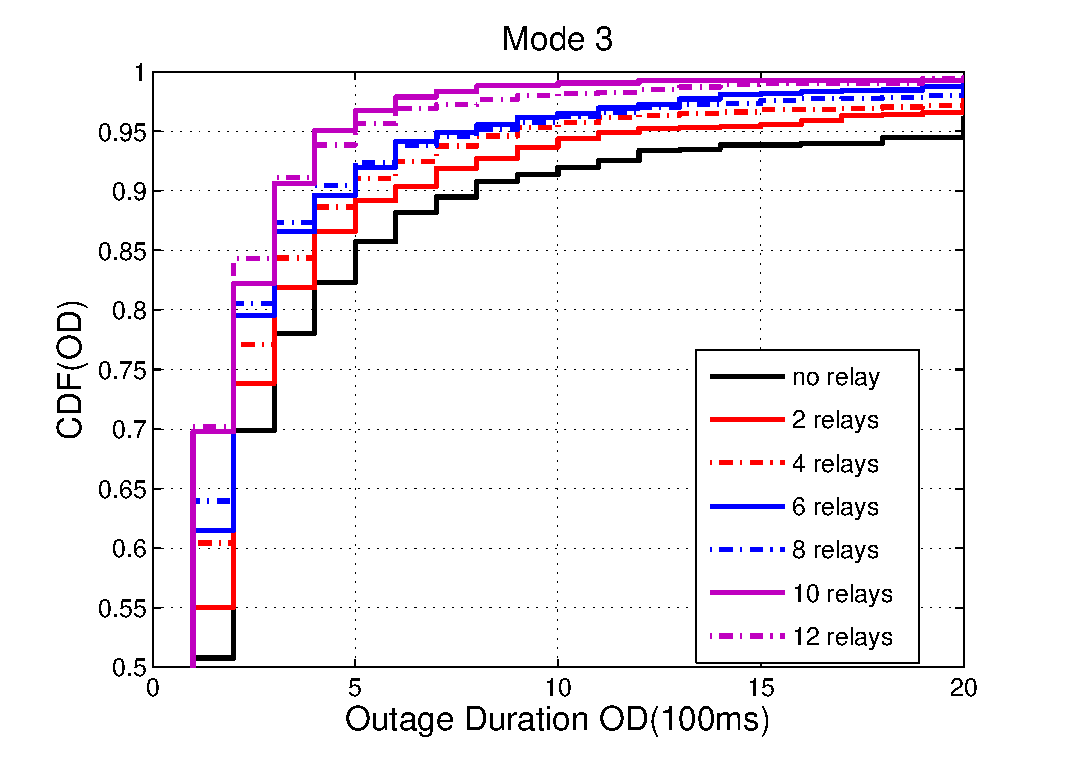
\includegraphics[width=5.5cm]{OutageDuration_Rayleigh_Mode3_V2.eps}
%\label{Mode3}}
%\caption{Cumulative Distribution Function of Outage Duration (with Rayleigh fading)}
%\label{outageperformance}
%\end{figure*}

\par In this section, numerical analysis and simulation results are presented. The best channel condition that the user can get from either BS or relay is simulated to demonstrate the improvement of the received signal strength at the MS. The outage probabilities and durations are shown to indicate the potential user experience improvement when using a real-time application.
\par First, numerical analysis and simulation results of outage probabilities in Mode 1 is shown in Figure \ref{theovssimu}. The numerical analysis has high computational complexity and is difficult to apply to outage duration analysis. Therefore a simulation is necessary to study the system. Considering the computational complexity, to show that our simulation is validated by analysis, partial comparison between numerical analysis and simulation results is shown in Figure \ref{theovssimu}, which indicates that our simulation code is correct and can be used to study the system.
\par Second, we simulate the distribution of the best channel gain for the channel between the MS and BS or relays. Figure \ref{Mode1}, \ref{Mode2}  and \ref{Mode3} plot the distribution of the user channel gain of the three different relay deployment modes and 6 different relay densities. As shown in the figure, the intersection of the dashed arrow and the cumulative distribution function (cdf) plots indicates that as relay density increases, the percentage of outages reduces. The dashed arrow points to $122.5dB$ which is the lowest channel gain to guarantee the SNR to be above $8dB$, in which case 16-QAM with $1/2$ code rate will still work. Considering the power constraints, the complexity and cost of placing relays and received SNR requirements, finding a proper relay density is very important. Beyond a certain relay density, increasing the relay density will not give significant additional performance improvement. In all modes, it is shown that relays can mitigate the shadow fading efficiently. For example, in the Mode 1 case, $10$ relays can improve the performance by reducing the probability of outage by $40\%$ compared to the no relay case. To compare the results across the three different modes, we take the 10 relay case as an example. For this case, Mode 1 has an outage probability $3\%$ less than Mode 2 and $10\%$ less than Mode 3. In addition, we compare the three different modes from the outage frequency point of view. Outage frequency is defined as
\begin{equation}
f_{outage}=\frac{\text{Total Number of Outage Points}}{\text{Total Number of Simulation Points}}.
\end{equation}
\begin{figure}
\centering
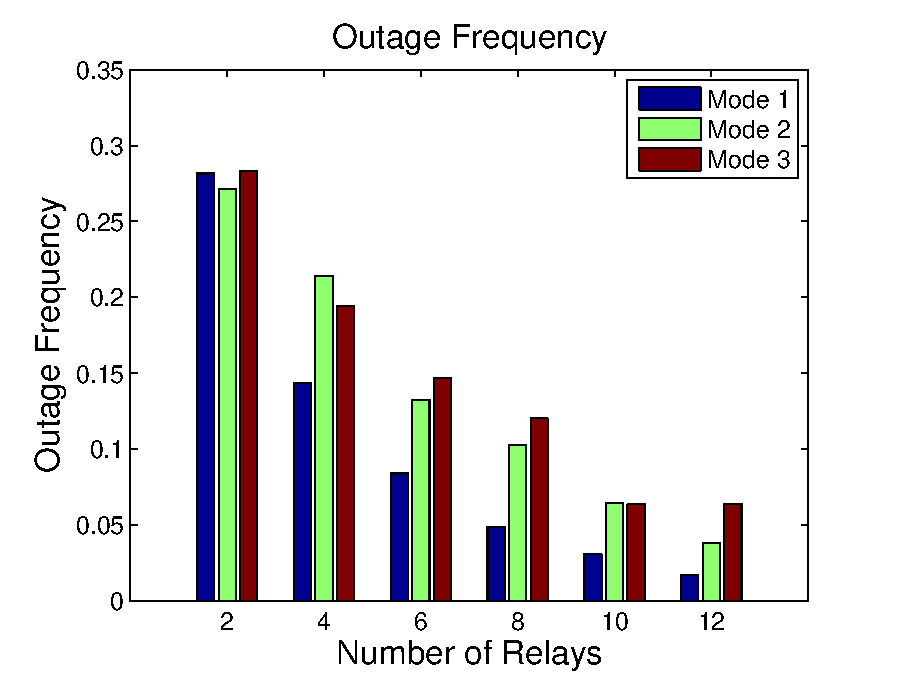
\includegraphics[width=12cm]{outagefrequency_V2.eps}
\caption{Outage Frequency of Three Modes with Different Relay Densities}
\label{outagefrequency}
\end{figure}
Figure \ref{outagefrequency} shows the result of outage frequency of the three different modes and different relay densities. From this result, we can see that Mode 1 performs better than Mode 2 and Mode 3. This is due to the randomness of the relay deployment, which works against outage prevention for this model. In some cases Mode 3 performs better than Mode 2. This occurs when most of the relays in Mode 2 are placed in deep shadow areas and are therefore ineffective.. The ideal relay deployment scheme would place relays at the edge of a deep fading area so that relays can successfully receive signals from the BS. On the average, random placement (Mode 3) is the worst choice among the three cases in our simulation.
\par For real-time applications, outage duration and outage frequency are both very important factors from the user experience point of view. Long outage duration and high outage frequency will lead to poor delay performance or even loss of packets. Figure \ref{outagefrequency} indicates that higher relay density will result in lower outage frequency. Next we investigate the outage duration experienced by the MS with different relay deployments. Outage duration performance is given in Figure \ref{Mode1Out}, \ref{Mode2Out} and \ref{Mode3Out}, which shows the cumulative distribution functions for outage durations for all three different modes. Here, we just show the distribution of outage duration from $100ms$ to $2s$ ($100ms$ is the smallest simulation time period). Under the SNR requirement given as $8dB$, it is shown that as the relay density increases, the probability of long outage duration decreases quickly. In Mode 1, with 4 relays, the probability of outage duration longer than $400ms$ is less than $10\%$. In Mode 2 and Mode 3, to achieve this, 6 and 8 relays are needed, respectively. For real-time video conferencing, the largest tolerable delay is around $200ms$. Our results indicate that in Mode 1 we do not need more than 6 relays to guarantee the probability of outage duration larger than $200ms$ to be less than $15\%$. In Mode 2 and Mode 3 more than 12 relays are needed to achieve this objective. Since we put the SNR requirement as $8dB$, which guarantees a small bit error rate (BER) of 16-QAM, the relay density needs to be high. If we reduce the SNR requirement and change the modulation, it is possible that the probability of outage duration longer than $200ms$ will become smaller or even close to 0. If there is no relay in the cell and an MS enters into a deep fading area, then due to correlated shadow fading, this outage duration will last for a long time. The longest outage duration in our simulation is $10s$ with no relay. From Figure \ref{Mode1Out}, \ref{Mode2Out} and \ref{Mode3Out} we can observe that the probability of an outage duration greater than $2s$ is approximately $5\%$ without relaying. Comparing the no relay case with the 6 relays case in Mode 1, it is shown that relays efficiently reduce the lengthy outages which are caused by deep shadow fading, with the probability of outage duration greater than $2s$ reduced to less than $1\%$. All these results indicate that relays can mitigate the deleterious effects of correlated shadow fading efficiently.

\section{Conclusions and Future Work}
\label{sec:Conclusions}
In this chapter, we investigate the correlated shadow fading problem in a single cell cellular network and shows that it could lead to correlated outage and long outage durations. A correlated outage field is presented in this chapter. To mitigate shadow fading, relays can be deployed. The performance of three different relay deployments with different relay densities are studied. Theoretical analysis and simulations of outage performance are given to compare between different relay placement scenarios. Through these simulation, we showed that uniformly spaced relays perform better than the randomly spaced, due to the randomness of relay deployment. In next several chapters, we will consider different shadow fading correlation model, which is more realistic to analyze multi-cell system. We will extend our analytic work to build a model that can predict the impact of shadow fading in a mobile environment to different parameter settings.







\chapter{System Performance Analysis under Exponential Correlated Shadow Fading}\label{ch:ExpSingleCell}
\par Shadow fading has been proven to be a significant contributor to channel variations in wireless communication. In most cases shadow fading is assumed to have a log-normal fading distribution to model the loss at a certain location. However, in a mobile network, it is also important to know how shadow fading is correlated both in space and in time, which can greatly affect application layer behavior and service quality. This chapter is an attempt to characterize shadow fading so as to accurately study its impact on the application layer quality of service. If the correlation is strong over time and space, shadow fading can result in a long outage. In this chapter, we assume shadow fading is exponentially correlated in space. To study correlated shadow fading and its resultant outage durations, a first-order Markov chain model is developed and validated. The Markov chain model is constructed by partitioning the entire shadow fading range into a finite number of intervals. The state transition matrix of the Markov chain is derived from the joint probability distribution of correlated log-normal shadow fading. Based on the proposed Markov chain model, the frequency and duration of outage near the edge of a single cell is analyzed. To validate the Markov chain model, correlated Gaussian random fields are simulated to analyze the outage frequency and durations due to correlated shadow fading. Comparing the simulation results with the Markov chain model results, we can conclude that the proposed Markov chain model is an efficient way to describe the channel variations, and the user experienced outage behavior of the channel.
\section{Background}
In the past few decades, fading in wireless communication systems has been studied extensively in the literature. Fading phenomena can substantially affect the performance of a wireless communication system. In general, fading can be divided into two categories: large-scale fading and small-scale fading. A signal transmitted from source to destination will experience both large-scale and small-scale fading. Small-scale fading is caused by multipath propagation. Large-scale fading, which is also known as shadow fading, is caused by obstacles (trees, buildings, etc.) in the propagation path. Shadow fading is approximated by an independent log-normal distribution \cite{rappaport1996wireless} in most cases. Researchers have also shown that shadow fading is spatially correlated at different positions on the propagation path \cite{gudmundson1991correlation}, \cite{zhang2008novel}. The spatial correlation of shadow fading is important when studying the quality of service of a mobile system since it will result in long-lasting outage durations, which will deteriorate the performance of the applications running on the network. For example, in Figure \ref{building}, the user is moving behind a row of tall buildings which block the signals from the base station. These tall buildings result in deep shadow fading, and the shadow fading of different positions behind these buildings are closely correlated.
\begin{figure}
\centering
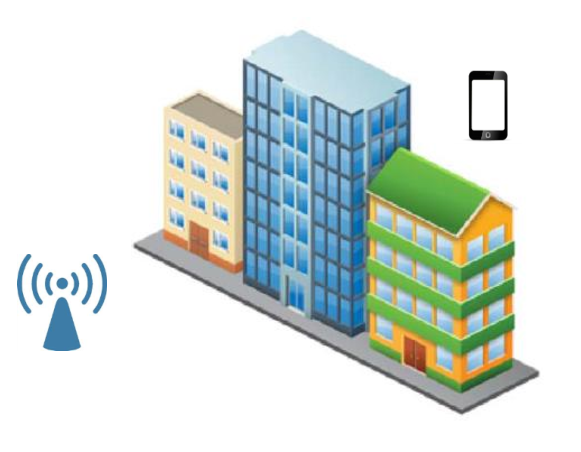
\includegraphics[width=6cm]{building.eps}
\caption{An example of building blockage.}
\label{building}
\end{figure}
\par The spatial correlation of shadow fading has been investigated by numerous researchers. Based on empirical measurements, different autocorrelation models have been proposed for different scenarios and radio frequencies \cite{gudmundson1991correlation, sorensen1998correlation, weitzen2002measurement}. Szyszkowicz et al. \cite{szyszkowicz2010feasibility} studied shadow fading correlation models and investigated the feasibility of all these models. Among all these models, the analytical model proposed by Gudmundson \cite{gudmundson1991correlation} based on empirical measurements of $900MHz$ frequency is the one which is widely used in channel estimation. This model shows that shadow fading can be modeled as a first-order autoregressive process AR(1), which indicates a spatial exponential decaying autocorrelation function. Given this model, we propose a Markov chain model that can be constructed to capture the variation of shadow fading. The Markov chain models can in turn be used to accurately model the impact of shadow fading on higher layer protocols and applications. Since the shadow fading statistically follows a log-normal distribution, we can divide the entire range of shadow fading, which is $[-\infty,+\infty]$ into a finite number of intervals. Each interval is considered as a state of the Markov chain model. When the shadow fading falls in a particular interval, it is assigned to be in this particular state. The number of intervals (states) defines the granularity of the Markov chain model. The higher the number of states, the higher the precision in modeling the shadow fading. Correlated log-normal shadow fading has different variances with regard to different scenarios. For example, urban and suburban areas have different standard deviations based on empirical measurements. Different standard deviations of the log-normal shadow fading will result in different state transition matrices of the Markov chain model.
\par Outage events happen when the channel state is poor, and the received signals are not strong enough for the receiver to decode. Outage probability and the length of outage duration are important performance measurements of a wireless communication system over fading channels. Considering the applications which require low latency where buffer size is small, a long outage duration will drop the connection and lower the quality of service. To study the outage behavior of a communication system under correlated shadow fading, a well designed Markov chain model is a powerful tool. With a Markov chain model, the channel state in the next user position can be estimated from the current channel state given the current user position. Therefore, the system performance can be evaluated efficiently. Fading is a significant factor which causes dramatic channel state variations. Correlated shadow fading will result in long-lasting outage durations which is harmful to delay-sensitive real-time application and result in loss of quality of service. The Markov chain model can be used to analyze the probability distribution of outage events. The distribution and behavior of outage events will provide us the necessary information to improve wireless communication systems further. For example, efficient cooperative communication schemes can be designed to mitigate the outage behavior.
\par The main focus of this chapter is how to design a first-order Markov chain model to reflect the spatial correlation of shadow fading, and the study of outage behavior of a single cell wireless communication system given correlated shadow fading. The key contributions of this chapter are summarized below.
\begin{itemize}
\item Constructed a Markov chain model based on correlated shadow fading.
%\item Studied the proper number of states of the Markov chain model and validated it through simulation. \reminder{this is not a contribution since you just tried several options}
\item Analyzed the outage frequency and outage duration of a single cell wireless communication system over correlated shadow fading.
\end{itemize}
 The remaining sections of this chapter are organized as follows. The channel model with spatial correlated shadow fading is described in Section~\ref{sec:shadowing}. Section~\ref{sec:markov} shows how to construct the Markov chain model from the correlated shadow fading. Analysis of outage behavior is demonstrated in Section~\ref{sec:outage}. Simulation to validate the Markov chain model is illustrated in Section~\ref{sec:simulation}. Section~\ref{sec:conclusion} summarizes and concludes the chapter.
\section{Channel Model with Correlated Shadow Fading}
\label{sec:shadowing}
\begin{figure*}
\centering
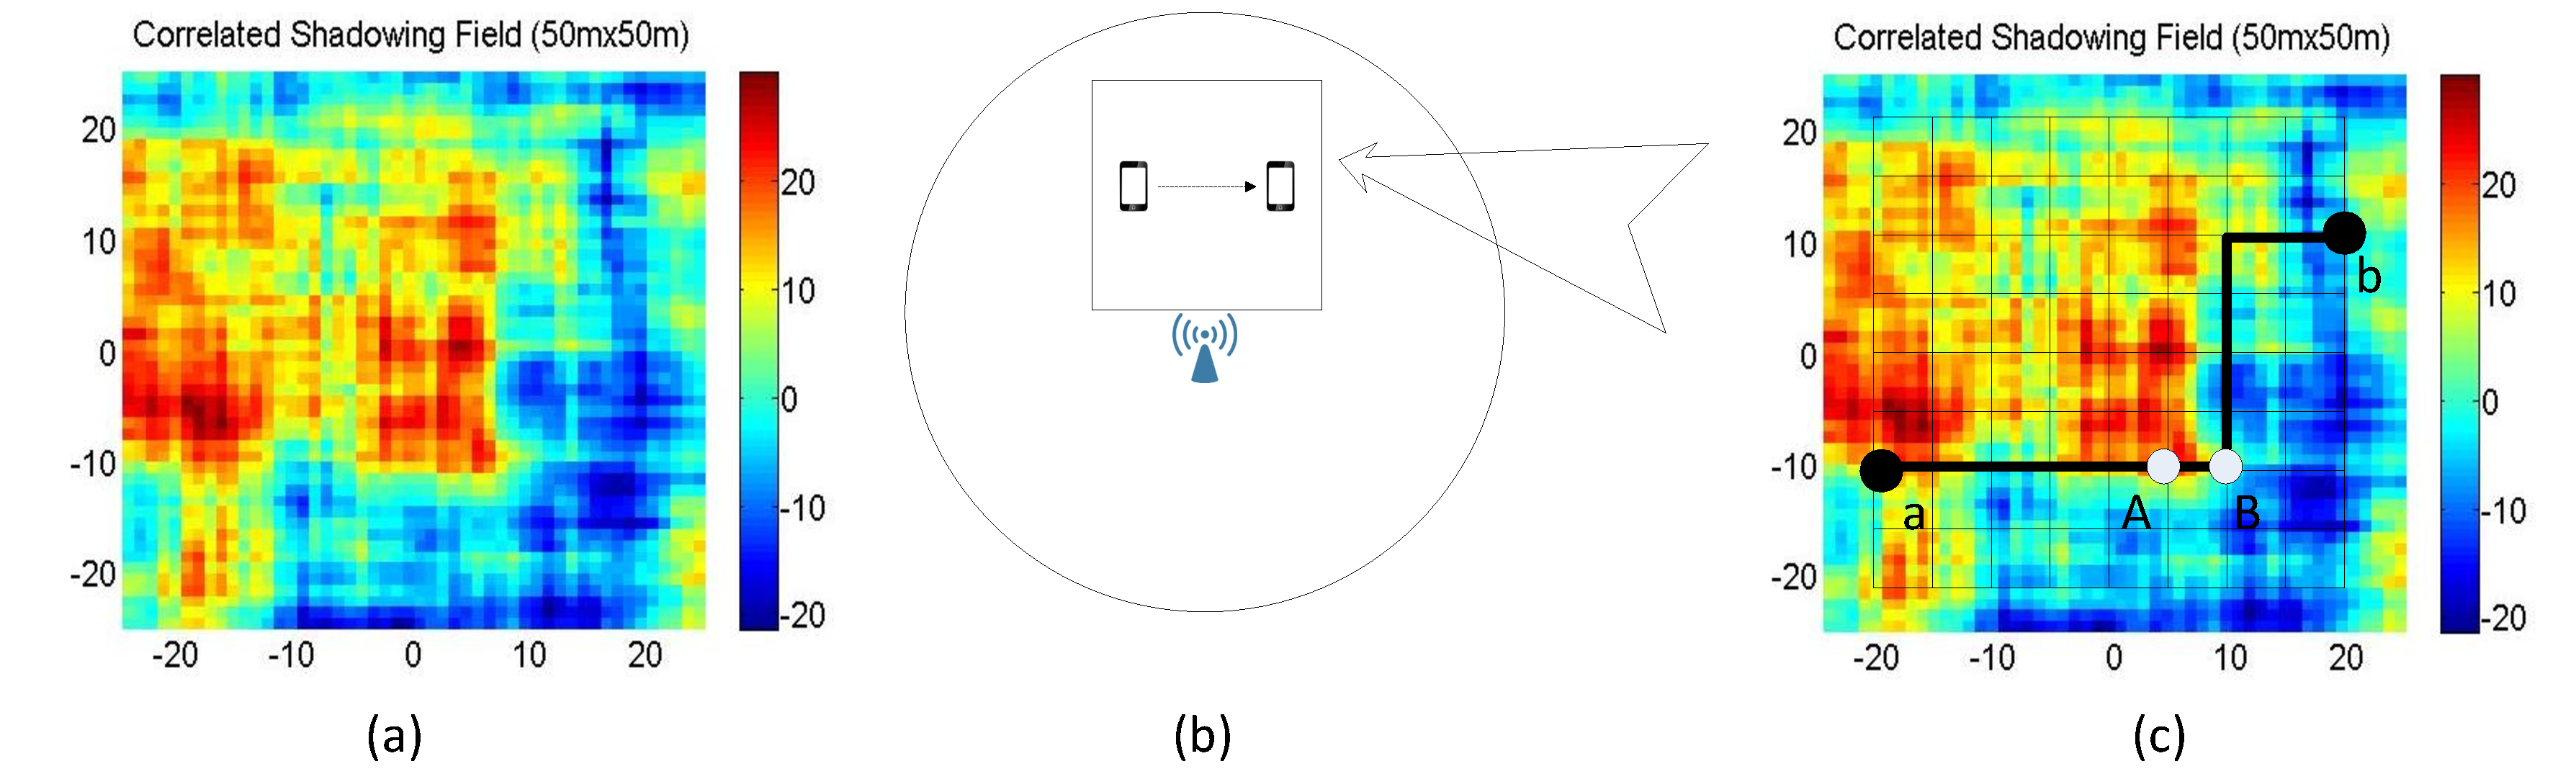
\includegraphics[width=14cm]{finalsystemab_V3.eps}
\caption{(a) A typical exponential correlated shadow fading field in a $50m\times50m$ area. The color bar denotes the value of the shadow fading in dB. (b) A single cell model with a MS moving on a fixed trajectory. (c) A locally generated correlated shadowing field for a fixed trajectory from point a to point b.}
\label{systemmodel}
\end{figure*}
To simplify the problem, we consider a single 4G LTE cell without any intercell interference in Figure \ref{systemmodel}(b). Due to the high bandwidth of OFDM systems,  LTE networks are more resilient to frequency selective fading \cite{rappaport1996wireless}, therefore in this paper small-scale fading is ignored and shadow fading becomes the most important fading factor. There is a Base Station(BS) at the center of the cell. A Mobile Station (MS) is moving on a certain trajectory within the cell. The received signal on a link $(S\to D)$ between source and destination is given by:
\begin{equation}
y_{D} = G_{SD}x_{S}+n_{D}.
\end{equation}
where $x_{S}$ is the signal transmitted by the source and $y_{D}$ is the signal received by the destination. $n_{D}\sim \mathcal{CN}(0,N_{0})$ is additive white Gaussian noise. $G_{SD}$ is the channel gain from source to destination including path loss and shadow fading.  $\text{SNR} \triangleq P*G_{SD}^{2}/N_{0}$, is the end-to-end received signal-to-noise ratio (SNR). The destination successfully receives the signals if no outage event happens, i.e., $\log_{2}(1+\text{SNR})\ge R$, where $R$ is the required data rate. From the definition of SNR, no outage event happens as long as $G_{SD}^2 > \beta$, where $\beta = \frac{(2^{R}-1)*N_{0}}{P}$. Therefore the channel gain from transmitter to receiver determines if an outage will occur.
\par Here we rewrite the channel gain in the following form: $G_{dB}=PL(d)+S$, where $G_{dB}$ is $G_{SD}$ in $dB$, $PL$ denotes the propagation pathloss in $dB$, $d$ is the distance from BS to MS and $S$ denotes shadow fading factor. In most cases, shadow fading is modeled as an independent log-normal distribution \cite{goldsmith2005wireless} with a standard deviation derived from empirical measurements. In this model, the probability distribution of pathloss $G_{dB}$ is given by:
\begin{equation}
p(G_{dB})=\frac{1}{\sqrt{2\pi}\sigma_{G_{dB}}}exp[-\frac{(G_{dB}-\mu_{G_{dB})^2}}{2\sigma_{G_{dB}}^2}].
\end{equation}
where $\mu_{G_{dB}}$ is the average pathloss which is equal to $PL(d)$ and $\sigma_{G_{dB}}$ denotes the standard deviation of pathloss. Since shadow fading is the only fading factor that is considered here, $\sigma_{G_{dB}}$ is determined by the standard deviation of shadow fading.
This model fails to capture the spatial correlations in shadow fading. For examples, in Figure \ref{systemmodel}(c), shadow fading factors of two close positions A and B, which are $S_{A}$ and $S_{B}$, are not independent but correlated to each other. Empirical measurements showed that shadowing has significant correlations in several realistic scenarios and the correlated shadow fading can affect system performance \cite{graziano1978propagation}. Among all models derived from empirical measurements for correlated shadow fading, exponentially decaying correlation \cite{gudmundson1991correlation} is widely used. In this paper, we choose this model to do further analysis. Figure \ref{systemmodel}(a) is an example of exponentially correlated shadowing field which is generated from the Graziano model \cite{graziano1978propagation}. This figure shows a $50\times50 m^{2}$ shadow fading area and illustrates that deep shadowing area is clustered and correlated (the blue area).
\par In Figure ~\ref{systemmodel}(c), the entire space is discretized. The MS moves on the lattice as shown. $A$ and $B$ are two neighbouring points. Assume the shadow fading (in dB) is $N(0,\sigma^{2})$ where $\sigma$ is the standard deviation, the spatial correlation between $S_{A}$ and $S_{B}$ will be given by
\begin{equation}
\rho_{A,B}=\frac{E[S_{A}S_{B}]}{\sigma^{2}}=e^{{-\frac{d_{A,B}}{d_{0}}}}
\end{equation}
where $d_{A,B}$ is the distance between $A$ and $B$, $d_{0}$ denotes the de-correlation distance \cite{bertoni1999radio}, which means if the distance between two points are substantially greater than $d_{0}$, the two shadow fading will be independent to each other. $d_{0}$ is determined by the environment, therefore urban and suburban areas have different de-correlation distances. An exponential correlation implies the shadow fading samples can be written as an AR(1) process as follows \cite{wei1994time}:
\begin{equation}
S_{B} = \rho S_{A} + (1-\rho)n_{A}
\label{e3}
\end{equation}
where $n_{A}$ denotes the channel noise at $A$. From this we conclude that the next channel state can be determined from the current channel state and the distance MS moves.
\section{Markov Chain Model}
\label{sec:markov}
In this section, we will construct a Markov chain model for exponential correlated shadow fading. First of all, we will discretize the space. In Figure \ref{systemmodel}(c), the space was partitioned into unit square spaces of $5\times5m^{2}$ (This granularity is used to describe the Markov chain model while in the simulation we uses a finer granularity). The MS moves on the lattices from point to point, the distance between each two neighboring points are considered as a unit distance $\delta d$. We prove that shadow fading factors of any two points that can be connected by a trajectory having jointly Gaussian distribution.
\begin{lem}
\emph{Exponential correlated shadow fading factors of any two points that can be connected by a trajectory have a jointly Gaussian distribution.}
\end{lem}
\begin{proof}Suppose the two points are $a$ and $b$, since there exists a trajectory connecting $a$ and $b$ like in Figure \ref{systemmodel}(c), we can assume there are $n$ positions on this trajectory $(t_{1},t_{2},\dots,t_{n})$. Then follow equation (\ref{e3}), we have the following:
\begin{equation}
\label{e5}
\begin{split}
S_{b} &=\rho S_{t_{n}}+(1-\rho)n_{t_{n}}\\
&=\rho(\rho S_{t_{n-1}}+(1-\rho)n_{t_{n-1}})+(1-\rho)n_{t_{n}}\\
&=\ldots\ldots\\
&=\rho^{n}S_{t_{1}}+\sum_{i=1}^{n}\rho^{n-i}(1-\rho)n_{t_{i}}\\
&=\rho^{n+1}S_{a}+\rho(1-\rho)n_{a}+\sum_{i=1}^{n}\rho^{n-i}(1-\rho)n_{t_{i}}
\end{split}
\end{equation}
Let $X=\alpha S_{a}+\beta S_{b}$, from equation ~\ref{e5}, the following can be derived:
\begin{equation}
X=\alpha S_{a}+\beta(\rho^{n+1}S_{a}+\rho(1-\rho)n_{a}+\sum_{i=1}^{n}\rho^{n-i}(1-\rho)n_{t_{i}})
\end{equation}
Since $S_{a}$, $n_{t_{i}}$ and $n_{a}$ are all independent and Gaussian random variables, we conclude that $X$ is also Gaussian, which implies that $S_{a}$ and $S_{b}$ are jointly Gaussian.
\end{proof}
\par Given the above conclusion, a Markov chain model can be constructed as follows:
\begin{itemize}
\item Divide the entire shadow fading range $[-\infty,+\infty]$ into a finite number of intervals $\{[-\infty,S_{0}],[S_{0},S_{1}],\dots,[S_{N},+\infty]\}$. Each interval represents a state of the Markov chain model.
\item Derive the state transition matrix of the Markov chain model from the probability distribution of the correlated shadow fading.
\item Derive the steady-state probability from the state transition matrix of the Markov chain model.
\end{itemize}
\par To derive the state transition matrix of the Markov chain model, we first investigate the probability density function of the correlated shadow fading. Since we have discretized the entire space into unit distances, here the state transition probability from point $A$ to point $B$ will be defined and used to calculate the state transition matrix of the Markov chain. Since $S_{A}$ and $S_{B}$ are jointly Gaussian with a correlated coefficient $\rho_{0}$, according to \cite{papoulis2002probability}, we have
\begin{equation}
\begin{split}
& f_{S_{A}|S_{B} =s_{B}}(s_{A}) =\frac{f_{S_{A},S_{B}}(s_{A},s_{B})}{f_{S_{B}}(s_{B})}\\
&=\frac{1}{\sigma_{A}\sqrt{2\pi(1-\rho_{0}^{2})}}\exp\{-\frac{(s_{A}-(\mu_{A}+\sigma_{A}\rho_{0}(s_{B}-\mu_{B})/\sigma_{B}))}{2\sigma_{A}^{2}(1-\rho_{0}^{2})}\}
\end{split}
\end{equation}
where $\mu_{A}$ and $\mu_{B}$ are expectations of log-normal shadow fading $S_{A}$ and $S_{B}$, which is typically set to $0$, while $\sigma_{A}$ and $\sigma_{B}$ are standard deviations, which are assumed to be equal to $\sigma_{0}$. Based on these assumptions, we can rewrite the equation as follows:
\begin{equation}
f_{S_{A}|S_{B} =s_{B}}(s_{A}) =\frac{1}{\sigma_{0}\sqrt{2\pi(1-\rho_{0}^{2})}}\exp\{-\frac{s_{A}-\rho_{0}s_{B}}{2\sigma_{0}^{2}(1-\rho_{0}^{2})}\}
\end{equation}
Assume there are $N$ states of the Markov chain model $ST_{1}, ST_{2},\cdots, ST_{N}$ where $ST_{i}$ corresponds to the interval $(S_{i-1}, S_{i}]$. Then we have the state transition probability as follows:
\begin{equation}
\label{statetransition}
\begin{split}
P_{i,j} &= P(S_{A}\in ST_{j}|S_{B}\in ST_{i})\\
&=\frac{P(S_{A}\in ST_{j}, S_{B}\in ST_{i})}{P(S_{B}\in ST_{i})}\\
&=\frac{\int_{S_{i-1}}^{S_{i}}(\int_{S_{j-1}}^{S_{j}}f_{(S_{A}|S_{B}=s_{B}}(s_{A})ds_{A})f(s_{B})ds_{B}}{\int_{S_{i-1}}^{S_{i}}f(s_{B})ds_{B}}
\end{split}
\end{equation}
From equation (\ref{statetransition}), the state transition matrix of the Markov chain can be derived. The steady-state transition matrix can be determined by $P$.
\section{Analysis of Outage Behavior}
\label{sec:outage}
In this section we analyze the outage behavior of the communication system using the Markov chain model of correlated shadow fading. The outage duration of a system is a significant factor influencing system performance. Given a fixed mobile trajectory, the Markov chain model described in Section \ref{sec:markov} provides an efficient way to study the outage events. In Figure \ref{systemmodel}(c), a fixed trajectory is given from point $a$ to $b$ through several intermediate points. Considering two consecutive points $A$ and $B$, we have $G_{A}=PL_{A}(d_{A})+S_{A}$ and $G_{B}=PL_{B}(d_{B})+S_{B}$ in $dB$. The probability that $A$ and $B$ are both in an outage area can be written as:
\begin{equation}
\begin{split}
&P(G_{A}<\gamma, G_{B}<\gamma) \\
&= P(S_{A}<\gamma-PL_{A}(d_{A}), S_{B}<\gamma-PL_{B}(d_{B}))
\end{split}
\end{equation}
%\begin{figure}
%\centering
%\includegraphics
%\caption
%\label{trajectory}
%\end{figure}
If $S_{A}<\gamma-PL_{A}(d_{A}) \in ST_{i}$ and $S_{B}<\gamma-PL_{B}(d_{B}) \in ST_{j}$, we can infer that, to avoid outage, the lower bound of the shadow fading factor $S_{A}$ is in state $ST_{i}$ and for $S_{B}$ is in state $ST_{j}$. State $ST_{i}$ and $ST_{j}$ are called lower bound states. Based on this approximation, the above probability can be written as:
\begin{equation}
P(G_{A}<\gamma, G_{B}<\gamma)=\sum_{m=0}^{i}\sum_{n=0}^{j} P(ST_{m})\bullet P(ST_{m},ST_{n})
\end{equation}
where $P(ST_{m})$ is the probability that $S_{A}$ is in the range of $ST_{m}$ which can be calculated from the Gaussian distribution. $P(ST_{m},ST_{n})$ can be found from the state transition matrix. Following this, the probability of an outage duration of length $l>L$ can be derived in below:
\begin{equation}
\begin{split}
&P(G_{1}<\gamma,\dots,G_{L}<\gamma)=\\
&\sum_{m_{1}=0}^{M_{1}}\dots\sum_{m_{L}=0}^{M_{L}} P(ST_{m_{1}})\bullet P(ST_{m_{1}},ST_{m_{2}})\\
&\bullet\dots\bullet P(ST_{m_{L-1}},ST_{m_{L}})
\end{split}
\end{equation}
where $M_{i}$, $i\in\{1,\dots,L\}$ are corresponding lower bound states of each position on the trajectory.
\section{Simulation Results}
\label{sec:simulation}
\begin{table*}
\begin{equation}
P=\begin{bmatrix}
\begin{smallmatrix}
0.5580 & 0.3627 & 0.0757 & 0.0036 & 3.5243\times10^{-5} & 0 & 0 & 0 \\
0.1587 & 0.4404 & 0.3359 & 0.0624 & 0.0026 & 2.3466\times10^{-5} & 0 & 0 \\
0.0184 & 0.1788 & 0.4546 & 0.2980 & 0.0484 & 0.0018 & 1.4485\times10^{-5} & 0 \\
0.0007 & 0.0258 & 0.2165 & 0.4624 & 0.2573 & 0.0361 & 0.0012 & 8.4341\times10^{-6} \\
8.4341\times10^{-6} & 0.0012 & 0.0361 & 0.2573 & 0.4624 & 0.2165 & 0.0258 & 0.0007 \\
0 & 1.4485\times10^{-5} & 0.0018 & 0.0484 & 0.2980 & 0.4546 & 0.1788 & 0.0184 \\
0 & 0 & 2.3466\times10^{-5} & 0.0026 & 0.0623 & 0.3359 & 0.4404 & 0.1587 \\
0 & 0 & 0 & 3.5243\times10^{-5} & 0.0036 & 0.0757 & 0.3627 & 0.5580 \\
\end{smallmatrix}
\end{bmatrix}
\label{matrix}
\end{equation}
\end{table*}
\par In this section, we employ Monte-Carlo simulation to validate our Markov chain model. To start the simulation, a large number of correlated shadowing fields are generated. As shown in Figure \ref{systemmodel}(b) and (c), instead of generating shadowing fields for the entire cell, we pick up a MS trajectory and generated shadowing fields that covers that trajectory. In this paper, we choose the urban environment as the case to study. In this case, the shadow fading and Markov chain parameters are set as in Table \ref{SystemConfig}. The standard deviation of shadow fading is chosen to be $8dB$ following \cite{szyszkowicz2010feasibility}. The number of states of the Markov chain is set to be $3*\sigma_{0}/n*2+2$, where $n=1,3,8$ is the size of each range (state) in $dB$ except the two above $3\sigma_{0}$. $n$ in this case represents different granularities in the area of $[-3\sigma_{0},3\sigma_{0}]$. The state transition matrices are calculated with regard to each $n$. For example, when $n=8$, the states of the Markov chain model are:
\begin{equation}
\begin{split}
[&(-\infty,-24],(-24,-16],(-16,-8],(-8,0],\\
&[0,8],[8,16),[16,24),[24,+\infty)]
\end{split}
\end{equation} and the state transition matrix is given in (\ref{matrix}).
\begin{table}
\centering
\caption{\label{SystemConfig}Simulation Configuration Parameters}

\begin{tabular}{|c|c|}

\hline

\multirow{2}{*}{Okumura-Hata Model} & BS Height: $100m$\\
& MS Height: $1m$\\
\hline
%Rayleigh Fading & Coherence Time: $100ms$\\
%\hline
\multirow{5}{*}{Correlated Shadow Fading}
& De-Correlation Distance $d_{0}$: $20m$\\
& Standard Deviation $\sigma_{0}$: $8dB$\\
\hline
\multirow{3}{*}{Markov Chain Model} & Number of States:\\
& 50, 18, 8\\
& ($3*\sigma_{0}/n*2+2$, $n=1, 3, 8$)\\
\hline
MS Trajectory & Unit Distance $\delta d$: $1m$\\
\hline
Shadowing Field & $50\times50m^{2}$\\
\hline
Radio Frequency & $f: 1024MHz$\\
\hline
BS Transmission Power & $P: 30dbm$\\
\hline
SNR Requirement & $10dB$\\
\hline
\end{tabular}
\end{table}
\par To validate our Markov chain models, the probability distributions of outage durations corresponding to MS trajectories of length $l>1m$ up to $l>9m$ are studied given different number of states. Since there is a trade-off between the number of states and the complexity of the simulation computation, the simulated results also provide us information about the proper granularity of the Markov chain model to most accurately approximate the real channel. The simulation also confirms that correlated shadow fading indeed can cause long-lasting outage durations. In our simulation, the MS moves on a straight track which is around $900m$ away from the BS. Let $l$ denote the outage duration in meters, Figure \ref{prob} shows the probability of $l>L$. Comparing the two cases: with and without correlation, we can conclude that correlated shadow fading can result in severe long-lasting outage durations. Take $L=5$ for example, the correlated case gives $P(l>L)=12\%$, while in the non-correlated case the probability is around $0\%$. This illustrates the correlation between shadow fading cannot be neglected in mobility models. The MS speed is approximately the same as pedestrian speed which is $1m/s$ (Since the edge length of the lattice is $1m$, the MS moves one grid (unit distance) every second). Assuming this, the user will experience an outage of more than $9$ seconds with a probability of $7\%$.
\par To find out the proper number of states of the Markov chain model, three different Markov chain models with different number of states are tested. Basically we divide the $[-3\sigma_{0},3\sigma_{0}]$ area with different granularity, which is represented by $n=1,3,8$. When $n=1$, the interval $ST_{i}$ except $(-\infty,S_{0}]$ and $[S_{N},+\infty)$ is $1dB$. The results showed in Figure \ref{prob} indicates that when $n=1$, the curve is close to the correlation curve, which means that the Markov chain model becomes a good approximation of the channel to study the outage behavior of the system. Generally, more Markov states lead to more precise models. When the interval $[S_{i},S_{j}]$ becomes relatively large with regarding $\sigma_{0}$, the Markov chain model will fail to be a useful tool to study the outage behavior of the system. For example, in Figure \ref{prob}, when $n=8$, $P(l>1)$ is almost twice the correct $P(l>1)$. The prediction of the outage behavior of the system is not precise and useful anymore.
\begin{figure}
\centering
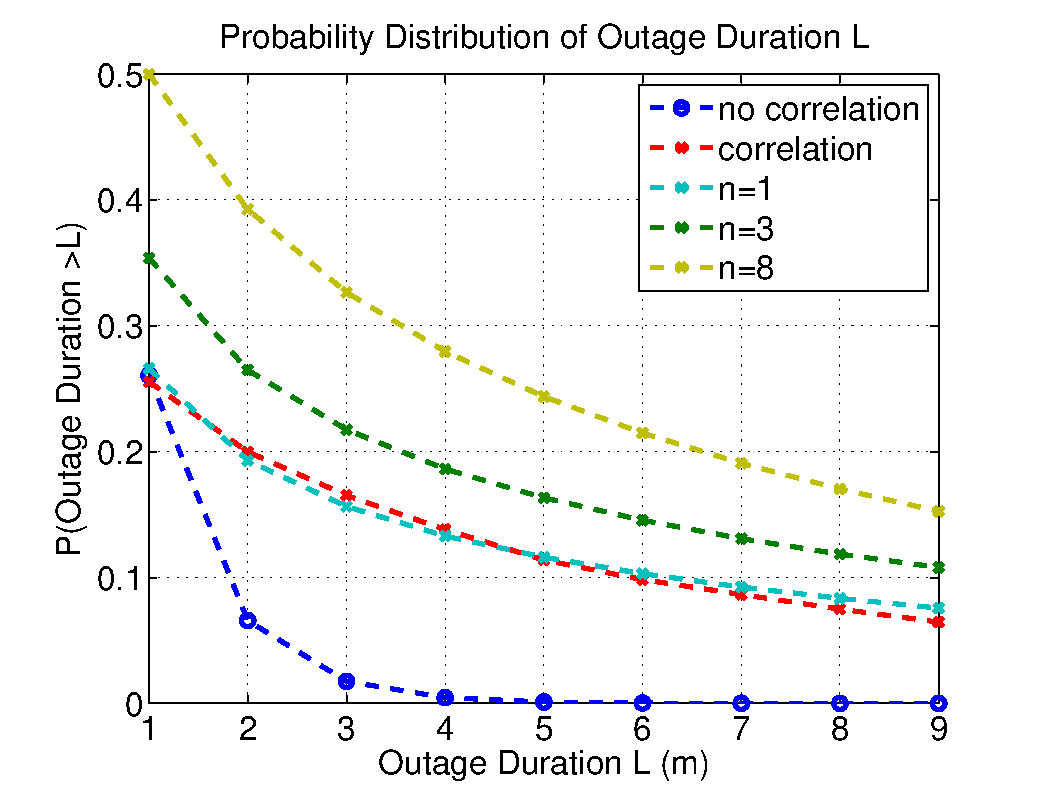
\includegraphics[width=9cm]{result_Plot_new.eps}
\caption{Probabilities of outage duration greater than $L$.}
\label{prob}
\end{figure}

\section{Conclusions}
\label{sec:conclusion}
\par In this chapter we investigated how shadow fading at different positions in a cellular network is correlated. In an environment where the correlation is high, shadow fading will result in long-lasting outage durations which can lead to a significant deterioration in system performance. To model spatially correlated shadow fading we divided the entire range of shadow fading into a finite number of intervals. A Markov chain model is then constructed, where each interval becomes a state of the Markov chain model. This model can be used to analyze the  outage behavior at the application layer. We demonstrated that a well designed Markov chain model with an appropriate number of states corresponding to the standard deviation of the shadow fading is indeed a powerful tool to study system performance. 
%In future work, we will use this model to study the impact of shadow fading at the transport and higher layers.

\chapter{Multi-Cell System Performance under Exponential Correlated Shadow Fading}\label{ch:4}
 \par In a multi-cell cellular network, connections between the Base Station (BS) and Mobile Users (MUs) may fail when the channel has low signal-to-interference-plus-noise ratio (SINR). Shadow fading is large-scale fading which can cause significant received power loss and reduce SINR for a wide area. Correlated shadow fading will result in correlated long-lasting outage durations in a multi-cell system. Increasing the BS density to make the network becomes denser is considered to be a way to increase SINR, reduce long-lasting outage durations and provide better Quality of Service (QoS) support for delay sensitive applications in noise-limited regime. In Chapter \ref{ch:2} and Chapter \ref{ch:3}, we discuss mitigating shadow fading in a single-cell model. This chapter extends the work in Chapter \ref{ch:3} and focuses on the study of the performance of a multi-cell communication system under correlated shadow fading. We consider the downlink direction in a multi-cell communication system. Two system layouts, Grid model and Random model, are studied to investigate the outage probability given correlated shadow fading and different BS densities. First, we compare the outage probability of two different BS layout models with same correlated shadow fading. Simulation results indicate that the Grid model performs better than the Random model. Secondly, the outage probability with independent shadow fading and correlated shadow fading for the Random model are demonstrated. SINR is calculated by assuming independent shadow fading and correlated shadow fading. Thirdly, we focus on Random model which is more realistic and present the distribution of outage durations while experiencing independent shadow fading or correlated shadow fading. Simulation results demonstrate that outage durations with correlated shadow fading are longer than those with the independent shadow fading. At last, we show that increasing the BS density can mitigate the effect of correlated shadow fading and improve the system performance by reducing outage probability and shortening outage durations. 
 \section{Background}
 %\par In a cellular communication system, the connection between the BS and a MU may be dropped when the user enters a deeply shadowed area. Fading phenomena can substantially affect the performance of a wireless communication system. In general, fading can be divided into two categories: large-scale fading and small-scale fading. A signal transmitted from source to destination will experience both large-scale and small-scale fading. Small-scale fading is caused by multipath propagation. Large-scale fading, which is also known as shadow fading, is caused by obstacles (trees, buildings, etc.) in the propagation path. In most cases, shadow fading is assumed to be temporally and spatially independent \cite{rappaport1996wireless}.  Researchers have also shown that shadow fading is spatially correlated at different positions on the propagation path \cite{gudmundson1991correlation}, \cite{zhang2008novel}. In \cite{fabbri2009impact} and \cite{patwari2008effects}, the effects of correlated shadowing in connectivity is demonstrated, which indicates that reliable connectivity will be much more difficult to maintain than indicated by independent shadow fading models. The spatial correlation of shadow fading is important when studying the quality of service of a mobile system since it will result in long-lasting outage durations, which will deteriorate the performance of the applications running on the network. The focus of this chapter is to study channel variations and system performance due to correlated shadow fading in a multi-cell communication system and provide a solution to reduce the frequency and duration of dropped connections and improve system performance by increasing BS density.
 \par There have been a lot of studies on the outage probability of cellular communication systems \cite{abu1991outage, petrovic2013outage, emamian2014outage}. The author of \cite{vural2015effect} analyzed the outage probability and coverage area under independent and identically distributed (\emph{i.i.d}) shadow fading which includes Log-normal distribution, Weibull distribution and Gamma distribution. In contrast, there is much less work on the outage probability and outage duration given correlated shadow fading. The system performance of a multi-cell system given correlated shadow fading remains to be an open problem. In \cite{lu2015long} and \cite{lu2015shining} we studied the outage probability and outage duration distribution of a single-cell communication system under exponentially correlated shadow fading and distance-angle correlated shadow fading. For a single-cell model, exponentially correlated shadow fading can be modeled as a Markov Chain Model. Highly correlated shadow fading will result in long-lasting outage durations. In \cite{lu2015shining}, a single-cell model under distance-angle correlated shadow fading is investigated. The correlated shadow fading leads to correlated outage events and long-lasting outage durations. To overcome this, we proposed a cooperative communication scheme to mitigate shadow fading by deploying relay at the cell edge. Chapter \ref{ch:2} and Chapter \ref{ch:3} are limited to a single-cell model. In this chapter, we are going to extend the study to correlated shadow fading impact on a multi-cell model, and provide a solution to overcome the long-lasting outage durations.
 \par For multi-cell system, a new general model for the user SINR is developed using stochastic geometry \cite{andrews2011tractable}. The cellular network is modeled by placing BSs at locations as a homogeneous Poisson Point Process (PPP). The author concluded that under general fading, increasing the number of BS does not affect the coverage probability (so is the outage probability) as long as the MU is connecting to the nearest BS. Moreover, the paper did comparison between grid model and the random PPP model, concluded that a regular grid model provided the upper bound of the coverage probability while the PPP model provided the lower bound. The author also considered the effect of independent log-normal interference and concluded that the increasing log-normal interference increased the coverage probability which is counter-intuitive. However, in this paper the author did not consider the scenarios with correlated log-normal shadow fading. Nevertheless, only the coverage probability is studied, outage duration has not yet been analyzed. 
 \par A comparative study of random and grid topology of small cell network deployment was given in \cite{chen2012small}. In this paper, spatial outage probability and spatial average throughput versus the number of access points of the two different network deployments are illustrated under independent shadow fading. Approximate outage probability and capacity for $\kappa-\mu$ shadow fading is studied in \cite{kumar2015approximate}. $\kappa-\mu$ shadow fading includes one-side Gaussian, the Rayleigh, the Nakagami-m and the Rician. As we mentioned before, the empirical measurements didn't exhibit such complicated features of shadow fading. Therefore when investigating system performance under correlated shadow fading, those complex features are not of main focus.
 \par The key contributions of this chapter are summarized as below:
 \begin{itemize}
 \item Correlated outage fields are given to analyze the relationship between correlated shadow fading and correlated outage events. 
 \item Investigate outage probability of both Grid model and Random model given correlated shadow fading.
 \item Show how increasing the BS density helps mitigate correlated shadow fading for Random model in terms of reducing outage probability (coverage probability) and outage durations.
 \item Analyze the relation between the tunable parameter (de-correlation distance) of the correlated shadow fading model and the outage probabilities.
 \item Compare the system performance of different MU-BS connection strategies: MU connecting to the nearest BS and MU connecting to the BS providing strongest signal.
 \end{itemize}
 The chapter is organized as follows: Section \ref{4:CorrShadowField} presents the correlated shadow fading model that is used in this chapter and the resultant correlated outage field. Section \ref{4:SystemModel} illustrates the system model with two different BS deployments and investigates the outage probability given the two deployments. Section \ref{4:OutageProb} gives theoretical analysis of outage probability given correlated shadow fading. Section \ref{4:SimuProb} presents the simulation setup and analyzes the simulation results of different BS densities. Section \ref{4:Conclusion} summarizes the chapter and proposes future work directions.
 
 \section{Correlated Shadow Fading}
 \label{4:CorrShadowField}
 As stated in the Chapter \ref{ch:2}, empirical measurement shows that there exist different patterns of correlations between shadow fading at different positions. The independent log-normal shadow fading model, while very useful for static MS performance analysis, cannot reflect the spatial correlation of shadow fading between different locations. In this section, we will give a brief introduction of shadow fading models, including the model which will be utilized in this chapter.
 In Chapter \ref{ch:2}, a distance-angle correlation model is used and in Chapter \ref{ch:3} an exponential correlation model is used. The correlation matrix of distance-angle model is given below:
 \begin{equation}
 \mathbf{K}_{N\times N} = [ \sigma_{s}(\vec{r_{i}})\sigma_{s}(\vec{r_{j}})h(\vec{r_{i}}\vec{r_{j}})],
 \label{4:correlationmatrix}
 \end{equation}
 where $N$ paths interfere with path $\vec{r_{i}}$ and $\mathbf{E}\{S_{i}^{2}|\vec{r_{i}}\}=\sigma_{s}^{2}(\vec{r_{i}})$. This model assumes that in the correlation matrix, $h$ is separable with respect to the angle of arrival
 \begin{equation}
 \theta = |\angle\vec{r_{i}}-\angle\vec{r_{j}}|\in [0^{\circ},180^{\circ}],
 \end{equation}
 and the arrival distance ratio
 \begin{equation}
 R=|10\log_{10}r_{i}/r_{j}|=\frac{10}{\ln 10}|\ln r_{i}-\ln r_{j}|,
 \end{equation}
 \begin{equation}
 h(\vec{r_{i}},\vec{r_{j}})=max\{1-\theta/\theta_{0},0\}\cdot max\{1-R/R_{0},0\}.
 \label{4:eq:1}
 \end{equation}
 The correlation coefficients is a piece-wise linear function (\ref{4:eq:1}) of the angle of arrival and the arrival distance ratio. This correlation model is suitable for a single-cell model when there is only one BS at the center of the cell. However, considering a multi-cell model, there are quite a number of BSs at different places, both autocorrelation and cross-correlation need to be taken care of. It is not possible to choose a single BS as the center of the shadowing field. To incorporate both autocorrelation and cross-correlation, the simulation complexity will increase in dramatic order. Due to this feature, the distance-angle model is not chosen to analyze the performance of a mulit-cell system. In this chapter, we choose the exponential correlation model in Chapter \ref{ch:3}. An exponentially correlated shadowing field $S$ with shadow fading factor $s_{i}$ for each position $p_{i}$ has a correlation matrix as below:
 \begin{equation}
 \mathbf{K}_{N\times N} = [ \sigma_{s}(p_{i})\sigma_{s}(p_{j})\rho(i,j)],
 \label{correlationmatrix}
 \end{equation}
 where $N$ is the length of the shadowing field. Suppose $A$ and $B$ are two neighboring points, the shadow fading (in dB) is $N(0,\sigma^2)$ where $\sigma$ is the standard deviation. The spatial correlation between $s_{A}$ and $s_{B}$ will be given by 
 \begin{equation}
 \rho_{A,B} = \frac{E[s_{A}s_{B}]}{\sigma^2} =e^{-\frac{d_{A,B}}{d_{0}}}
 \end{equation}
 \begin{figure}
 \centering
 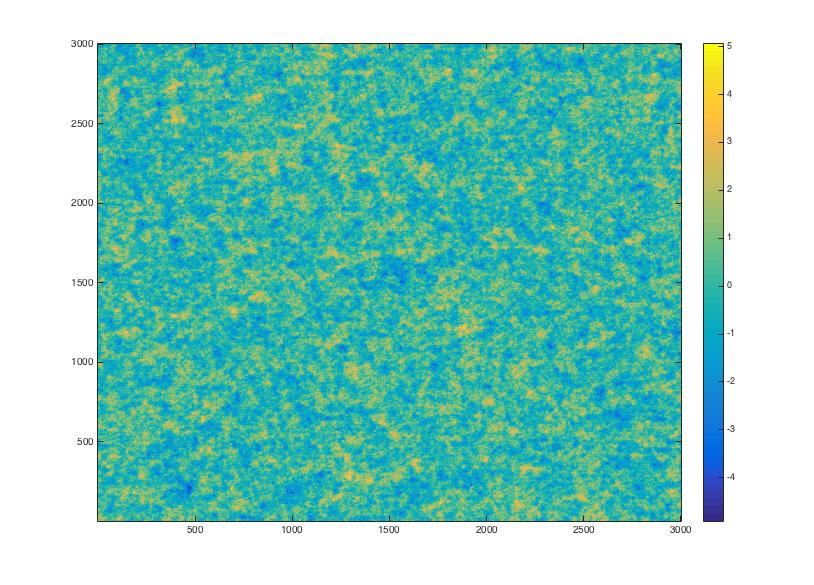
\includegraphics[width = 10cm]{ShadowFieldDeCorr20.jpg}
 \caption{Exponentially correlated shadowing field with $d_{0} = 20m$ (the color of the area refers to the normalized standard deviation which is $S_{i}/\sigma_{s}(i)$)}

 \label{ch4:shadowingfield}
 \end{figure}

 Following the shadowing field generation algorithm, we generate shadowing fields with different values of de-correlation distances. A sample shadowing field is shown in Figure \ref{ch4:shadowingfield} with $20m$ de-correlation distance.

 \par Given a correlated shadowing field, the outage events at different locations are correlated. Without considering other small-scale fading, the channel gain at different locations has a spatial correlation. An outage event occurs when SINR becomes less than $\gamma$, where $\gamma$ is a given SINR threshold. Based on the aforementioned correlated shadow fading model and Random system model, a correlated outage filed can be generated as in Figure \ref{4:outagefie}. On the left, an outage field with independent log-normal shadow fading is shown while the correlated outage field with correlated shadow fading is given on the right. The black color indicates outage areas. The outage area due to independent shadow fading are nonconsecutive dots. In contrast, it contains several connected areas under correlated shadow fading. Therefore, we conclude that correlated shadow fading results in correlated outage areas with regard to a multi-cell system.

 \begin{figure*}
 \centering
 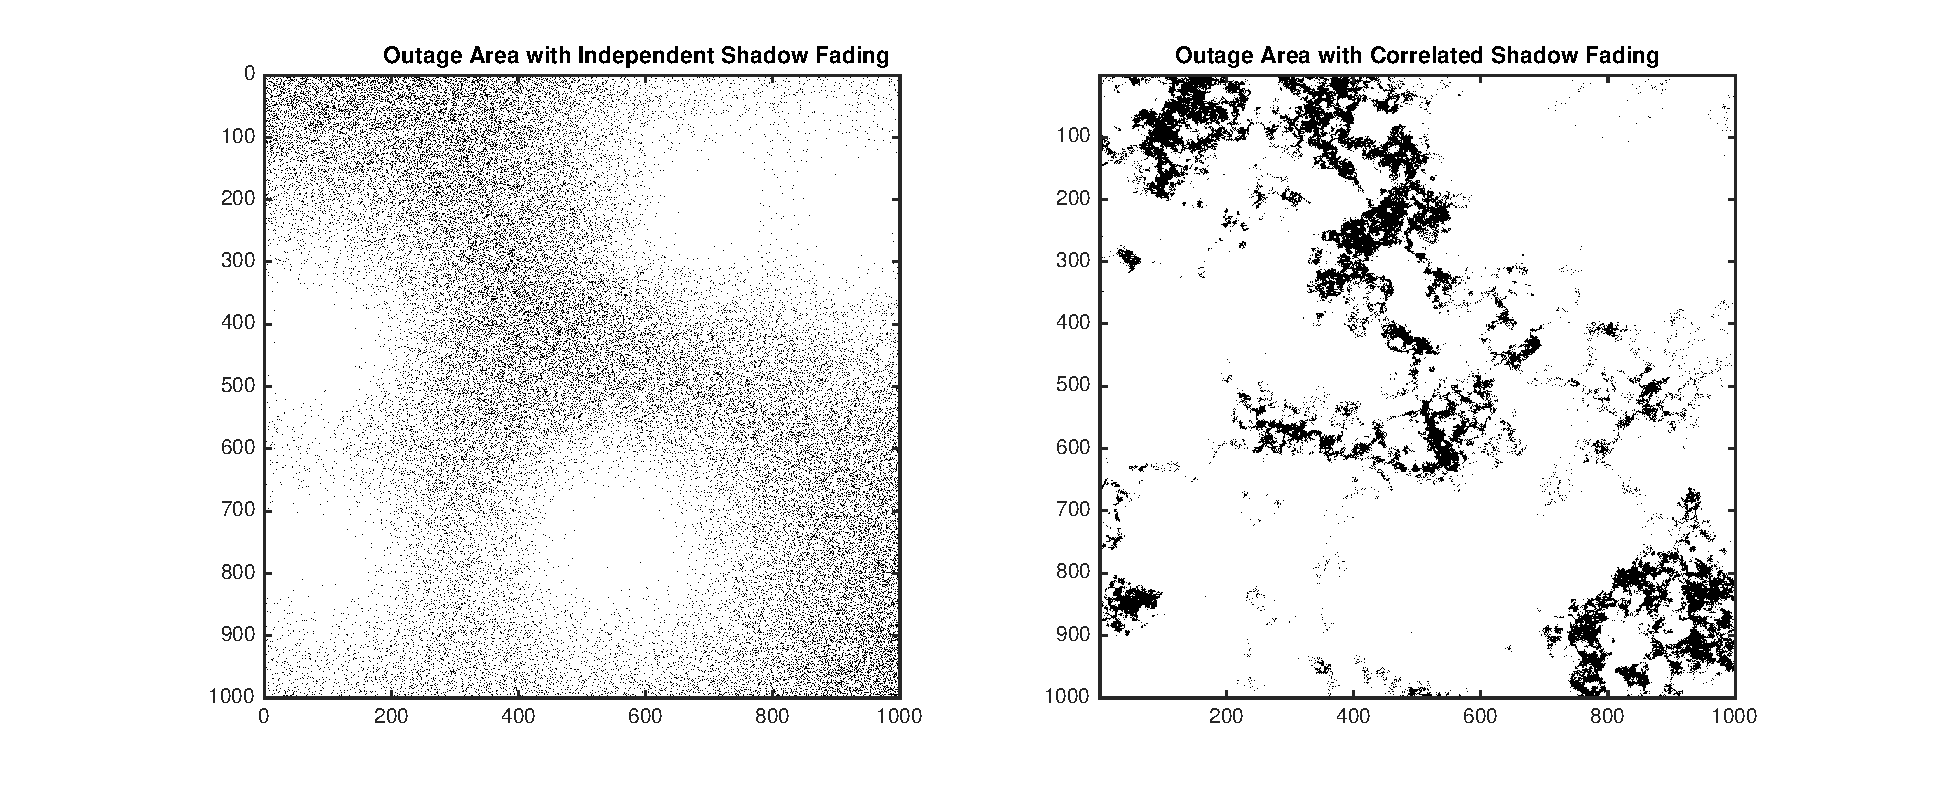
\includegraphics[width=14cm]{outageArea.eps}
 \caption{Correlated outage fields with $\gamma$ (Dark areas are outage areas while white areas are non-outage areas)}
 \label{4:outagefie}
 \end{figure*}


 \section{System Model}
 \label{4:SystemModel}
 In this section, we considered two system models with two different BS deployments: Grid model and Random model.
 \begin{itemize}
 \item Grid model: $\lambda$ BSs are placed on a regular grid deterministically.
 \item Random model: $\lambda$ BSs are placed randomly in a fixed area.
 \end{itemize}
 \begin{figure}
 \centering
 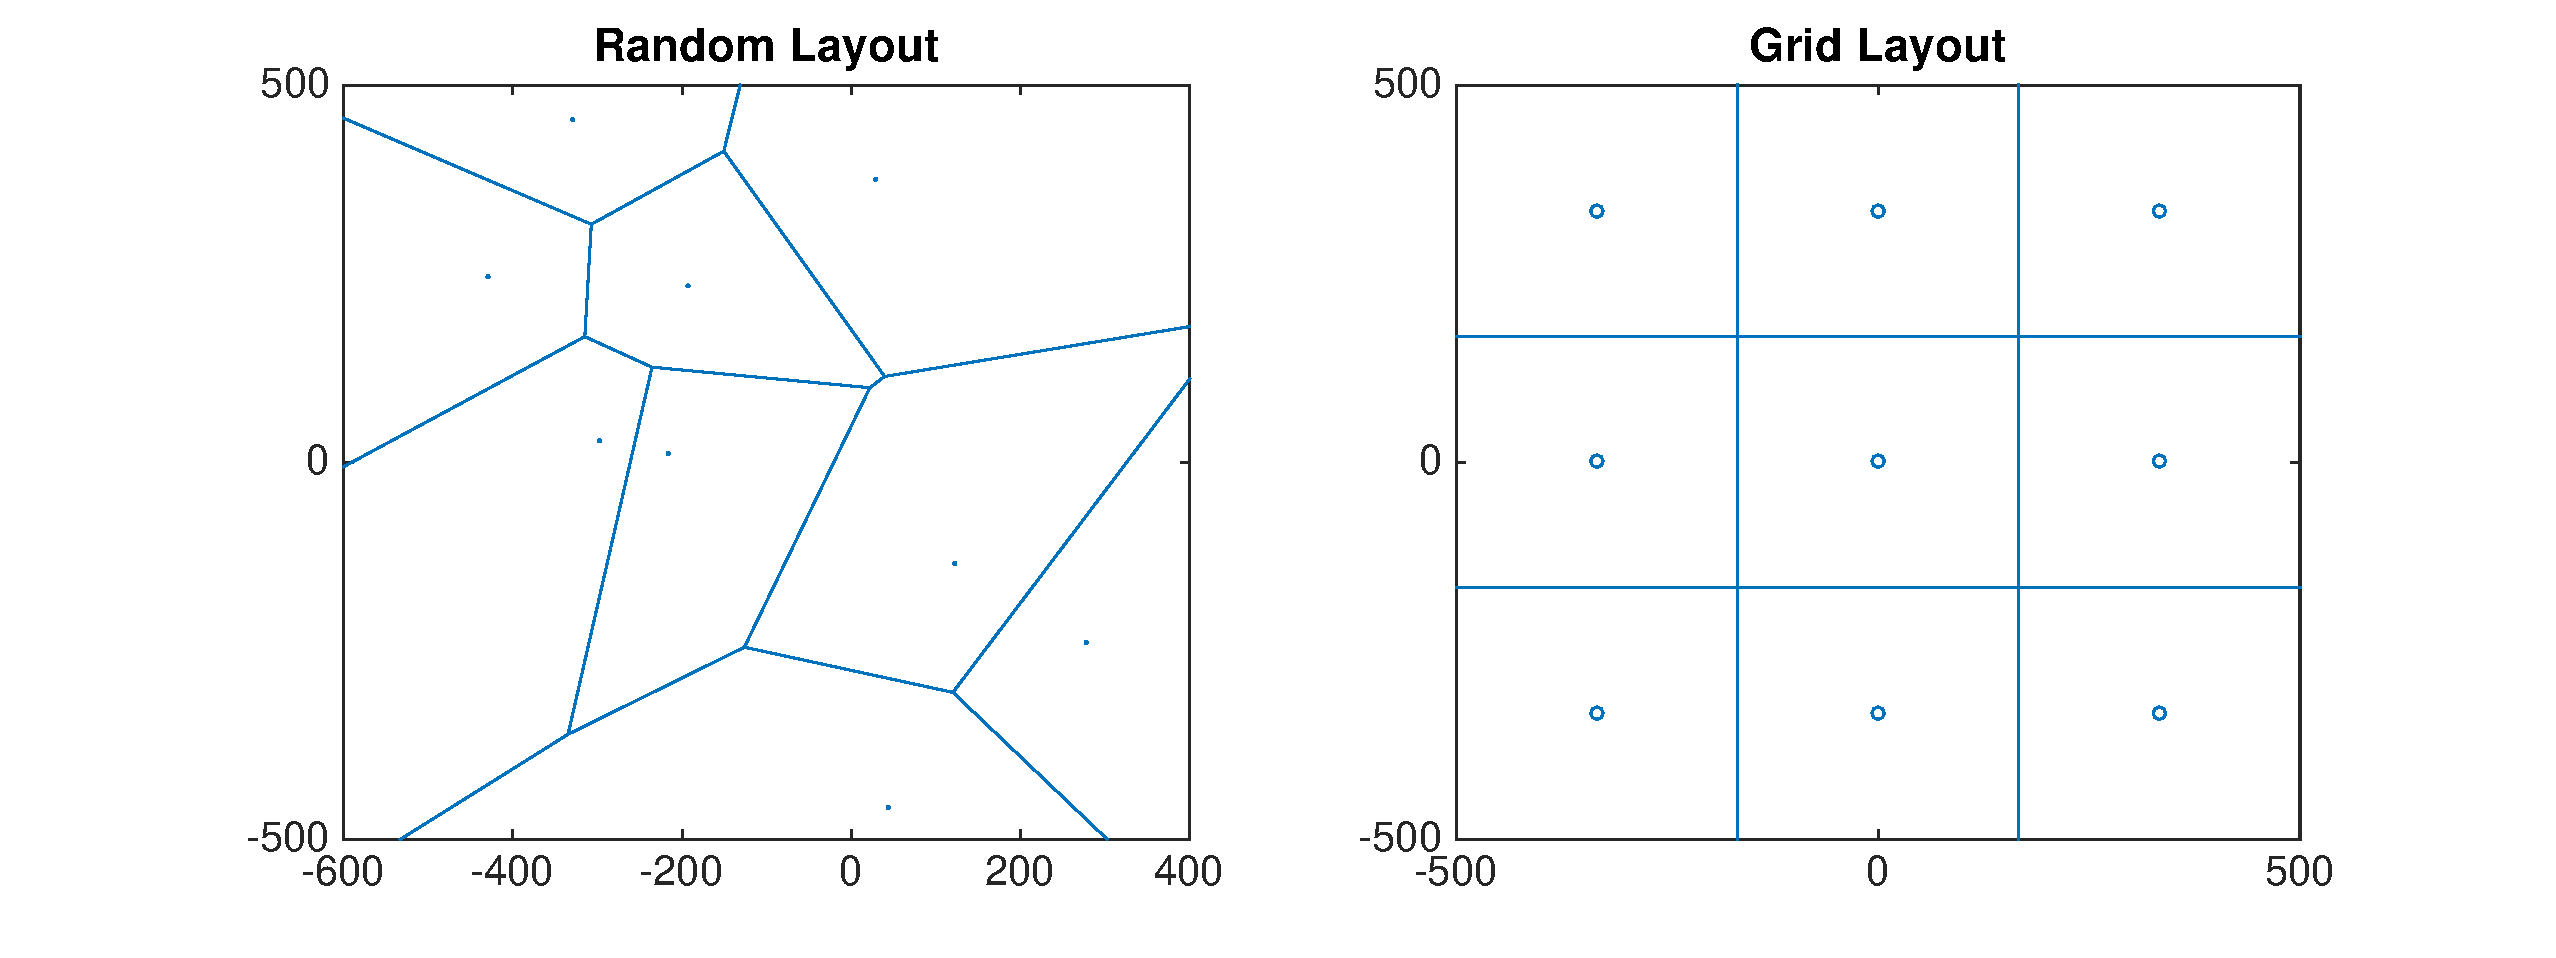
\includegraphics[width=14cm]{systemLayout.eps}
 \caption{Random Layout and Grid Layout with $\lambda = 9$.}
 \label{4:RandomLayout}
 \end{figure}
 % \begin{figure}
 % \centering
 % \includegraphics[width=8cm]{GridLayout.eps}
 % \caption{Grid Base Station Locations}
 % \label{GridLayout}
 % \end{figure}
 Left subfigure of Fig \ref{4:RandomLayout} is an example of a grid model, where cells are in regular square shape with the same size. For the Random model showed in the right subfigure, cells are not guaranteed to be the same shape or same size. Nearest distances between different cells are in a large variation. 


 \section{Outage Probability Analysis}
 \label{4:OutageProb}
 \par Let $\varphi = \{1, 2, \dots, N\}$ denotes the set of all BSs, then the received signal from BS $j$ to the destination user $D$ is given by:
 \begin{equation}
 y_{i\to D} = G_{i\to D}x_{i}+n_{D}.
 \end{equation}
 where $x_{i}$ is the signal transmitted by the source BS and $y_{i\to D}$ is the signal received by the destination user. $n_{D}\sim \mathcal{CN}(0,N_{0})$ is additive white Gaussian noise. $G_{i\to D}$ is the channel gain from source BS to MU including path loss and shadow fading. The end-to-end received $\text{SINR}$ is given in below:
 \begin{equation}
 \text{SINR} \triangleq \frac{P_{i}*G_{i\to D}^{2}}{N_{0}+\sum_{j\in \varphi/i}P_{j}*G_{j\to D}^2},
 \end{equation}
 where $P_{i}$ is the transmitted power of BS $i$. The MU successfully receives the signal if no outage event occurs, i.e., $\log_{2}(1+\text{SINR})\ge R$, where $R$ is the required data rate. From the definition of SINR, no outage event occurs as long as $\text{SINR} > \gamma$, where $\gamma = 2^{R}-1$.

 \par For a particular MU, outage event occurs when its received SINR is less than a threshold to decode the received signal. In our scenario, the probability that the receiver cannot decode signals received from its serving BS is defined as:
 \begin{equation}
 P(out_{i}) = P[\text{SINR}_{i\to D} < \gamma],
 \end{equation}
 We investigate two connection strategies: 
 \begin{itemize}
 \item Nearest BS: MU choose to connect to the nearest BS.
 \item Strongest BS: MU choose to connect to the BS with highest SINR.
 \end{itemize}
 \par In Nearest BS mode, we assume that the MU is served by the nearest BS, then the outage probability will be 
 \begin{equation}
 P_{out} = P_{out_{i}},
 \end{equation} 
 where $i$ is the index of the nearest Base Station. 
 \par In Strongest BS mode, under the assumption that an MS always connecting to the BS which provides the highest SINR, the outage event occurs if no BS can provide high enough SINR to the receiver. Based on this assumption we have:
 \begin{equation}
 P_{out} = \max_{i = 1,\cdots,N} P[\text{SINR}_{i\to D}<\gamma].
 \end{equation}
 The probability density function (pdf) of shadow fading $S$ given $L$ correlated fading branches is
 \begin{equation}
 \begin{split}
 f_{\mathbf{S}}(\mathbf{s}) = &\frac{\lambda^{L}}{\sqrt{2\pi}|\mathbf{K}_{L\times L}|^{1/2}\prod_{i=1}^{L}s_{i}}\\
 &\cdot\exp(-\frac{1}{2}(10\log_{10}\mathbf{s}-\boldsymbol{\mu})^{T}\mathbf{K}_{L\times L}^{-1}(10\log_{10}\mathbf{s}-\boldsymbol{\mu})),
 \end{split}
 \end{equation}
 where $\lambda = 10/\ln10$ and $\boldsymbol{\mu}$ is the average shadow fading which is normally $0$. $\mathbf{K}_{L\times L}$ is the correlation matrix which is defined in \eqref{correlationmatrix}. Let $\theta_{i} = \frac{10\log_{10}s_{i}-\mu_{i}}{\sqrt{2}\sigma_{i}}$, and doing a change of variables gives us the pdf of $\mathbf{\Theta}$ as follows:
 \begin{equation}
 f_{\mathbf{\Theta}}(\boldsymbol{\theta}) = \frac{1}{\pi^(L/2)|\mathbf{\Sigma}|^{1/2}}\exp(-\mathbf{\Theta}^{T}\mathbf{\Sigma}^{-1}\mathbf{\Theta}),
 \end{equation}
 where $\mathbf{\Sigma}$ is the correlation coefficient matrix which is
 \begin{equation}
 \left[\begin{array}{cccc}
 1 & h_{1,2} & \cdots & h_{1,L}\\
 \vdots & \ddots & \ddots & \vdots\\
 h_{L,1} & h_{L,2} & \cdots & 1\\
 \end{array}\right].
 \end{equation}
 Since $\text{SINR}_{i\to D}=PL_{i\to D}+S_{i}-N_{0}-\sum_{j\in\varphi/i}(PL_{j\to D} + S_{j})$ in dB, $\text{SINR}_{i\to D}<\gamma$ means
 \begin{equation}
 S_{i} - \sum_{j\in\varphi/i}S_{j}<\gamma -PL_{i\to D} + \sum_{j\in\varphi/i}PL_{j\to D} + N_{0},
 \end{equation}
 where $\varphi$ denotes the set of all BSs.
 Then the outage probability can be written as:
 \begin{equation}
 \label{4:outprob}
 P_{out} = \underbrace{\int_{-\infty}^{+\infty}\cdots\int_{-\infty}^{+\infty}}_{i =1,\cdots,N} g(PL_{i}S_{i} - \gamma\sum_{j\in\varphi/i}PL_{j}S_{j})f(\mathbf{s})d\mathbf{s}.
 \end{equation}
 where $\mathbf{s}$ is the correlated shadow fading experienced by all BSs, $g(PL_{i}S_{i} - \gamma\sum_{j\in\varphi/i}PL_{j}S_{j})$ is a step function defined in (\ref{4:stepfunction}). 
  \begin{figure}[!t]
 % ensure that we have normalsize text
 \normalsize
 % Store the current equation number.
 % \setcounter{MYtempeqncnt}{\value{equation}}
 % % Set the equation number to one less than the one
 % % desired for the first equation here.
 % % The value here will have to changed if equations
 % % are added or removed prior to the place these
 % % equations are referenced in the main text.

 \begin{equation}
 \label{4:stepfunction}
 g(PL_{i}S_{i} - \gamma\sum_{j\in\varphi/i}PL_{j}S_{j}) = \{\begin{array}{cc}
                1, &  \text{  when }PL_{i}S_{i} - \gamma\sum_{j\in\varphi/i}PL_{j}S_{j} <\frac{\gamma N_{0}}{P}\\
                0, & \text{  when }PL_{i}S_{i} - \gamma\sum_{j\in\varphi/i}PL_{j}S_{j} >\frac{\gamma N_{0}}{P}
              \end{array}.
 \end{equation}
 % Restore the current equation number.
 % \setcounter{equation}{\value{MYtempeqncnt}}
 % IEEE uses as a separator
 \hrulefill
 % The spacer can be tweaked to stop underfull vboxes.
 \vspace*{4pt}
 \end{figure}

 \section{Simulation Results}
 \label{4:SimuProb}
 \par In this section, we will present simulation setup and results. Firstly, we run simulations to compare the outage probability of the two different network topologies: Grid model and Random model. Secondly, SINR distribution and outage probability of Random model given different BS densities are investigated. Two scenarios are considered: MU connecting to the nearest BS and MU connecting to the BS providing highest SINR. At the end, the outage duration distribution are simulated and discussed given different BS densities. The simulation parameters are presented in Table \ref{SystemConfig2}. 
 \begin{table}
 \centering
 \caption{\label{SystemConfig2}Simulation Configuration Parameters}

 \begin{tabular}{|c|c|}

 \hline
 Study Area & $1000m\times 1000m$\\
 \hline
 BS Densities & $3, 10, 50, 100, 200, 300, 500$\\
 \hline
 Path Loss Exponent & $4$\\
 \hline
 BS Transmission Power & $P: 40dbm$\\
 \hline
 SNR Requirement & $-5dB$\\
 \hline
 De-Correlation Distance & $20m, 200m$\\
 \hline
 \end{tabular}

 \end{table}

 \par Figure \ref{4:cdf1} shows the Cumulative Distribution Function (CDF) of SINR when MU is connecting to the nearest BS. The de-correlation distance of the correlated shadow fading is $20m$. The figure suggests that Grid model outperforms the Random model, which is consistent with findings in \cite{andrews2011tractable}. Figure \ref{4:outage1} shows the outage probability with SINR threshold being $-5dB$. The outage probability of Grid Layout (blue) is lower than that of the Random Layout (yellow). In next section, we will focus on the Random model which is more realistic than Grid model.
 \begin{figure}
 \centering
 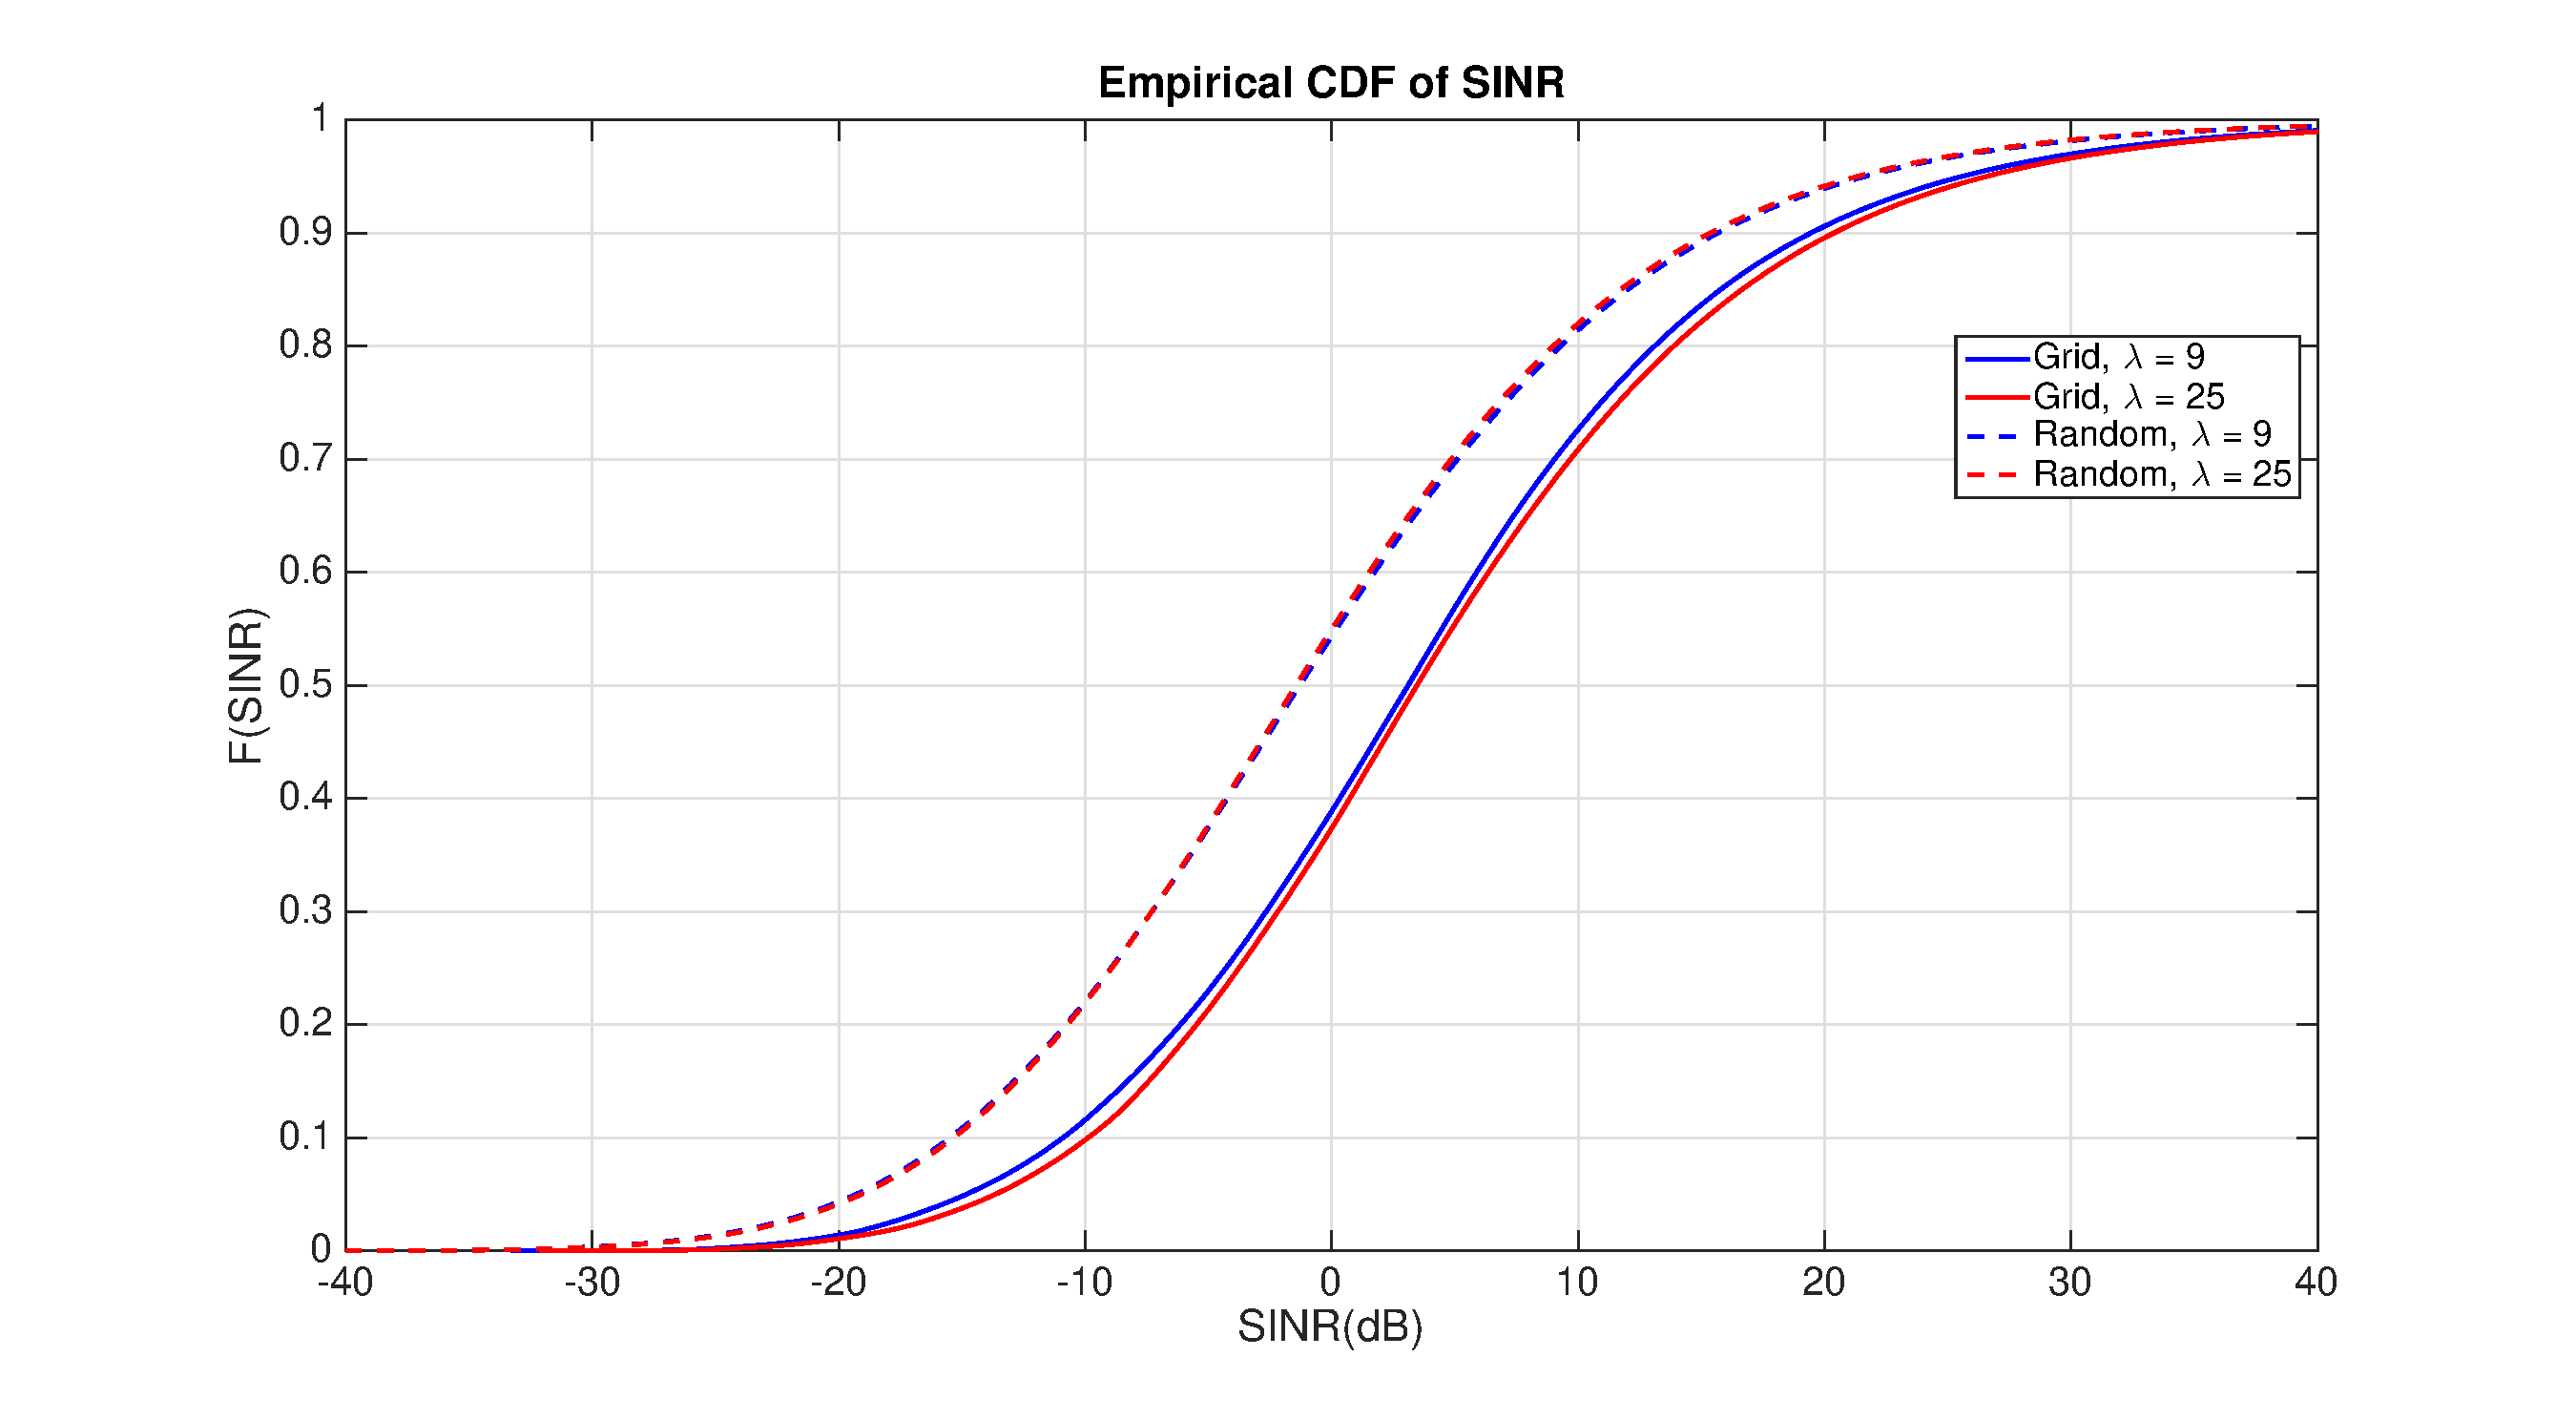
\includegraphics[width=10cm]{GridVSRandom.eps}
 \caption{CDF of SINR given Grid Layout and Random Layout (De-Correlation Distance: $20m$)}
 \label{4:cdf1}
 \end{figure}
 \begin{figure}
 \centering
 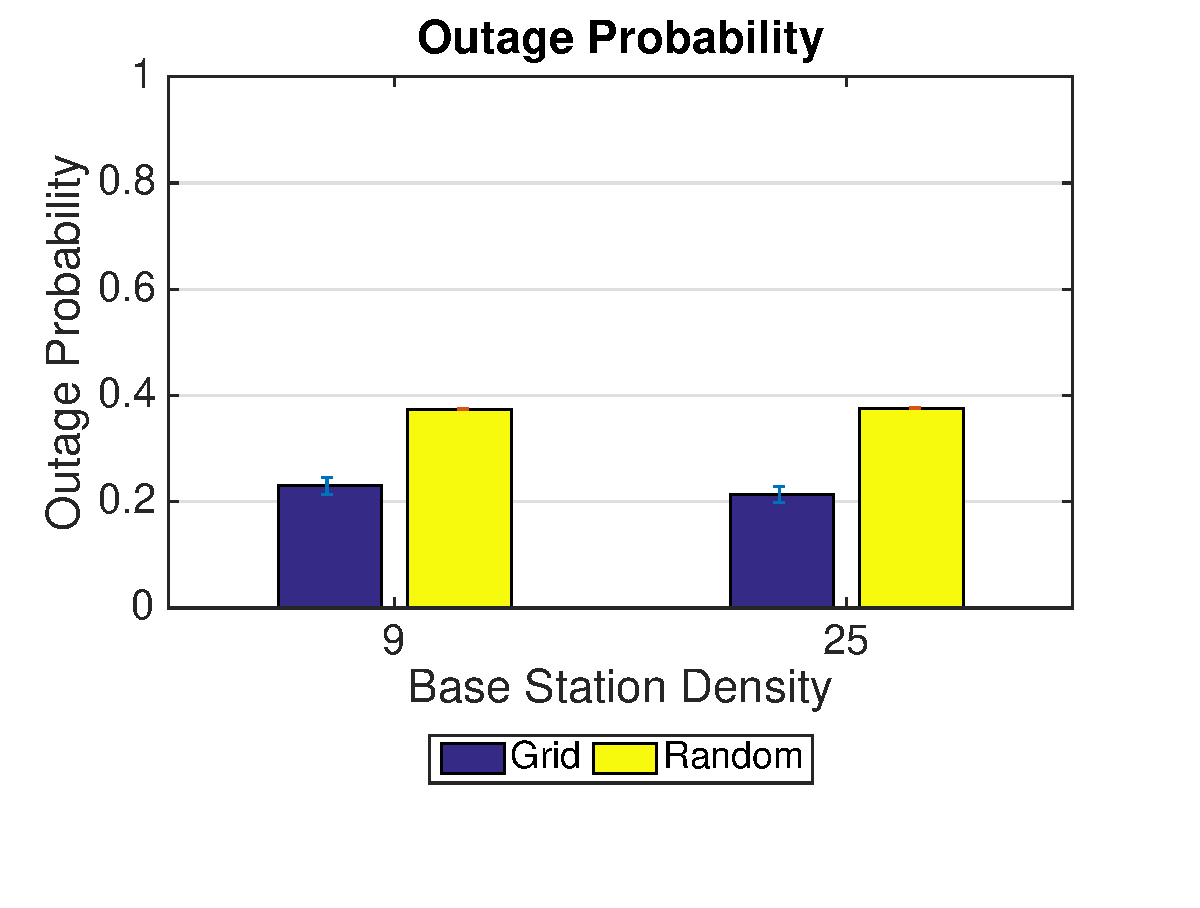
\includegraphics[width=10cm]{OutageProbGridVSRandom.eps}
 \caption{Outage Probability given Grid Layout and Random Layout (De-Correlation Distance: $20m$)}
 \label{4:outage1}
 \end{figure}


 \begin{figure}
 \centering
 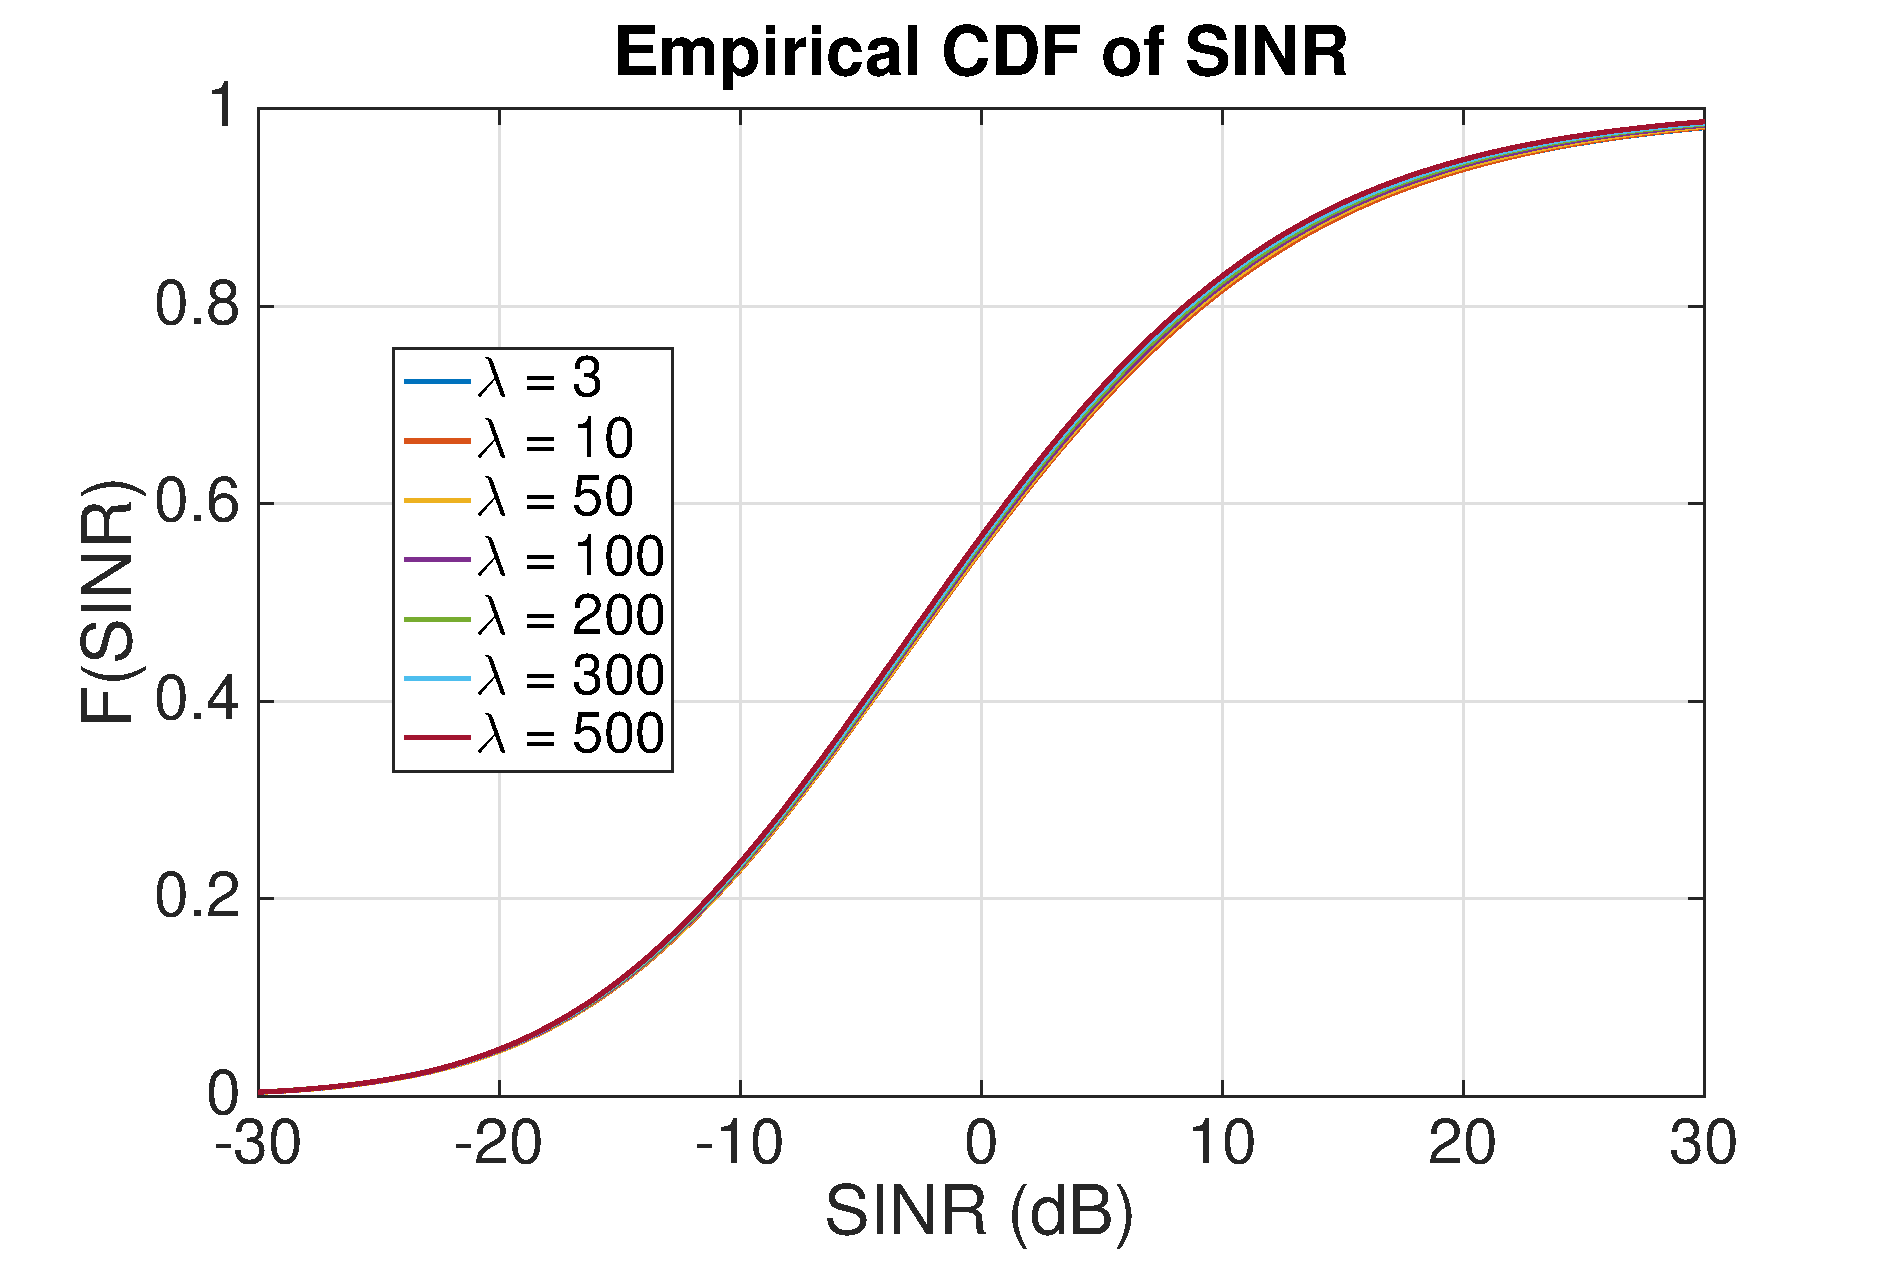
\includegraphics[width=10cm]{NBMax1000OutageProbCDFiid.eps}
 \caption{CDF of SINR of MU when connecting to the nearest BS. i.i.d. Shadow Fading}
 \label{4:Mode1}
 \end{figure}
 \begin{figure}
 \centering
 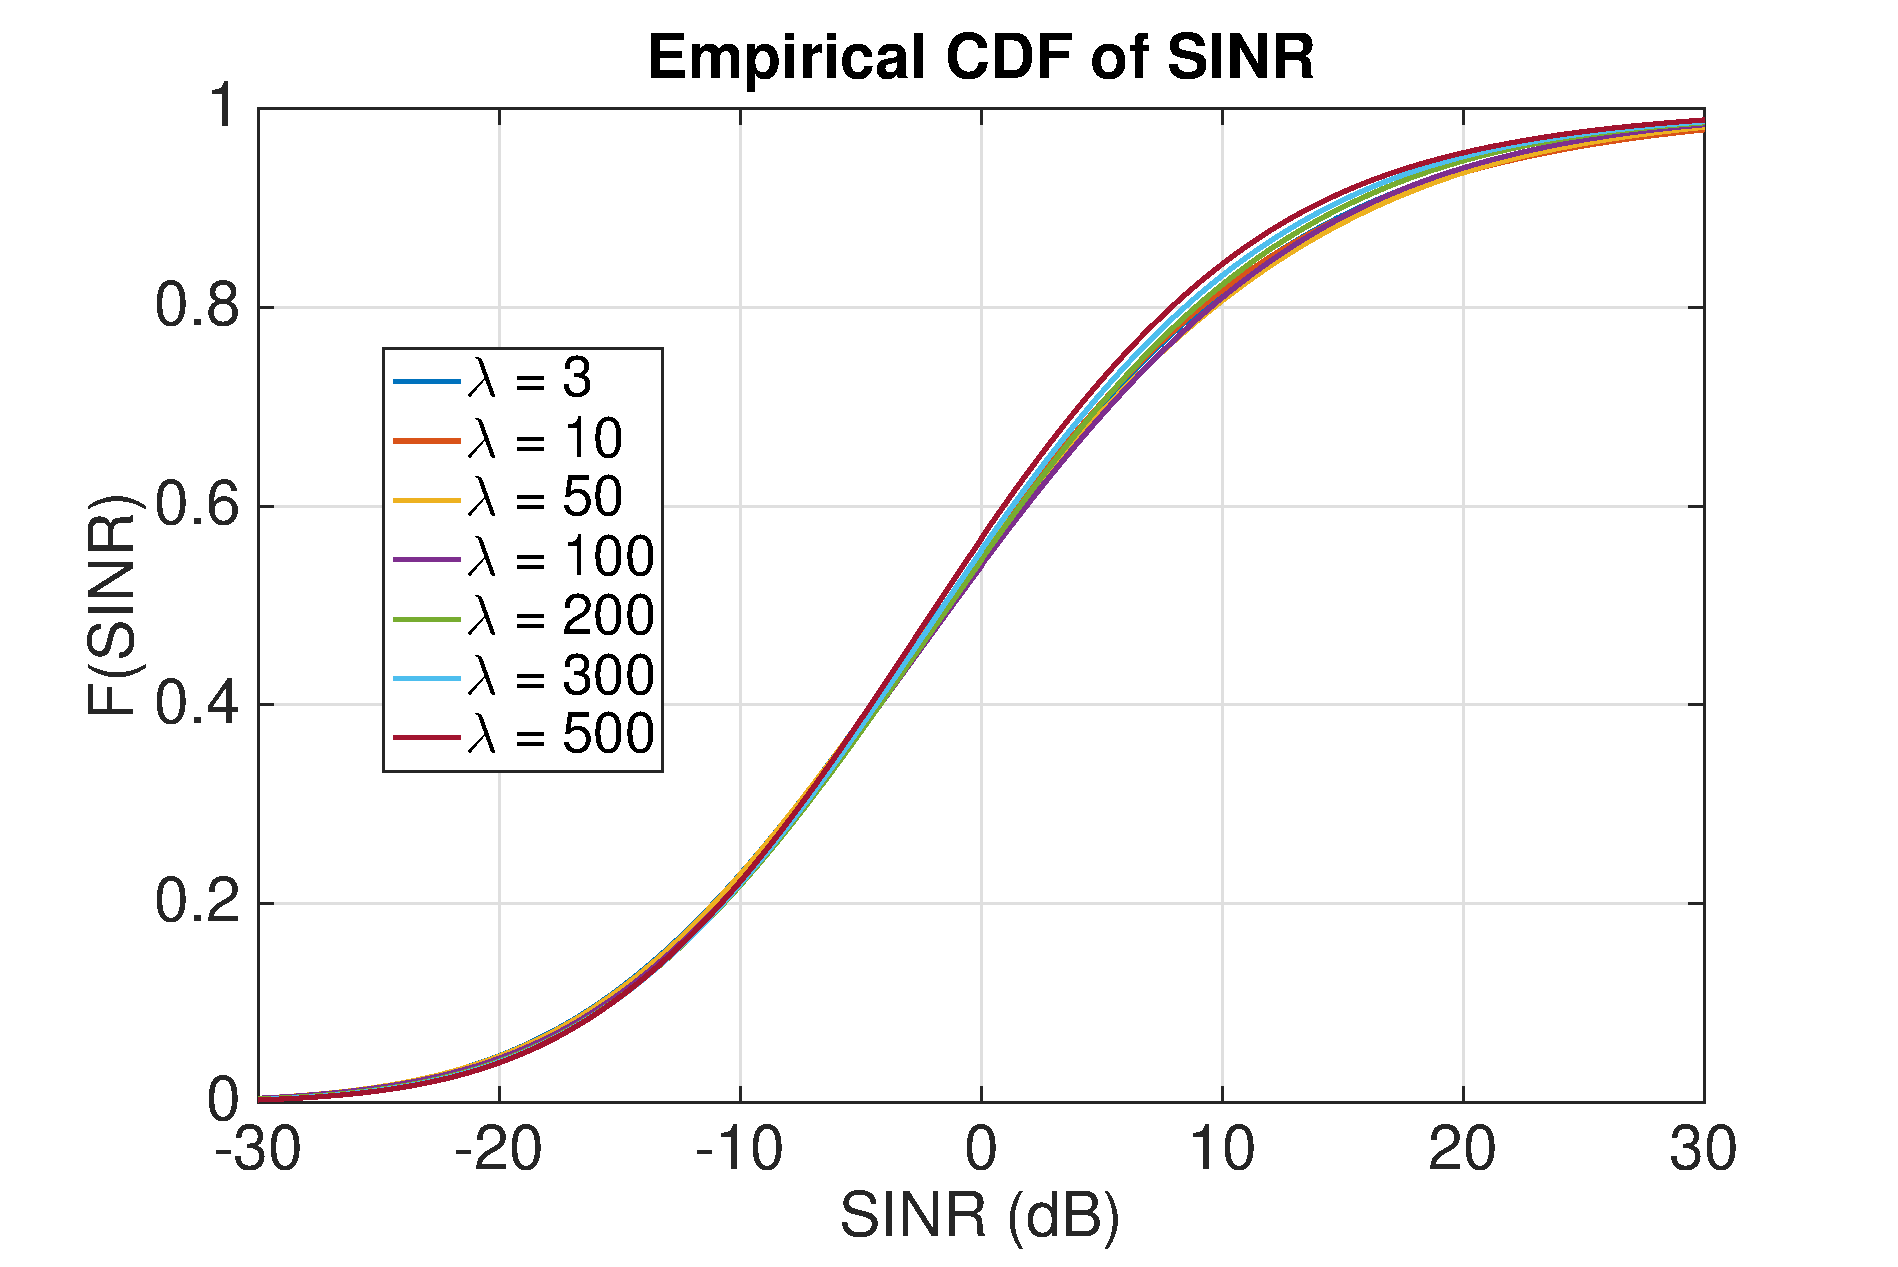
\includegraphics[width=10cm]{NBMax1000OutageProbCDFDeCorr20.eps}
 \caption{CDF of SINR of MU when connecting to the nearest BS. De-Correlation Distance: 20m}
 \label{4:Mode2}
 \end{figure}
 \begin{figure}
 \centering
 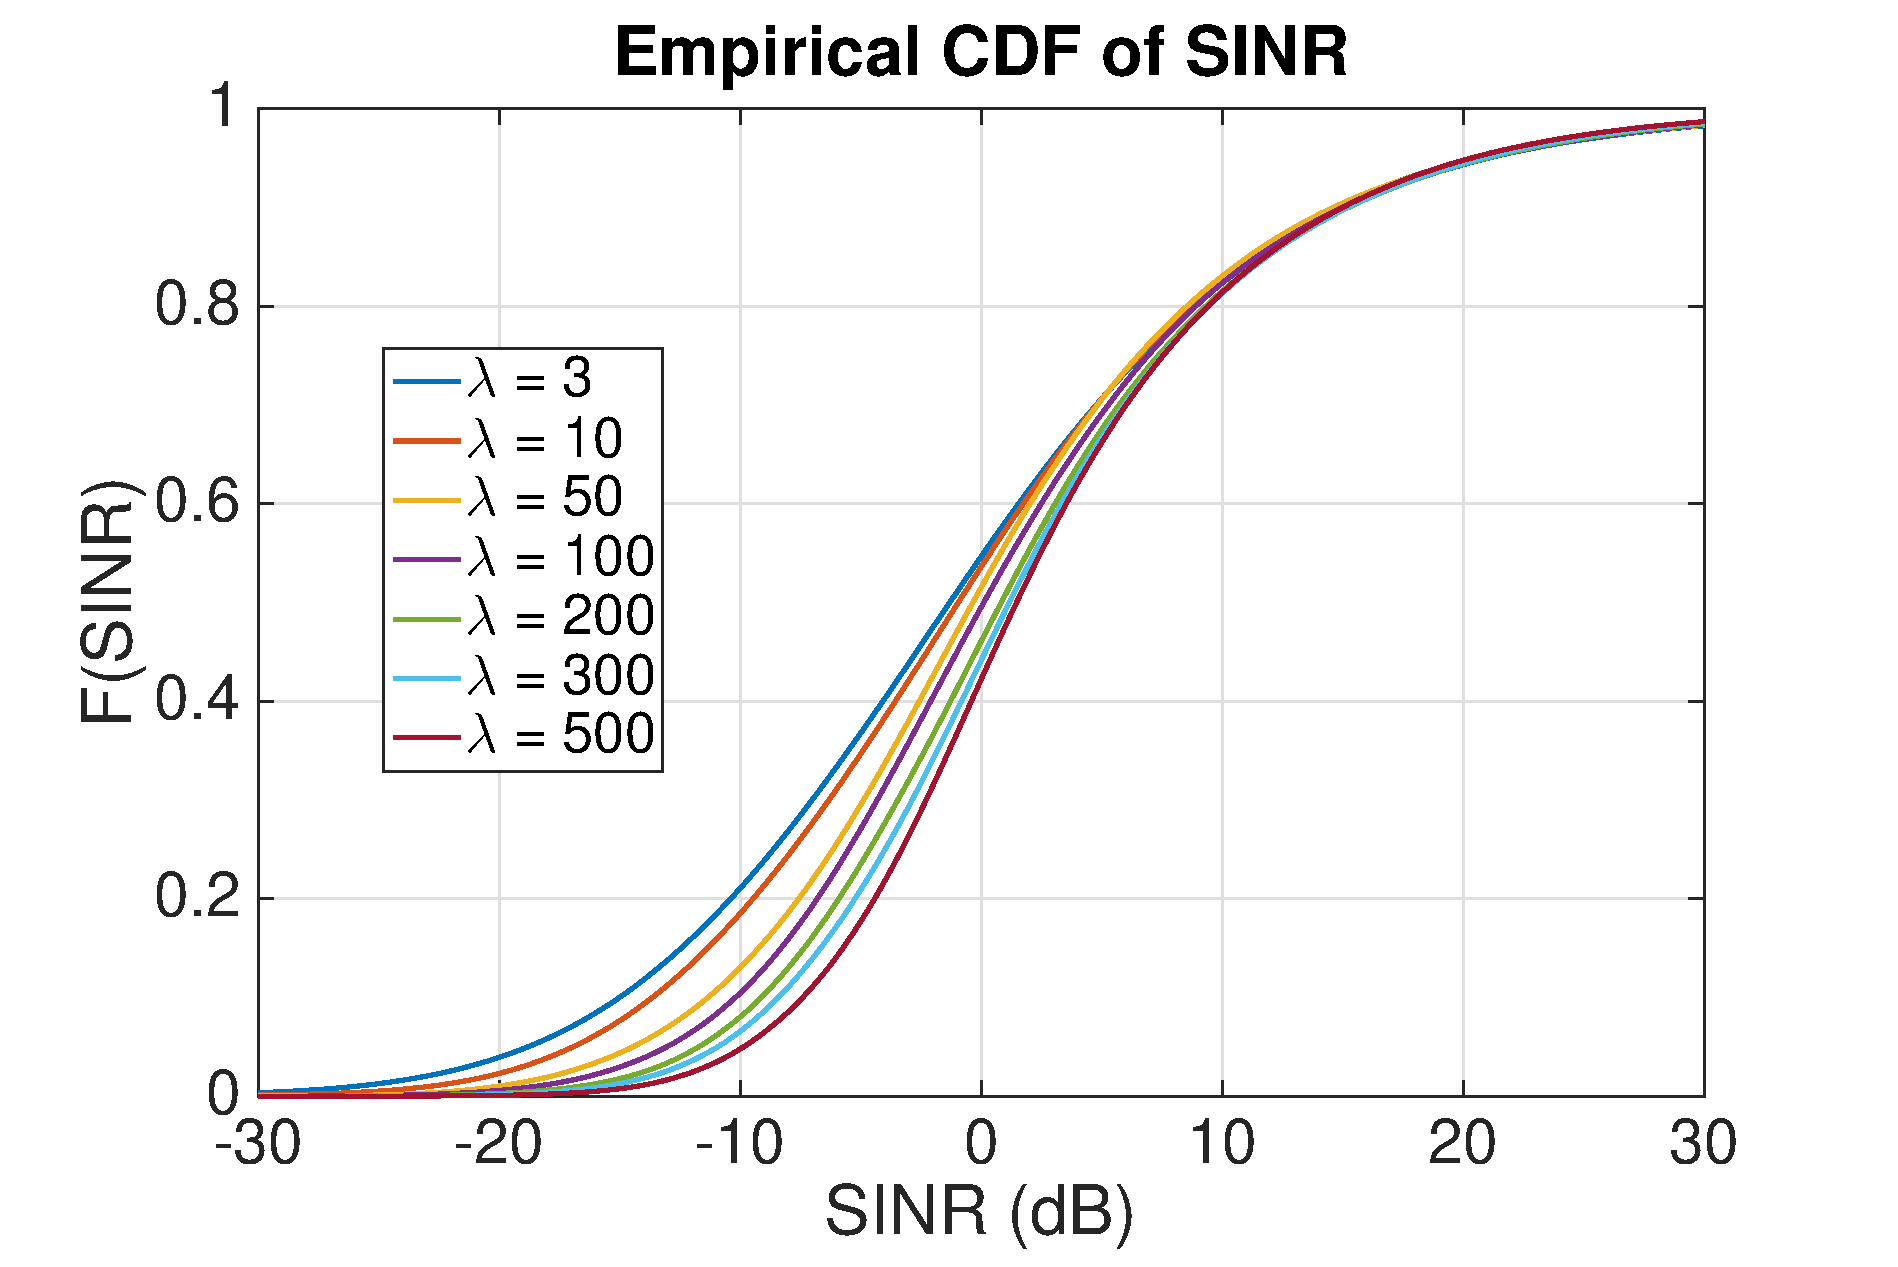
\includegraphics[width=10cm]{NBMax1000OutageProbCDFDeCorr200.eps}
 \caption{CDF of SINR of MU when connecting to the nearest BS. De-Correlation Distance: 200m}
 \label{4:Mode3}
 \end{figure}


 \begin{figure}
 \centering
 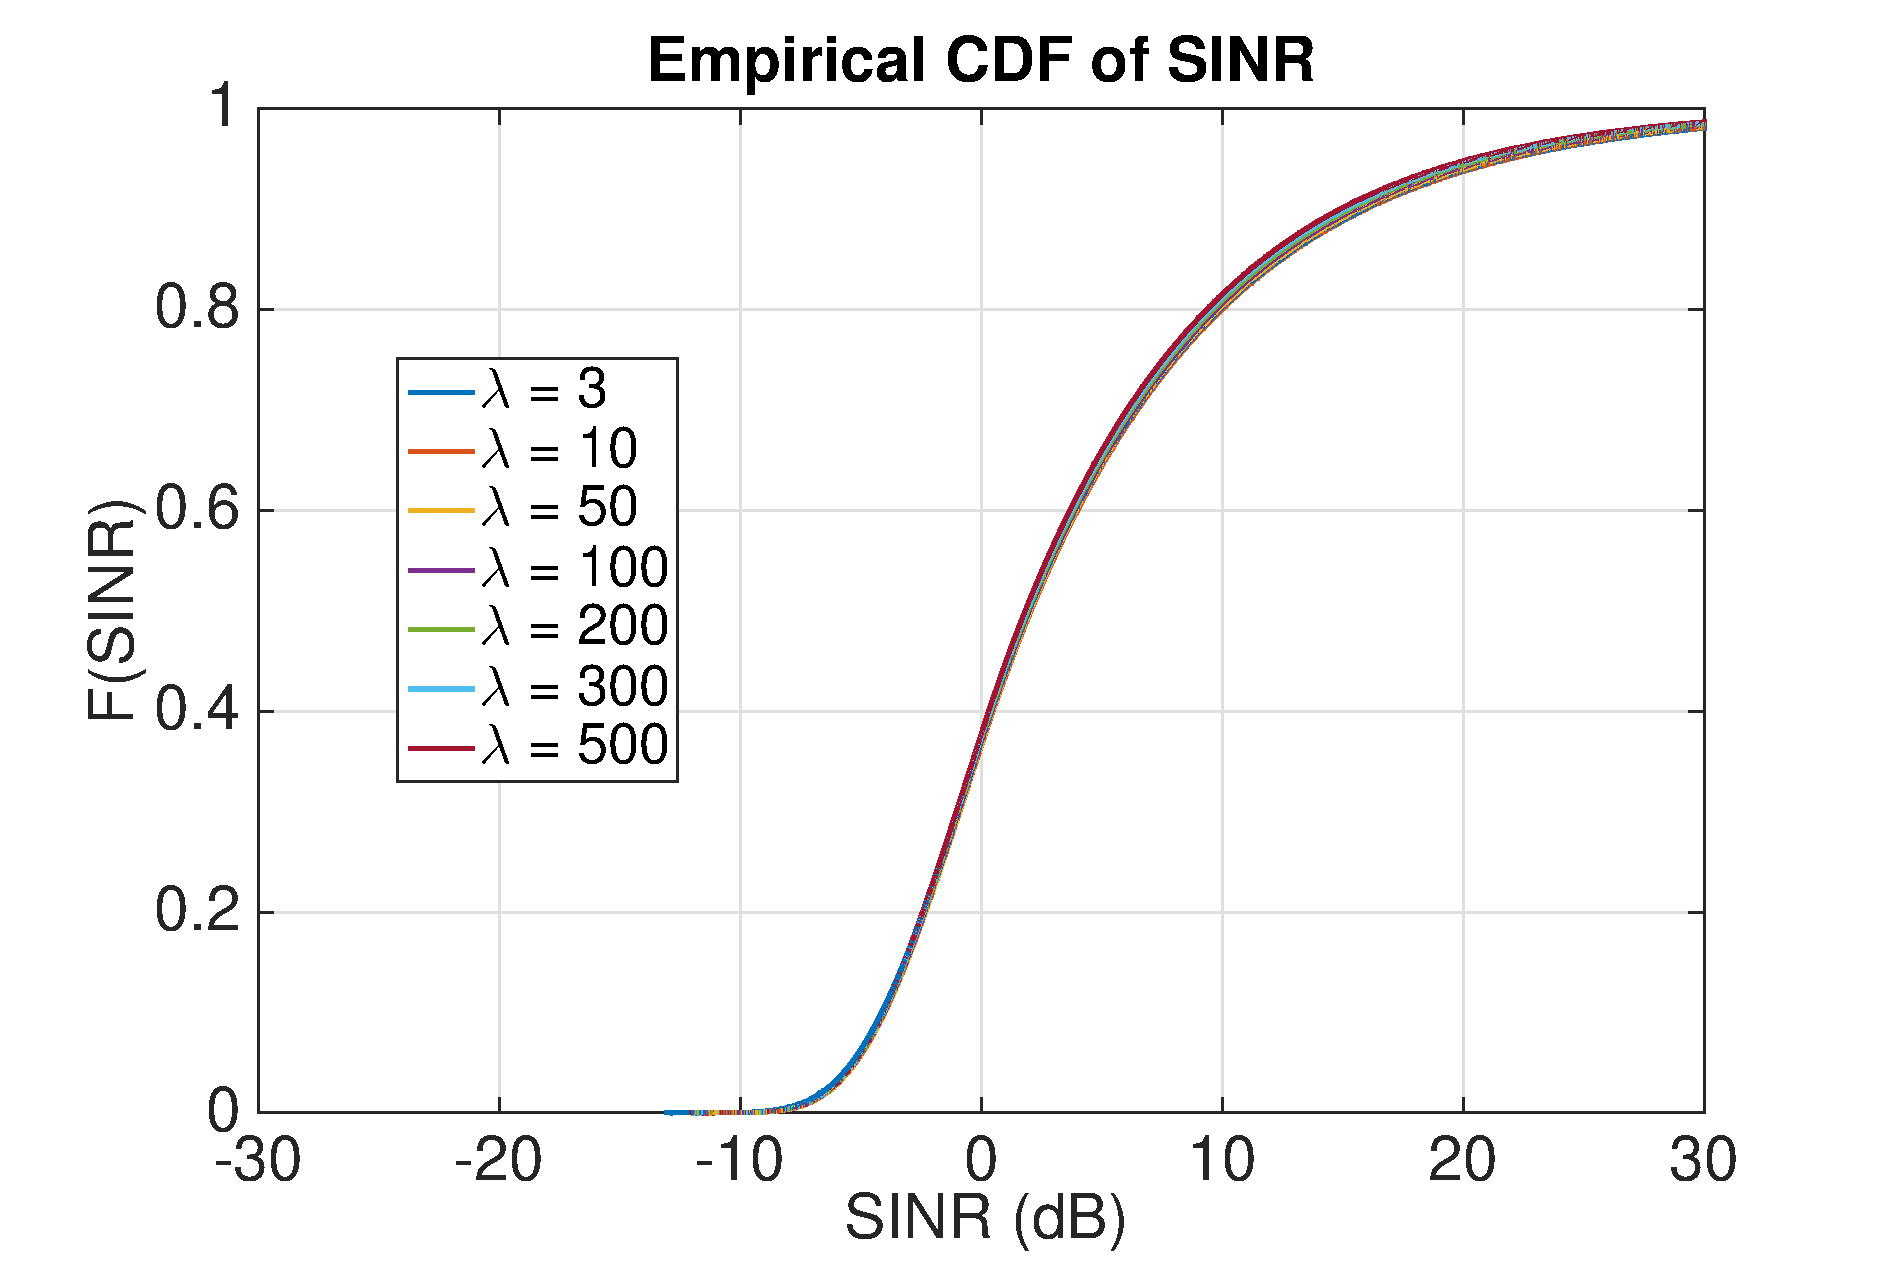
\includegraphics[width=10cm]{MaxMax1000OutageProbCDFiid.eps}
 \caption{CDF of SINR of MU when connecting to the strongest BS. i.i.d. Shadow Fading}
 \label{4:Mode12}
 \end{figure}
 \begin{figure}
 \centering
 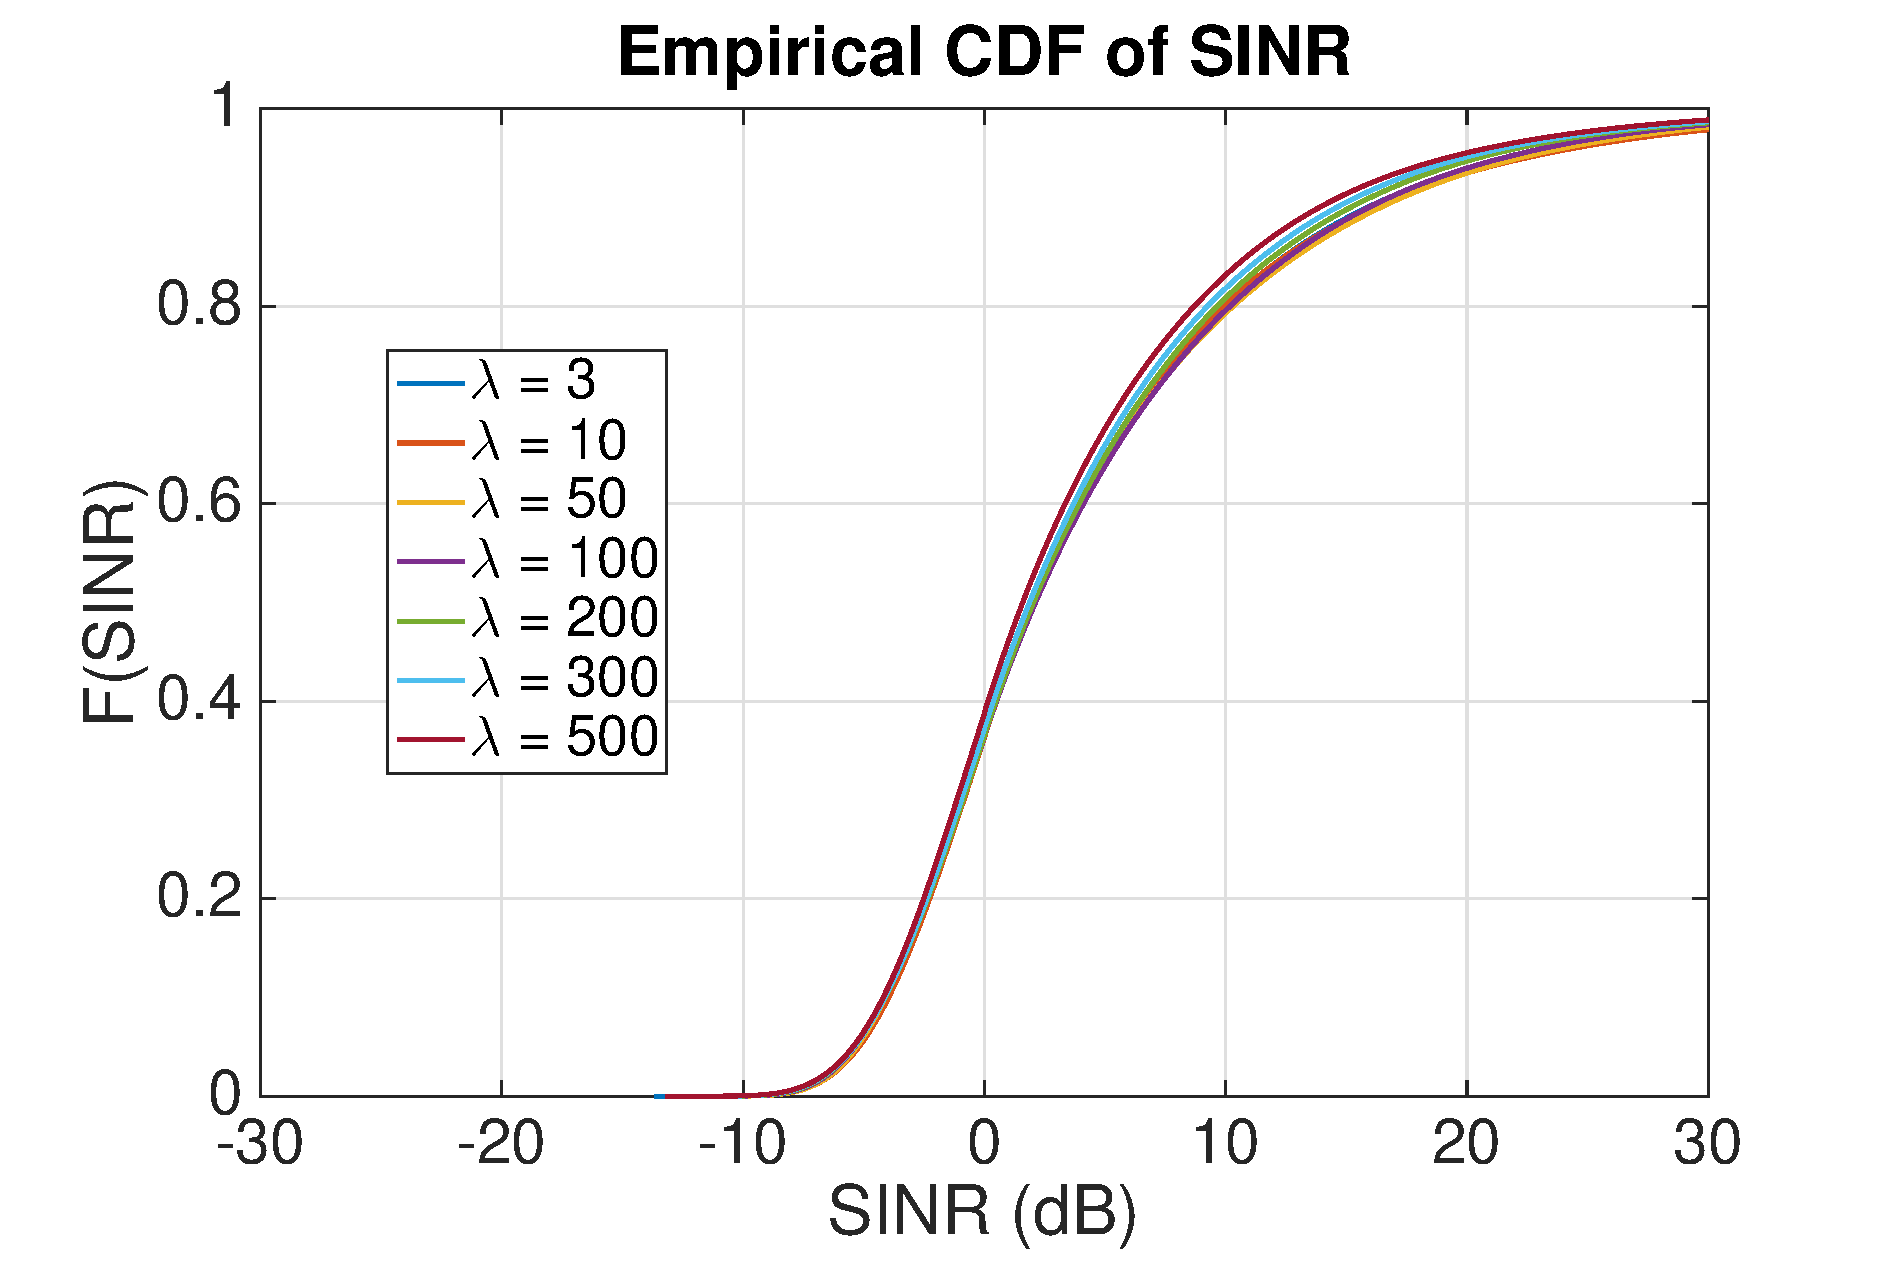
\includegraphics[width=10cm]{MaxMax1000OutageProbCDFDeCorr20.eps}
 \caption{CDF of SINR of MU when connecting to the strongest BS. De-Correlation Distance: 20m}
 \label{4:Mode22}
 \end{figure}
 \begin{figure}
 \centering
 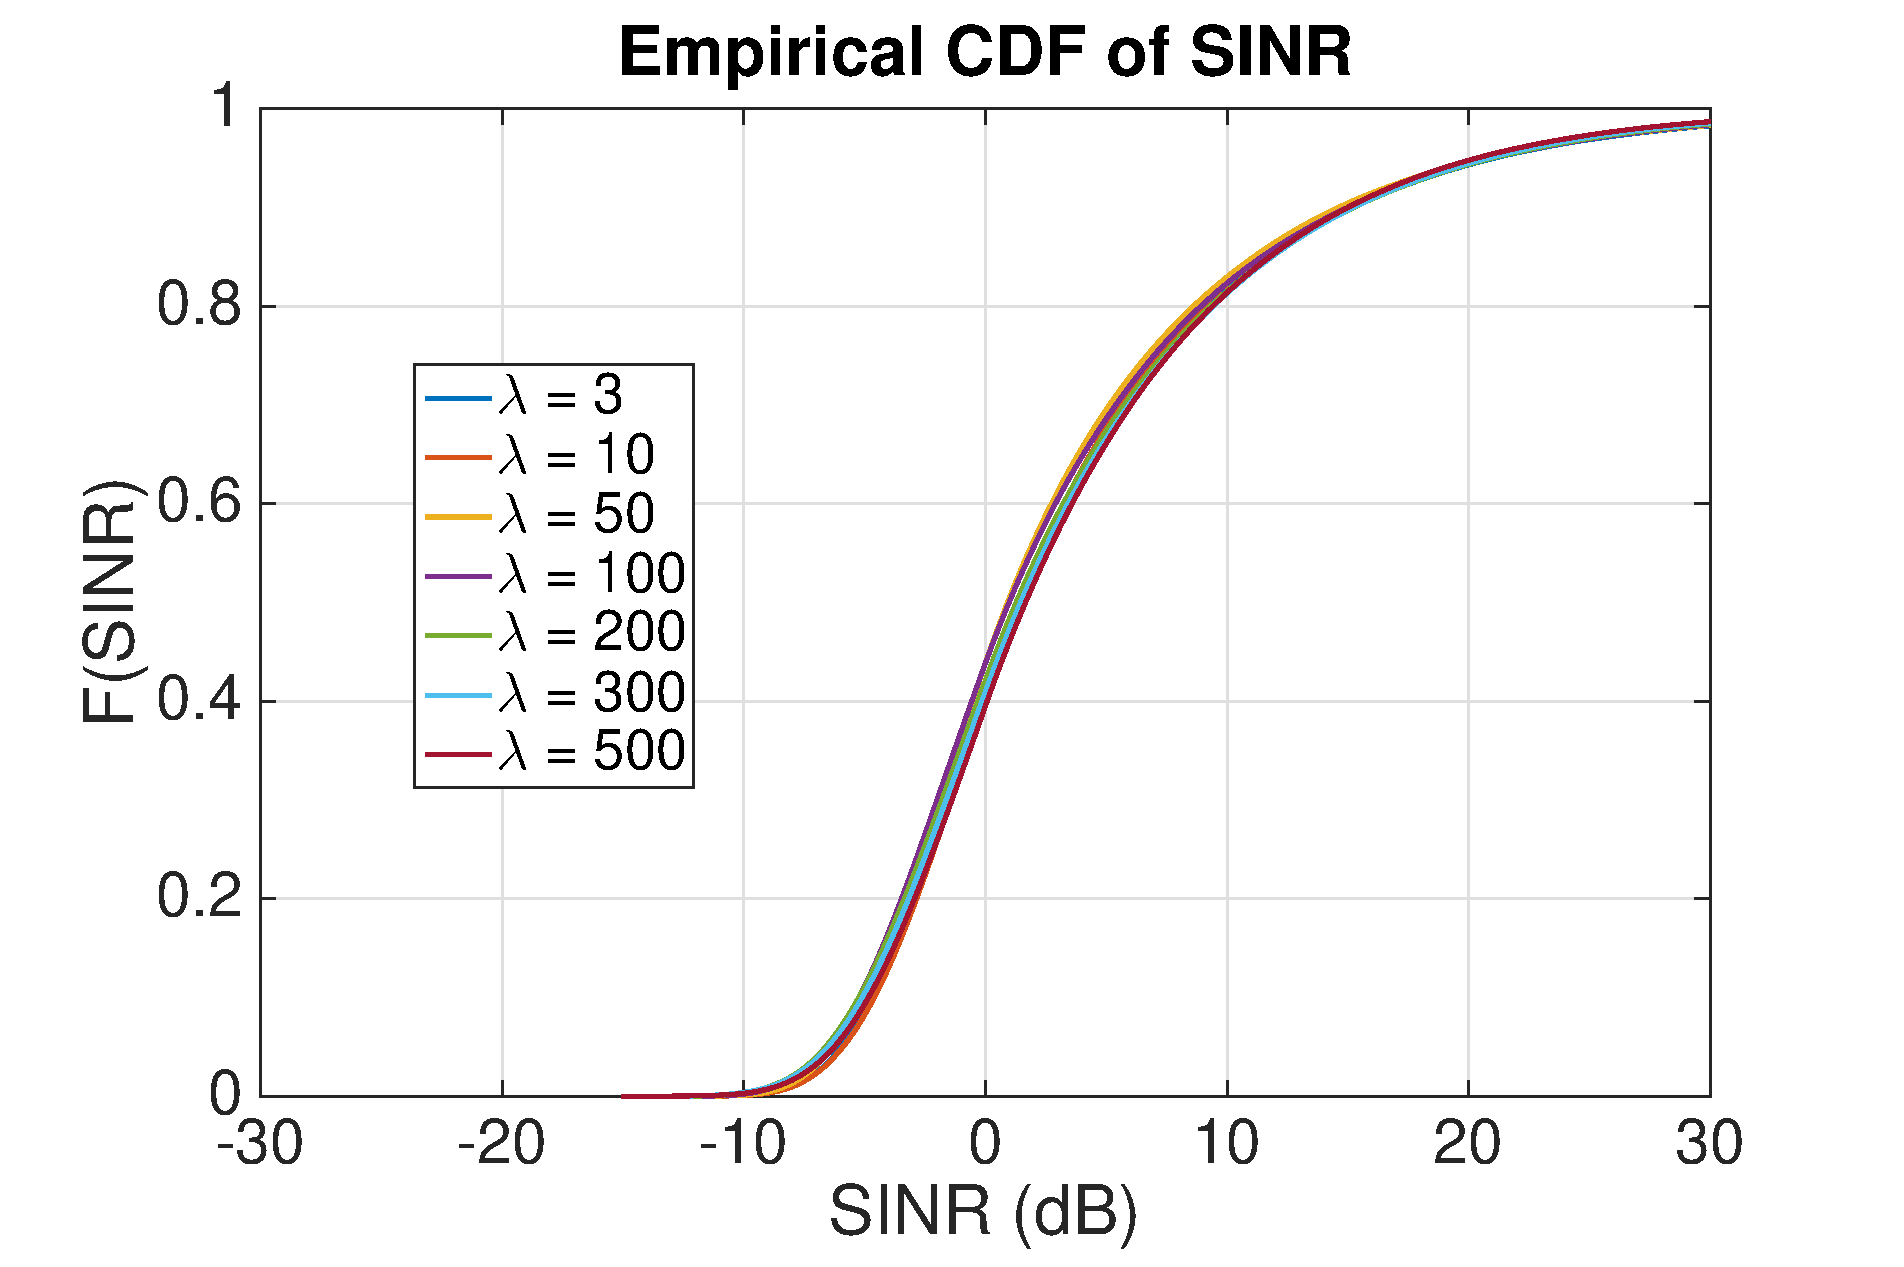
\includegraphics[width=10cm]{MaxMax1000OutageProbCDFDeCorr200.eps}
 \caption{CDF of SINR of MU when connecting to the strongest BS. De-Correlation Distance: 200m}
 \label{4:Mode32}
 \end{figure}

 \par For Random model, SINR distribution and outage probability of different BS densities are investigated for both Nearest BS mode and Strongest BS mode. Simulations are run for independent shadow fading and correlated shadow fading. CDF curves of SINR are generated and outage probability given SINR threshold being $-5dB$ are presented for increasing BS densities. Figure \ref{4:Mode1}, \ref{4:Mode2} and \ref{4:Mode3} shows the SINR of MU when connecting to the nearest BS. From Figure \ref{4:Mode1} and \ref{4:Mode2} we can see that the CDF curves are overlapping each other, which means increasing BS density does not change the CDF of SINR. From this we can conclude that when the shadow fading is independent or the de-correlation distance of the correlated shadow fading is small, increasing BS will not improve the system performance in terms of reducing outage probability. Figure \ref{4:Mode3}  illustrates that when increasing BS density, CDF of SINR improves (curve moves toward the bottom-right corner). This indicates that when de-correlation distance is large, increasing BS density will result in better system performance by reducing outage probability. Figure \ref{fig: outprob1} shows the outage probability of different correlated shadow fading models and different BS densities when SINR threshold is set to $-5dB$. Blue and green bars suggest that increasing BS density will not decrease outage probability when shadow fading is independent or correlated with $20m$ de-correlation distance. Yellow bars suggest that when the de-correlation distance is $200m$, increasing BS density will reduce outage probability. For example, when BS density is $3$, the outage probability is around $38\%$. Increasing BS density to $500$, the outage probability decreases to $18\%$. All above simulation results suggest that when de-correlation distance is relatively large and the MU is connecting to the nearest BS, increasing BS density will reduce outage probability and improve system performance.



 \begin{figure}
 \centering
 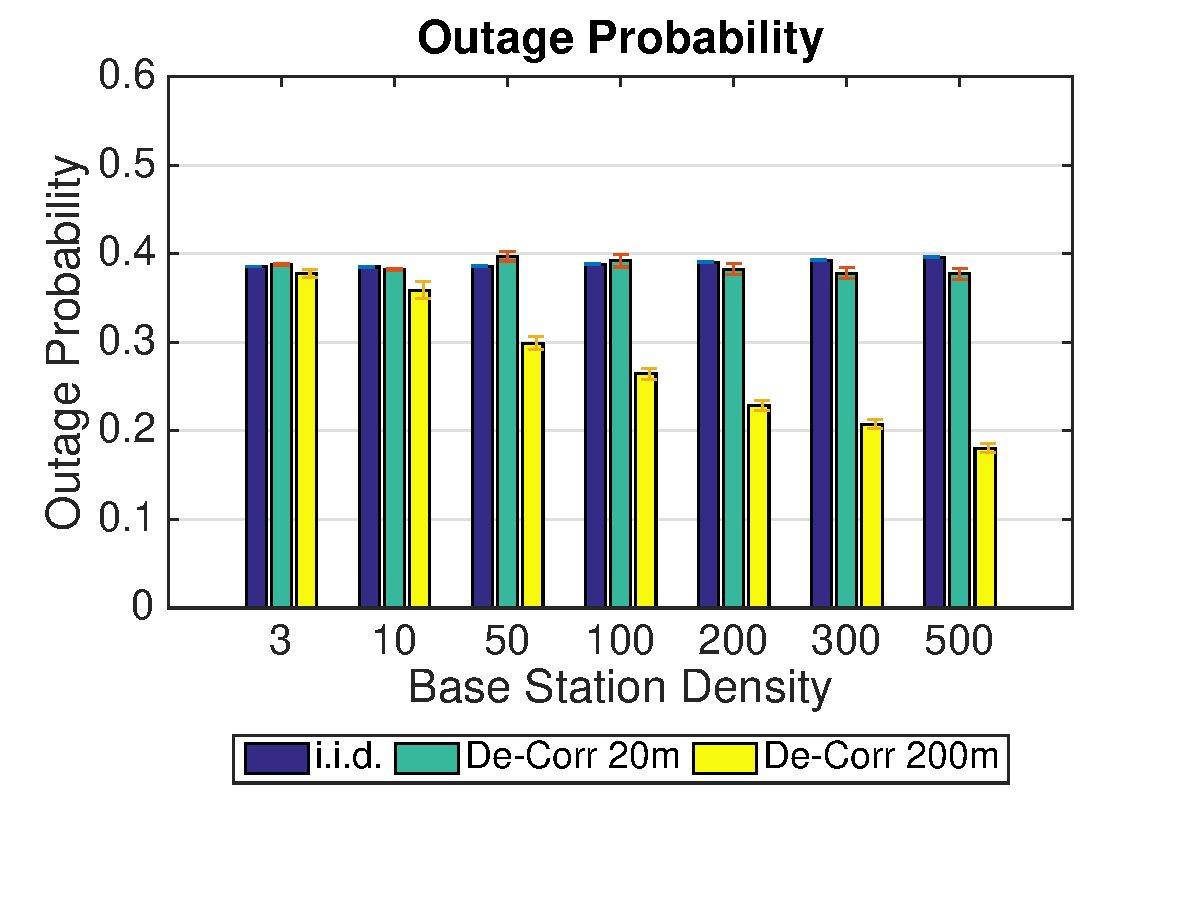
\includegraphics[width=10cm]{NBMax1000OutageProbThresh-5iid.eps}
 \caption{Outage probability given SINR threshold to be $-5dB$}
 \label{fig: outprob1}
 \end{figure}
 \begin{figure}
 \centering
 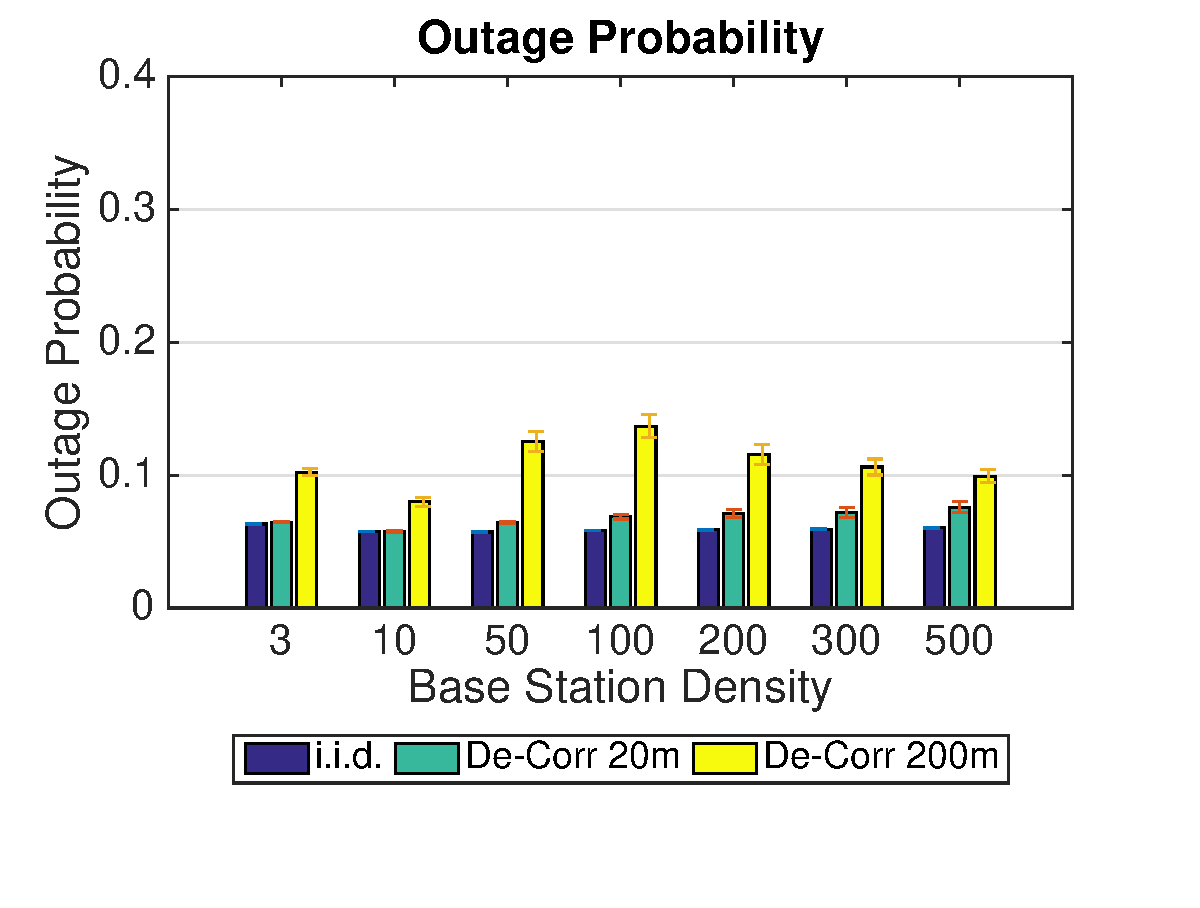
\includegraphics[width=10cm]{MaxMax1000OutageProbThresh-5iid.eps}
 \caption{Outage probability given SINR threshold to be $-5dB$}
 \label{fig: outprobs2}
 \end{figure}
 \begin{figure}
 \centering
 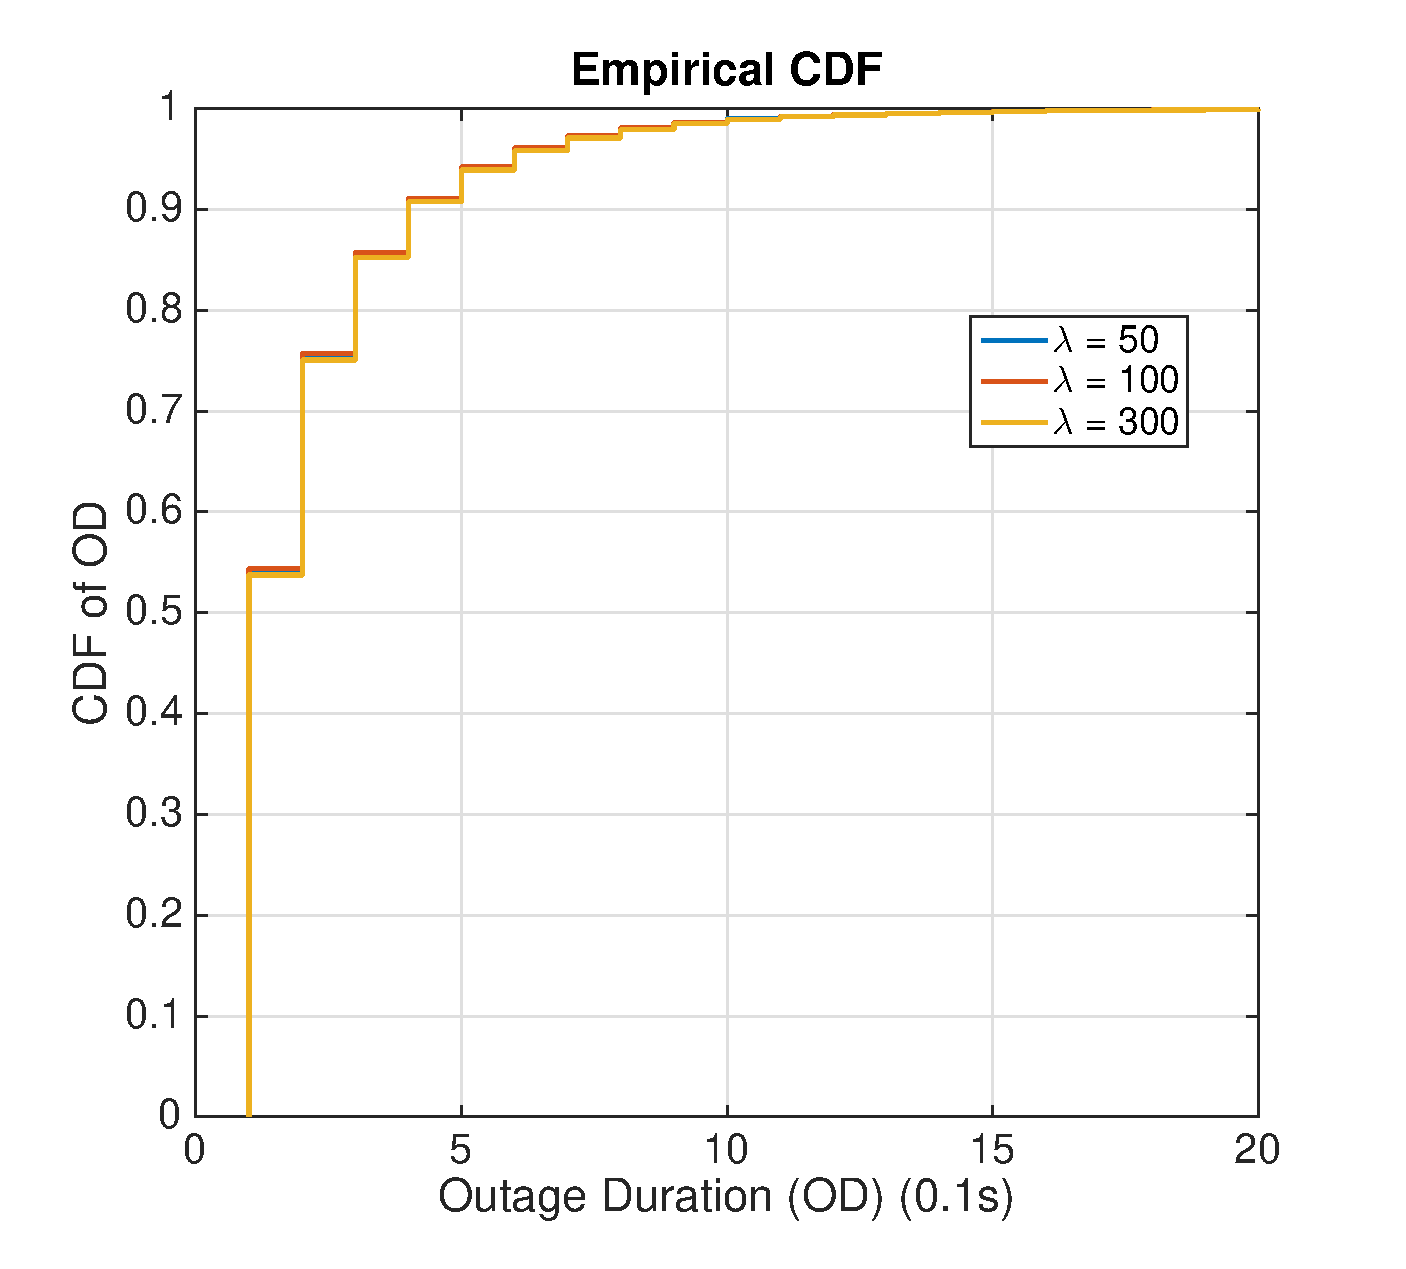
\includegraphics[width=10cm]{ODthresh-5iidNB.eps}
 \caption{CDF of Outage Duration of MU when connecting to the Nearest BS with i.i.d. shadowing}
 \label{iid1}
 \end{figure}
 \begin{figure}
 \centering
 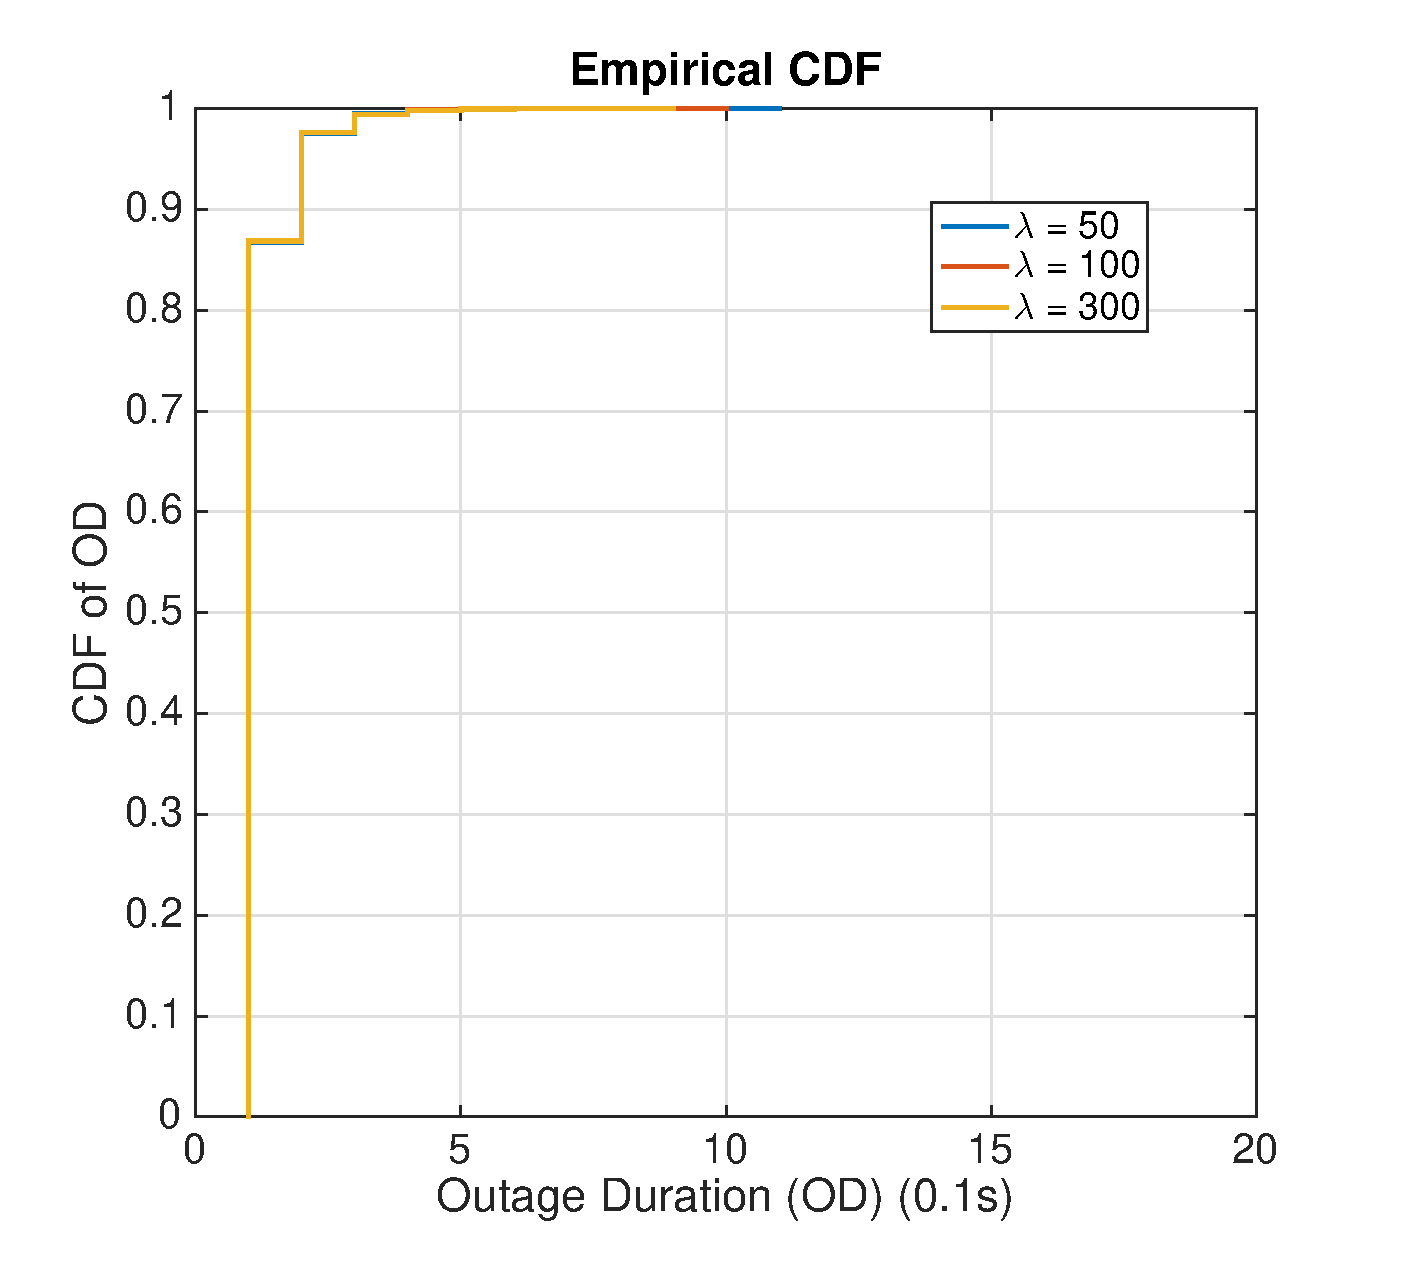
\includegraphics[width=10cm]{ODthresh-5iidMax.eps}
 \caption{CDF of Outage Duration of MU when connecting to the Strongest BS with i.i.d. shadowing}
 \label{iid2}
 \end{figure}
 \begin{figure}
 \centering
 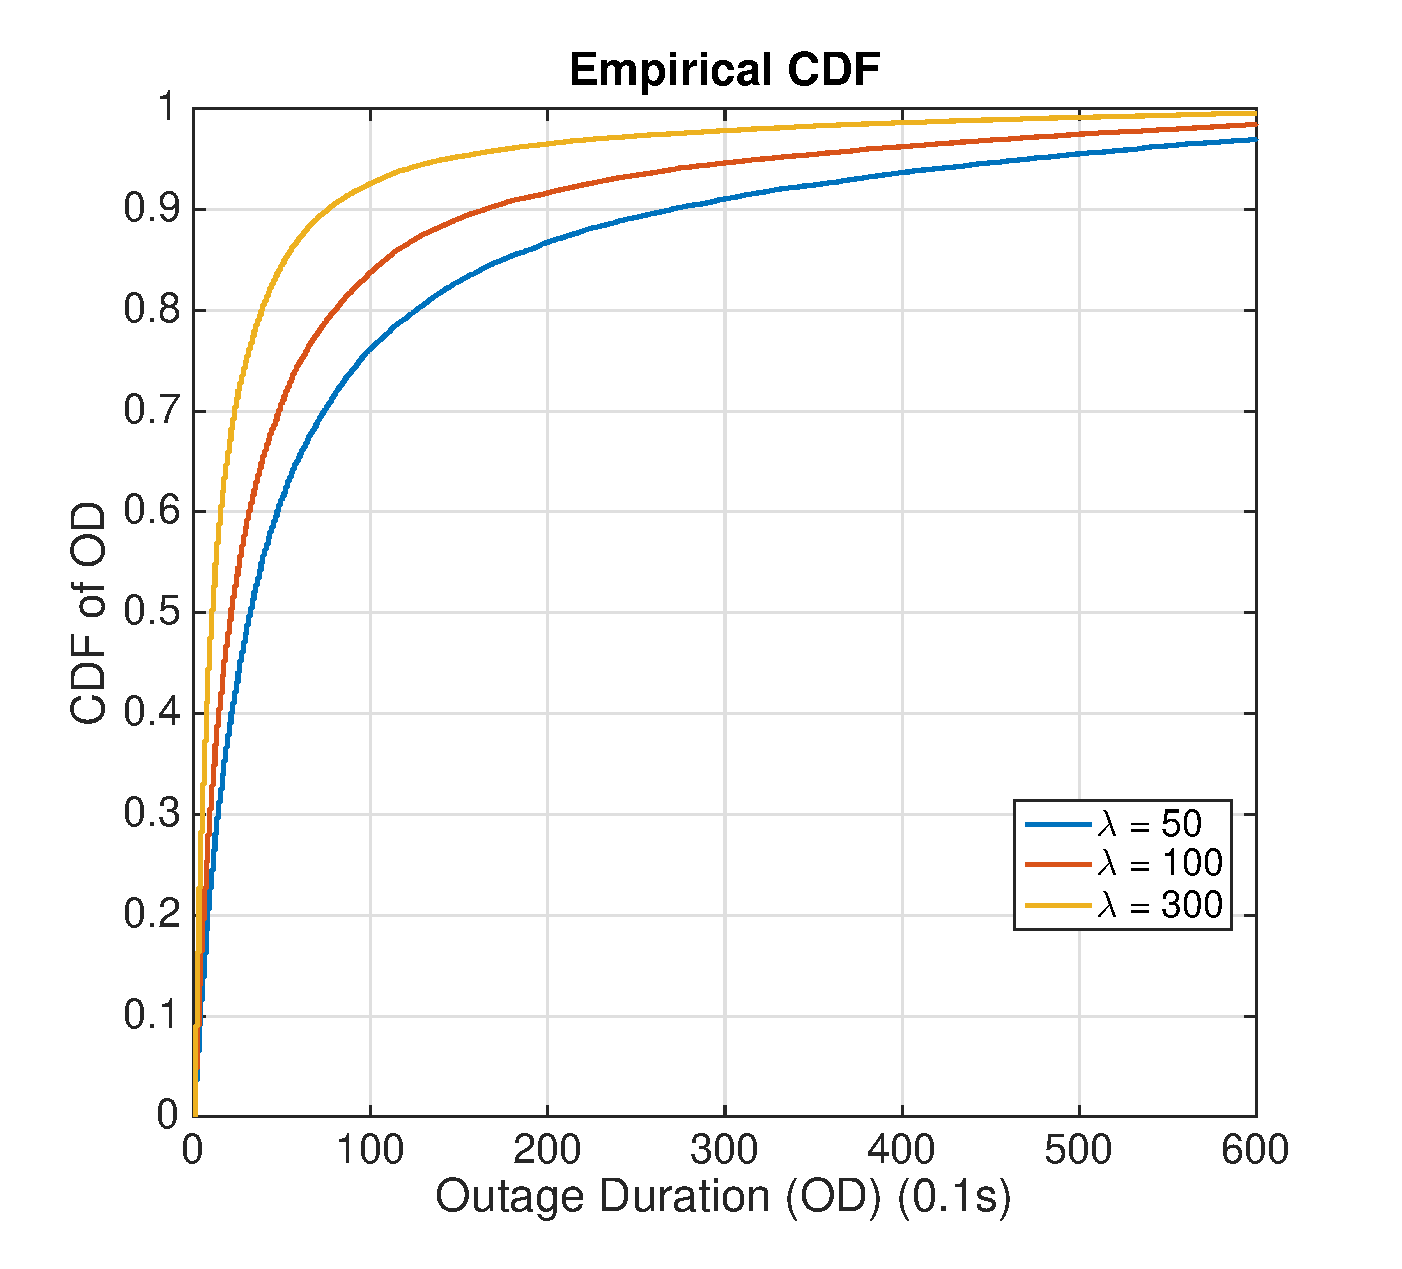
\includegraphics[width=10cm]{ODthresh-5DeCorr200NB.eps}
 \caption{CDF of Outage Duration of MU when connecting to the Nearest BS with correlated shadowing (De-Correlation distance: 200m)}
 \label{corr1}
 \end{figure}
 \begin{figure}
 \centering
 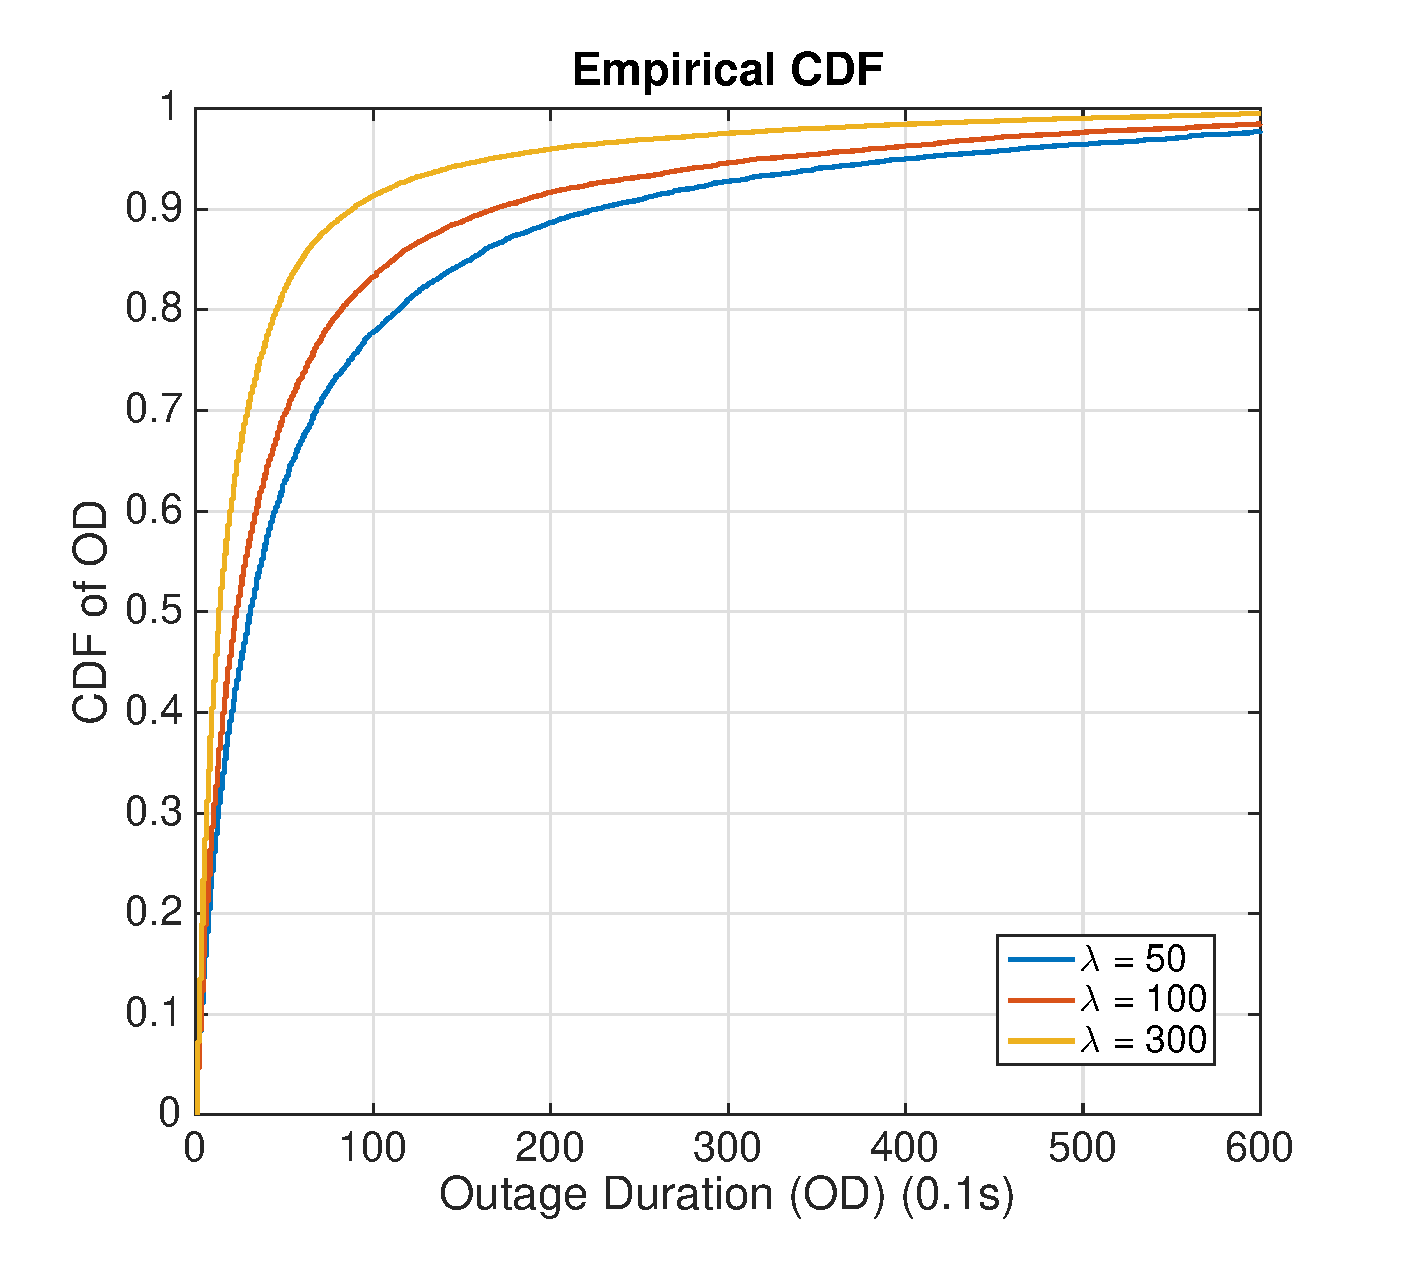
\includegraphics[width=10cm]{ODthresh-5DeCorr200Max.eps}
 \caption{CDF of Outage Duration of MU when connecting to the Strongest BS with correlated shadowing (De-Correlation distance: 200m)}
 \label{corr2}
 \end{figure}
 \par Next we move forward to investigate the system performance when the MU chooses to connect to the BS which provides the highest SINR. Same simulations as the nearest BS scenario are executed to explore this scenario. Figure \ref{4:Mode12}, \ref{4:Mode22} and \ref{4:Mode32} present the SINR of MU when connecting to the strongest BS. From Figure \ref{4:Mode12}, \ref{4:Mode22} and \ref{4:Mode32} we can see that CDF curves of SINR almost overlap each other when increasing BS densities, which means increasing BS density will not change CDF of SINR significantly. Figure \ref{fig: outprobs2} shows outage probability result which is consistent with our conclusion. For each shadow fading model, the difference between highest outage probability and lowest outage probability is less than $5\%$. Comparing three different shadow fading models, we can conclude that when the MU is connecting to the strongest BS, long de-correlation distance will harm the system performance in terms of outage probability (yellow bars are higher than green or blue bars). 
 \par Comparing Figure \ref{fig: outprob1} and Figure \ref{fig: outprobs2}, we find that with same BS density, the outage probabilities are lower for every shadow fading model if MU is connecting to the strongest BS. For example, with independent shadow fading and BS density to be $50$, the outage probability of Nearest BS mode is $38\%$ while that of Strongest BS mode is $6\%$. For correlated shadow fading with de-correlation distance being $200m$ and the BS density being $50$, we find that the outage probability of Nearest BS mode is around $30\%$. This is higher than that of the Strongest BS mode, which is $14\%$. Therefore,we conclude that connecting to the BS which provides highest SINR will improve the system performance with regard to the same network setup. 








 \par In the end, we investigate the system performance form the prospect of outage duration. We use Random Waypoint mobility model to model the user mobility. The parameters of the Random WayPoint model is given in Table \ref{RWP}. The MU speed is assumed to be between $1m/s$ (pedestrian speed) and $20m/s$ (car speed). The MU pause interval is assumed to be uniformly distributed between $0s$ to $60s$. The simulation time is set to be $0.1s$, which means for every $0.1s$ we check the MU's SINR to determine if it is in the outage area or not. Simulation results are shown in Figure \ref{iid1}, \ref{corr1}, \ref{iid2} and \ref{corr2}. Comparing Figure \ref{iid1} and Figure \ref{corr1}, Figure \ref{iid2} and Figure \ref{corr2}, we can see that when the channel is experiencing independent shadow fading, the outage duration is usually less than $2s$. However,  when the channel is under correlated shadow fading with de-correlation distance equal to $200m$, the outage duration can be longer than $30s$. Therefore, we draw the conclusion that correlated shadow fading leads to long-lasting outage durations and harm the system performance. Comparing Figure \ref{iid1} and Figure \ref{iid2}, we find that with independent shadow fading, connecting to strongest BS will reduce the outage duration.  Nevertheless, Figure \ref{corr1} and Figure \ref{corr2} suggest that changing connection strategy will not differentiate the outage duration distributions, although connecting to strongest BS will reduce outage probability. Both Figure \ref{corr1} and Figure \ref{corr2} indicate that increasing BS density will reduce the percentage of long-lasting outage duration. For example, in Figure \ref{corr1}, when the BS density increase from $50$ to $300$, the probability of outage duration longer than $10s$ is reduced from $24\%$ to $7\%$. In contrast, for independent shadow fading, increase BS density will not change the distribution of outage duration, which is confirmed by Figure \ref{iid1} and Figure \ref{iid2}. All CDF curves of outage durations are the same with different BS densities. 
 \begin{table}
 \centering
 \caption{\label{RWP}Random Waypoint Mobility Model Parameters}

 \begin{tabular}{|c|c|}

 \hline
 Speed Interval & $1 - 20m/s$\\
 \hline
 Pause Interval & $0 - 60s$\\
 \hline
 Simulation Time & $0.1s$\\
 \hline
 \end{tabular}

 \end{table}

 \section{Chapter Summary}
 \label{4:Conclusion}
 Shadow fading is large-scale fading which can cause significant received power loss for a wide area. In general, shadow fading is considered to be independent log-normal to simplify the analysis. However, this is not the real case. In reality, shadow fading at two different positions are correlated to each other. Correlated shadow fading will result in correlated outage events and long-lasting outage durations. To investigate a multi-cell system performance given correlated shadow fading, simulations are run to study the outage probability and outage duration distribution. First of all, the probability of two different BS layout: Grid model and Random model are investigated. We find that Grid Layout performs better than Random Layout. Secondly, outage probability given different BS densities and two different connecting strategies: Nearest BS mode and Strongest BS mode, are simulated. We conclude that connecting to strongest BS will reduce the outage probability comparing with nearest BS from simulation results. Increasing BS density will not reduce outage probability when MU is connecting to the strongest BS. However, when MU is connecting to the nearest BS and the de-correlation distance of correlated shadow fading is large enough, increasing BS density will reduce the outage probability.  At last, we investigate the system performance in terms of outage duration. Simulation results show that correlated shadow fading will result in long-lasting outage durations. Increasing BS density will efficiently reduce the percentage of long-lasting outage durations. Therefore, we suggest dense BS layout might be a proper strategy for next generation mmWave communication networks with correlated shadow fading.
 


\chapter{Transport Layer Protocols for Next Generation Networks}\label{ch:5} 


\par The rapid increase of smartphone usage generates a dramatic increase in demand for capacity in mobile broadband communications every year. The wireless carriers and researchers are therefore exploring the underutilized millimeter wave (mmWave) frequency spectrum for next generation (Fifth Generation) broadband cellular communication networks. A mmWave communication system will provide high speed, high capacity wireless communication networks to users. However, the mmWave channel is sensitive to obstructions, which results in frequent capacity fluctuations. The Transmission Control Protocol (TCP) might not work properly with the new channel; therefore, we first investigate the performance of current TCP on mmWave channel. Results indicate that the mmWave channel requires a fast congestion detection scheme and an aggressive recovery scheme. Therefore, this chapter focuses on fast congestion detection scheme and presents a new end-to-end TCP congestion detection scheme for mmWave communication networks: Virtual Explicit Congestion Notification (Virtual ECN). Virtual ECN leads to the possibility of the fast reacting congestion control protocol design.
\section{Introduction}
\par  mmWave channels provide a tremendous amount of capacity and relatively low delay, while suffering from high propagation loss and sensitivity to blockage. Simulations and measurements revealed that the capacity gain is significant, compared to current cellular systems \cite{akdeniz2014millimeter,bai2015coverage}. The last hop wireless channel capacity is no longer a bottleneck; however, mmWave channels are prone to variations due to the blockage from walls, trees or even the human body \cite{lu2012modeling, zhao201328, alejos2008measurement}. This feature brings frequent capacity variations to the channel. Typically, the channel switches periodically between Line-of-Sight (LOS) and Non-Line-of-Sight (NLOS). The upper layer channel provided by a mmWave communication network is not yet standardized. But in general, there is a consensus that mmWave channel will provide high capacity and low latency with frequent capacity fluctuations. For mmWave wireless communication networks, the legacy TCP congestion control might not work well due to its slow congestion detection and conservative loss recovery. Our investigation of TCP over an emulated mmWave channel confirms this. Therefore, designing a new TCP congestion control scheme without involving any intermediate network device is necessary. In this chapter, we will illustrate the initial step to design such a scheme: an end-to-end data-driven fast congestion detection algorithm.
\par In recent years, several promising TCP congestion control protocols have been developed such as BIC TCP \cite{xu2004binary}, CUBIC TCP \cite{ha2008cubic}, and Compound TCP \cite{tan2006compound}. Most of these TCP congestion control schemes rely on three duplicate ACKs or Retransmission Timeout to detect congestion and packet loss. This means TCP needs to wait for at least three ACKs or a retransmission timeout before entering into the recovery mode or the slow start mode. Slow congestion detection reduce the network performance for a high capacity, low latency mmWave channel with frequent capacity variations. First, more congestion and packet loss might occur during this interval and cause high cost to recover from the loss for a high capacity link. Secondly, for a network with capacity variations, the slow congestion detection scheme might provide out of date information on the congestion status, which makes the TCP congestion control protocol extremely conservative.
\par This chapter is organized as follows: Section \ref{Related Work and Motivations} explains the related work on TCP congestion control and mmWave channel. The motivation to design a new scheme is presented in this section. In section \ref{legacy}, we investigate the legacy TCP congestion control performance on an emulated mmWave channel for both NewReno and Cubic. Section \ref{Design} demonstrates the proposed fast end-to-end congestion detection scheme in detail, including network simulation setup, data process and congestion prediction. Section \ref{Conclusions and Future Work} summarizes the chapter and proposes future work, which can be accomplished based on this scheme.

\section{Related Work}
\label{Related Work and Motivations}
In this section, we present the related work on mmWave channel modeling and data-driven TCP congestion control.  
\subsection{mmWave Channel}
\par In \cite{niu2015survey}\cite{rappaport2013millimeter}, research on the feasibility of using mmWave to provide wireless communication service is presented. In \cite{akdeniz2014millimeter}, researchers investigated the mmWave propagation loss, penetration loss, and interference and provided a detailed statistical mmWave channel model based on outdoor measurement. This model elaborated that a mmWave system can provide an order of magnitude increase in capacity. In addition, the probabilities of outage and non-outage were demonstrated. Coverage design technology and beam-forming scheme were discussed in\cite{sun2014millimeter} \cite{roh2014millimeter}, which gives a convincing case for mmWave as the basis for future wireless communication network design. Although the mmWave channel can provide high capacity and low latency, it has one disadvantage: mmWave is sensitive to obstructions like buildings, trees and even nearby pedestrians or vehicles. These obstructions may cause sudden, short and severe channel downgrade. How to increase the reaction speed to the channel fluctuations and fully utilize the channel capacity is the main issue for TCP congestion control protocol design. This chapter focuses on solving this problem from an end-user perspective.
eth
\subsection{Explicit Congestion Notification (ECN)}
\par Legacy TCP congestion control protocols consider duplicate ACKs as an indication of packet loss. With the addition of active queue management and ECN \cite{ramakrishnan2001rfc} to the network infrastructure, routers are capable of detecting congestion before the buffer queue overflows. An additional Congestion Experienced (CE) byte is added to the IP header of the packet to support this function. Routers running RED queue management can mark the CE code point with a certain probability when the average queue length is between the minimal threshold and the maximal threshold. When the average queue length exceeds the maximal threshold, upcoming packets' CE byte will be marked with probability $1$. The packet with marked CE will be sent to the receiver. After receiving the packet, the receiver will piggyback an ACK with marked CE to notify the sender that there is congestion in the router. No extra traffic will be generated to overload the network. The sender will reduce the congestion window to avoid queue overflow and packet loss. Using ECN to detect congestion requires the participation of routers and waiting for the receiver's feedback. We develop an end-user congestion prediction scheme that utilizes the idea of ECN without involving any network devices or waiting for any feedback.
\subsection{Remy}
\par Remy \cite{winstein2013tcp} was proposed by Keith Winstein in 2013. It is a congestion-control scheme based on prior knowledge of the network and the traffic model. It is the first computer generated congestion control protocol. A RemyCC tracks only three state variables of the end-user:
\begin{itemize}
\item An exponentially weighted moving average (EWMA) of the inter-arrival time between new ACKs received (ack\_ewma).
\item An EWMA of the time between TCP sender timestamps reflected in those ACKs (send\_ewma).
\item The ratio between the most recent Round Trip Time (RTT) and the minimum RTT during the current connection (rtt\_ratio).
\end{itemize}
The algorithm does not require support from any intermediate network devices. The end-user can adjust its sending speed following the pre-generated algorithm based on the above mentioned data. This indicates that these three variables together might reflect the congestion state of the network. 


\par Remy is based on the conviction that designing a data-driven congestion detection algorithm using the end-user data is possible. Since ECN provides accurate information of whether there is congestion in the network or not, we decide to use end-user data to predict ECN, thereby detect the congestion. The main contribution of this chapter is developing a data-driven fast congestion detection algorithm (within one ACK inter-arrival time) using the end-user data without support from receivers, routers or any other network devices.

\section{Legacy TCP Performance on Emulated 5G Channel}
\label{legacy}
\par Since Gigabit Ethernet has a similar capacity as a mmWave channel, we use Ethernet with periodic on-off behavior to emulate a mmWave channel. On period means the channel is in the LOS state, while an off period means the channel is in the NLOS state. We test two existing TCP congestion control protocols: NewReno and Cubic, on the emulated mmWave channel. In the GENI Portal \cite{Geni}, a three-node line topology with a server, a middle box and a client is set up as in Figure \ref{genitopo}. 
\begin{figure}
\centering
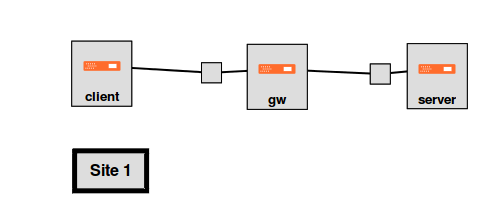
\includegraphics[width=14cm]{topologyGeni.png}
\caption{GENI Topology for Performance Evaluation}
\label{genitopo}
\end{figure}
Two different kinds of channel behavior are investigated: uniformly distributed on-off periods and exponentially distributed on-off periods. Congestion window size (CWND) and throughput are recorded to analyze the performance as in Figures \ref{1st}, \ref{2nd}, \ref{3rd} and \ref{4th}.  The channel capacity is set to be $1$Gbps. Figure \ref{1st} illustrates the CWND of the sender when the off period is exponentially distributed with mean $10ms$, $100ms$, $1s$, while Figure \ref{2nd} shows the corresponding throughput. Figure \ref{3rd} and \ref{4th} presents the CWND and throughput when the off period is uniformly distributed between $0ms - 10ms$, $0ms - 100ms$ and $0ms - 1s$. In both cases, the performance of NewReno deteriorates significantly due to the high frequency of the on-off period. Figures \ref{1st} and \ref{3rd} demonstrate that slow start will be initiated after every off period. The throughput drops to as low as $200$Mbps, which is $20\%$ of the full capacity. Comparing with NewReno, from Figures \ref{1st} and \ref{3rd} we conclude that Cubic is more aggressive than NewReno. When a channel recovers from an off period to an on period, Cubic increases the CWND faster to utilize the channel capacity.  If the channel off time is at the level of 10ms, cubic did not even notice there is a connection drop. Instead, it behaves as if congestion occurred in the network and reduces the CWND. Whenever the on time period is long enough as in the exponentially on-off period case, Cubic can still reach the upper limit of CWND and achieve full throughput as in Figure \ref{2nd}, while NewReno needs more time to recover. In the uniformly distributed on-off period case, the channel lost occurred before Cubic fully recovered as in Figure \ref{3rd}. The CWND has a descending trend and the throughput decreases as time goes on. Based on the aforementioned observation, we conclude that even Cubic will not achieve high throughput if the channel switch between LOS (on) and NLOS (off) with a high frequency. Therefore, an aggressive congestion control protocol is necessary for next generation networks. In the following sections, we will focus on the initial step of design this protocol: developing a fast end-user congestion prediction algorithm.
\begin{figure}
\centering
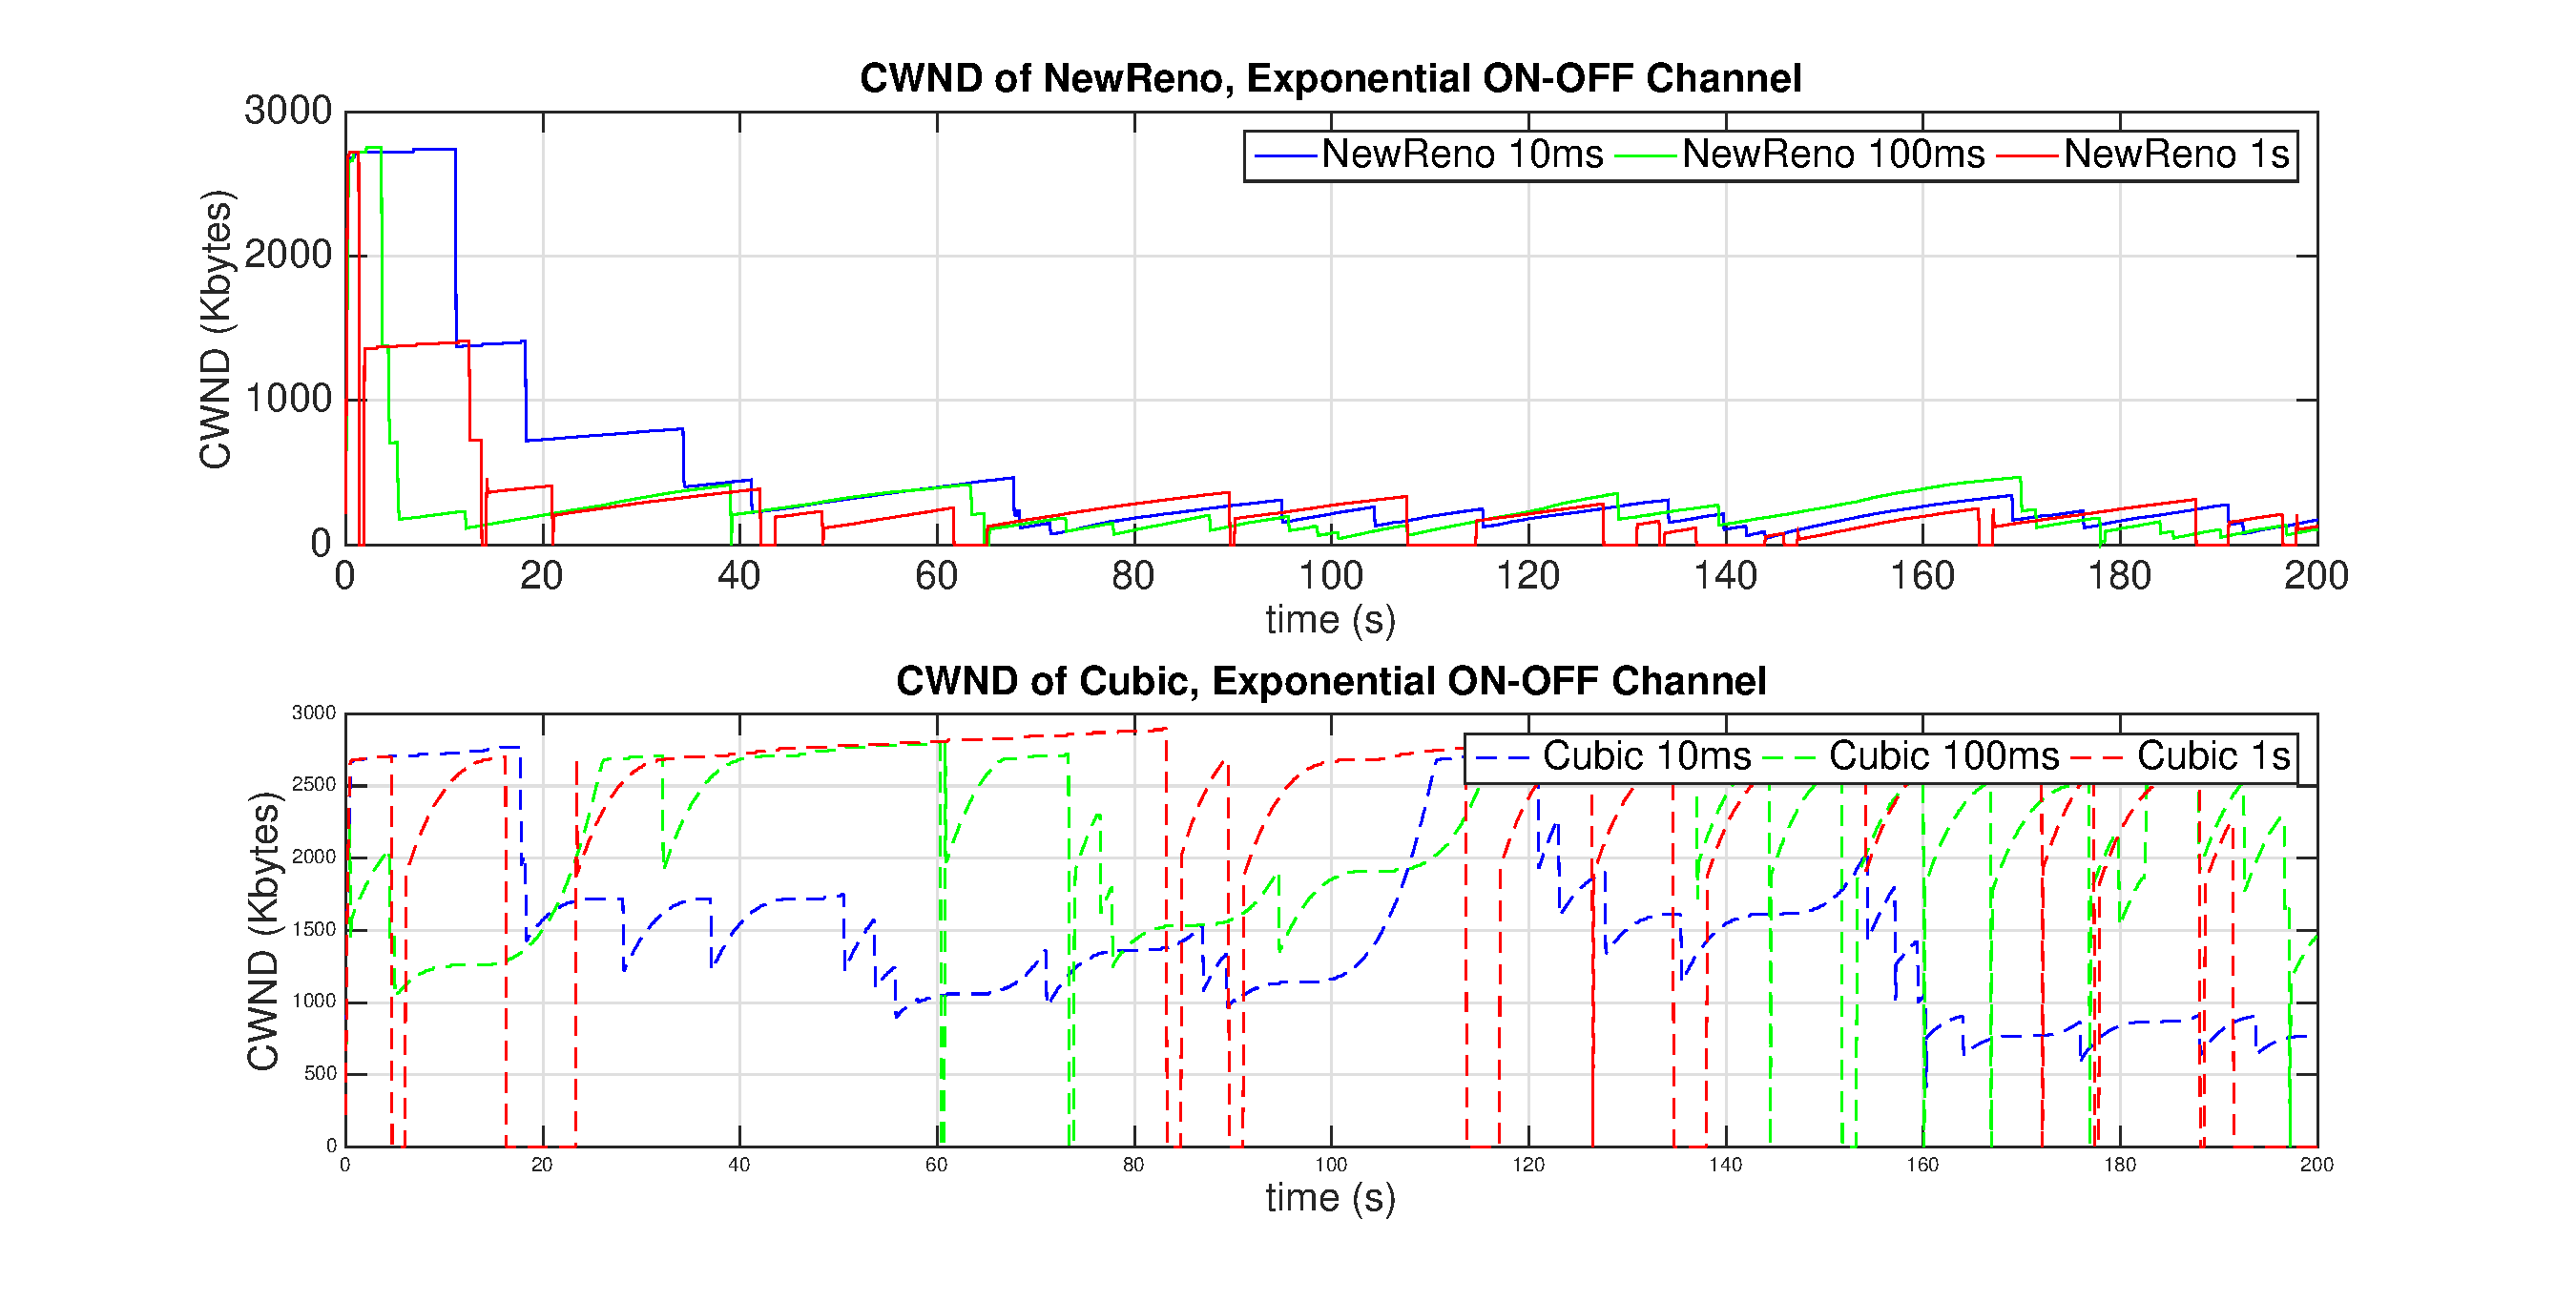
\includegraphics[width=14cm]{1.eps}
\caption{CWND dynamics given exponentially On-Off channel behavior}
\label{1st}
\end{figure}
\begin{figure}
\centering
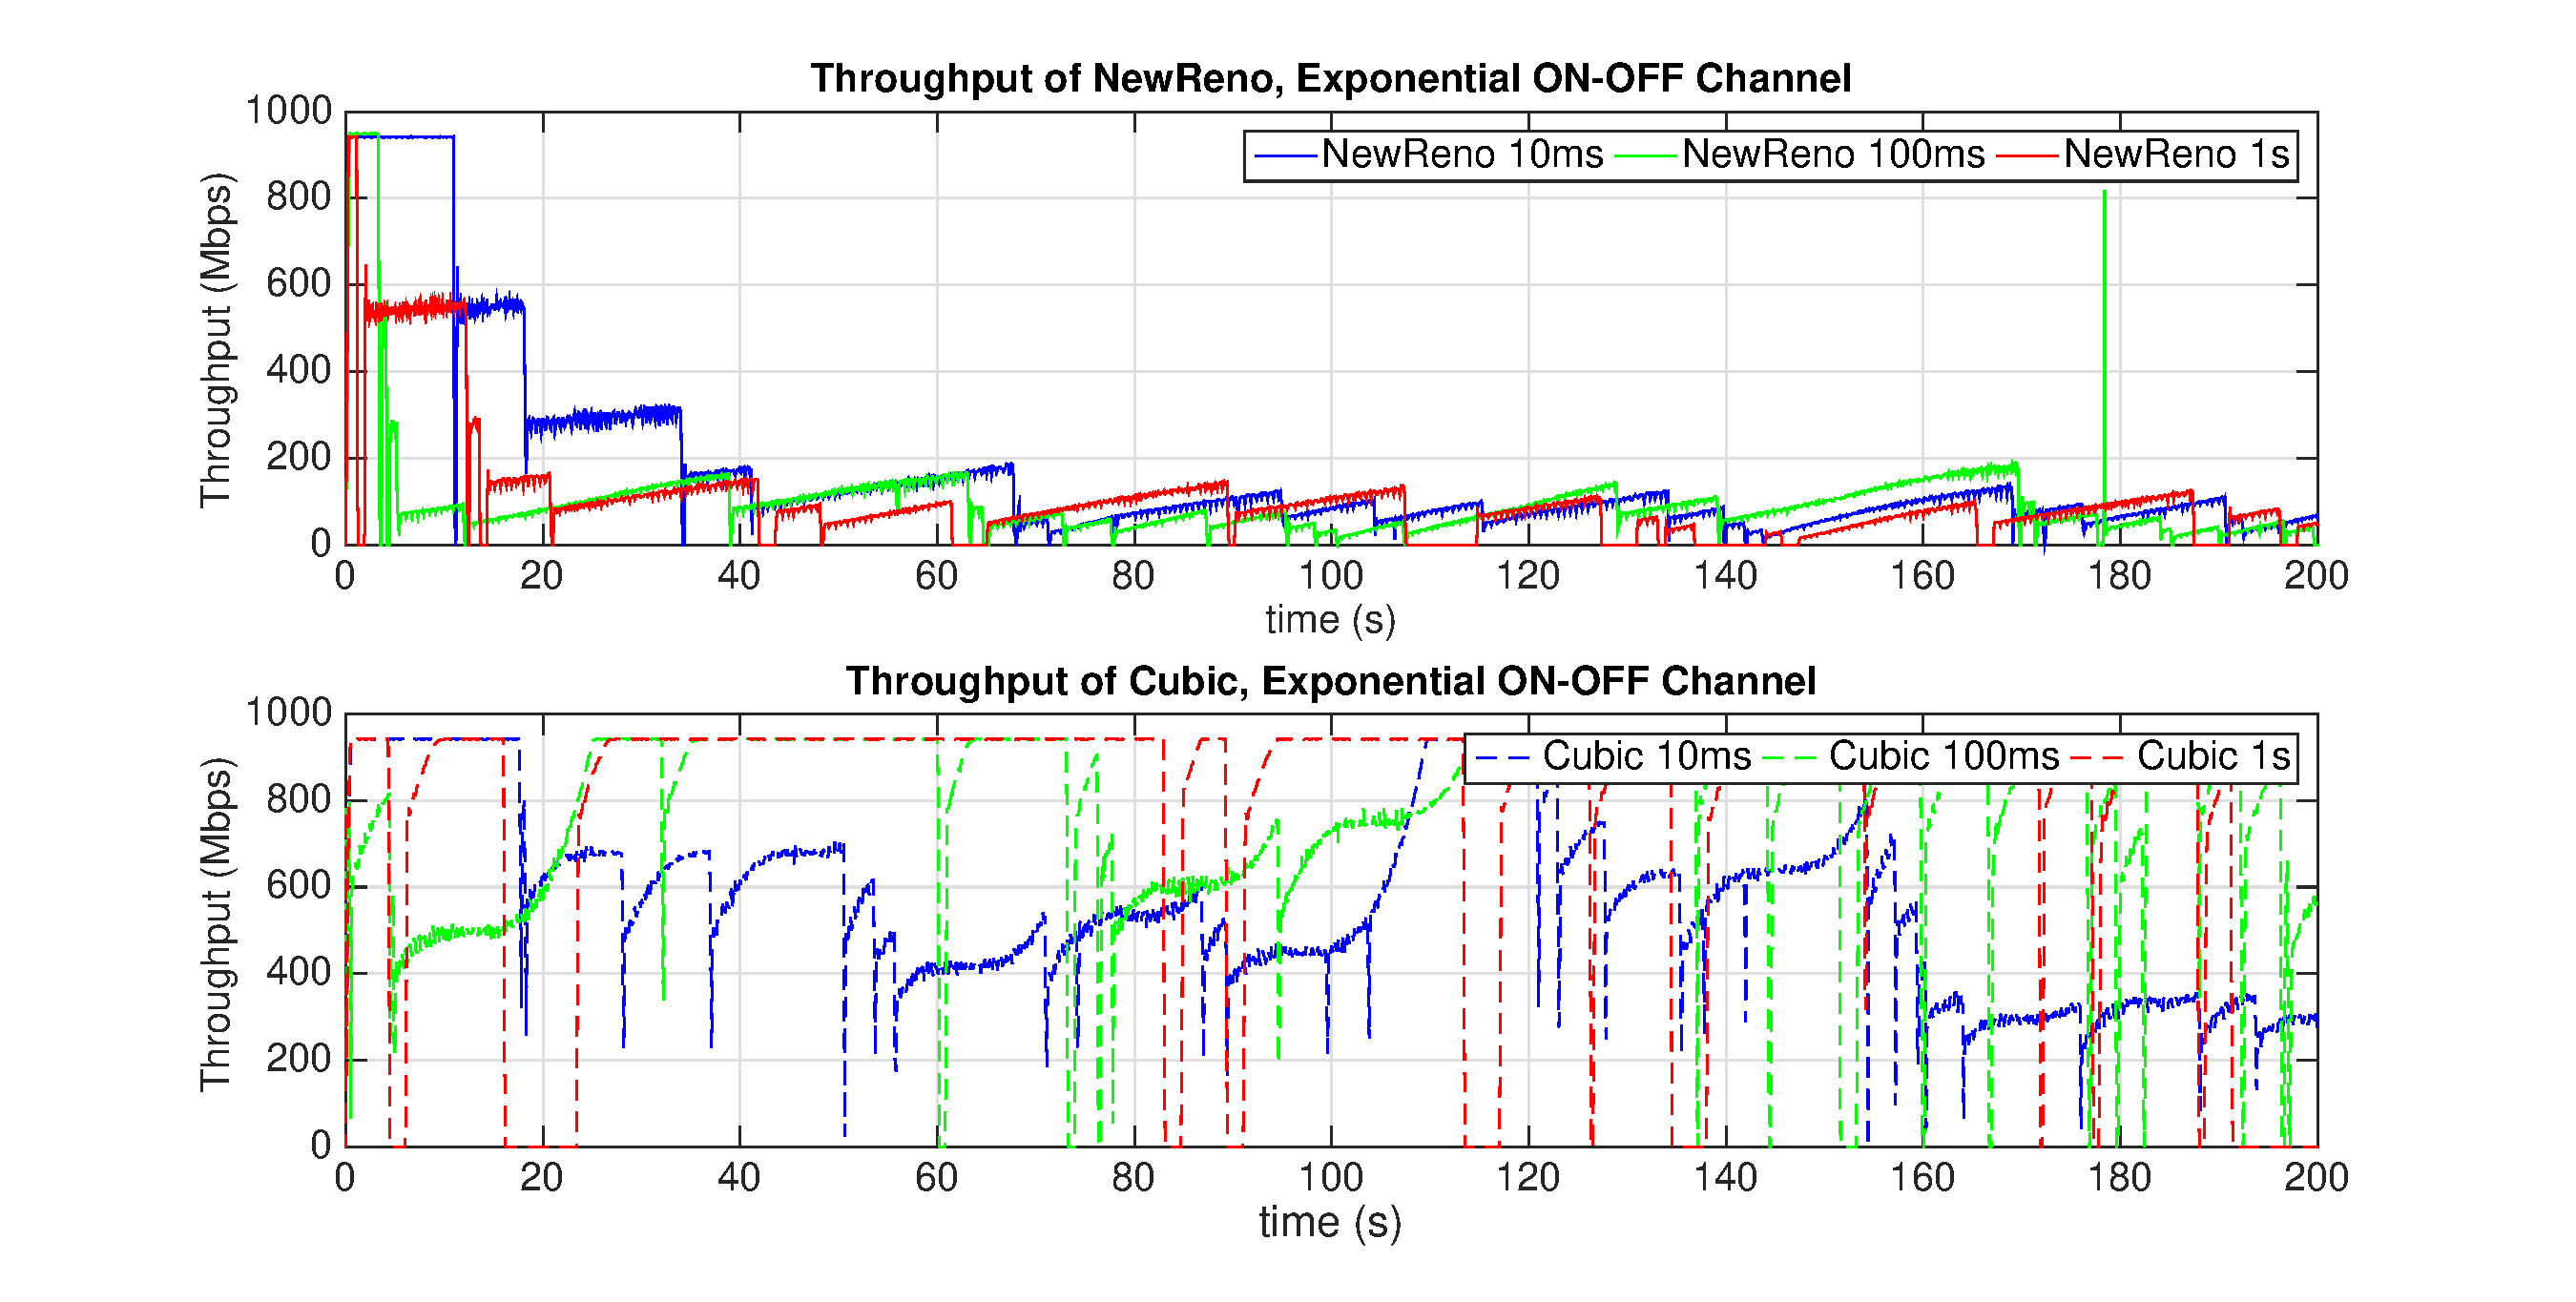
\includegraphics[width=14cm]{2.eps}
\caption{Throughput dynamics given exponentially On-Off channel behavior}
\label{2nd}
\end{figure}
\begin{figure}
\centering
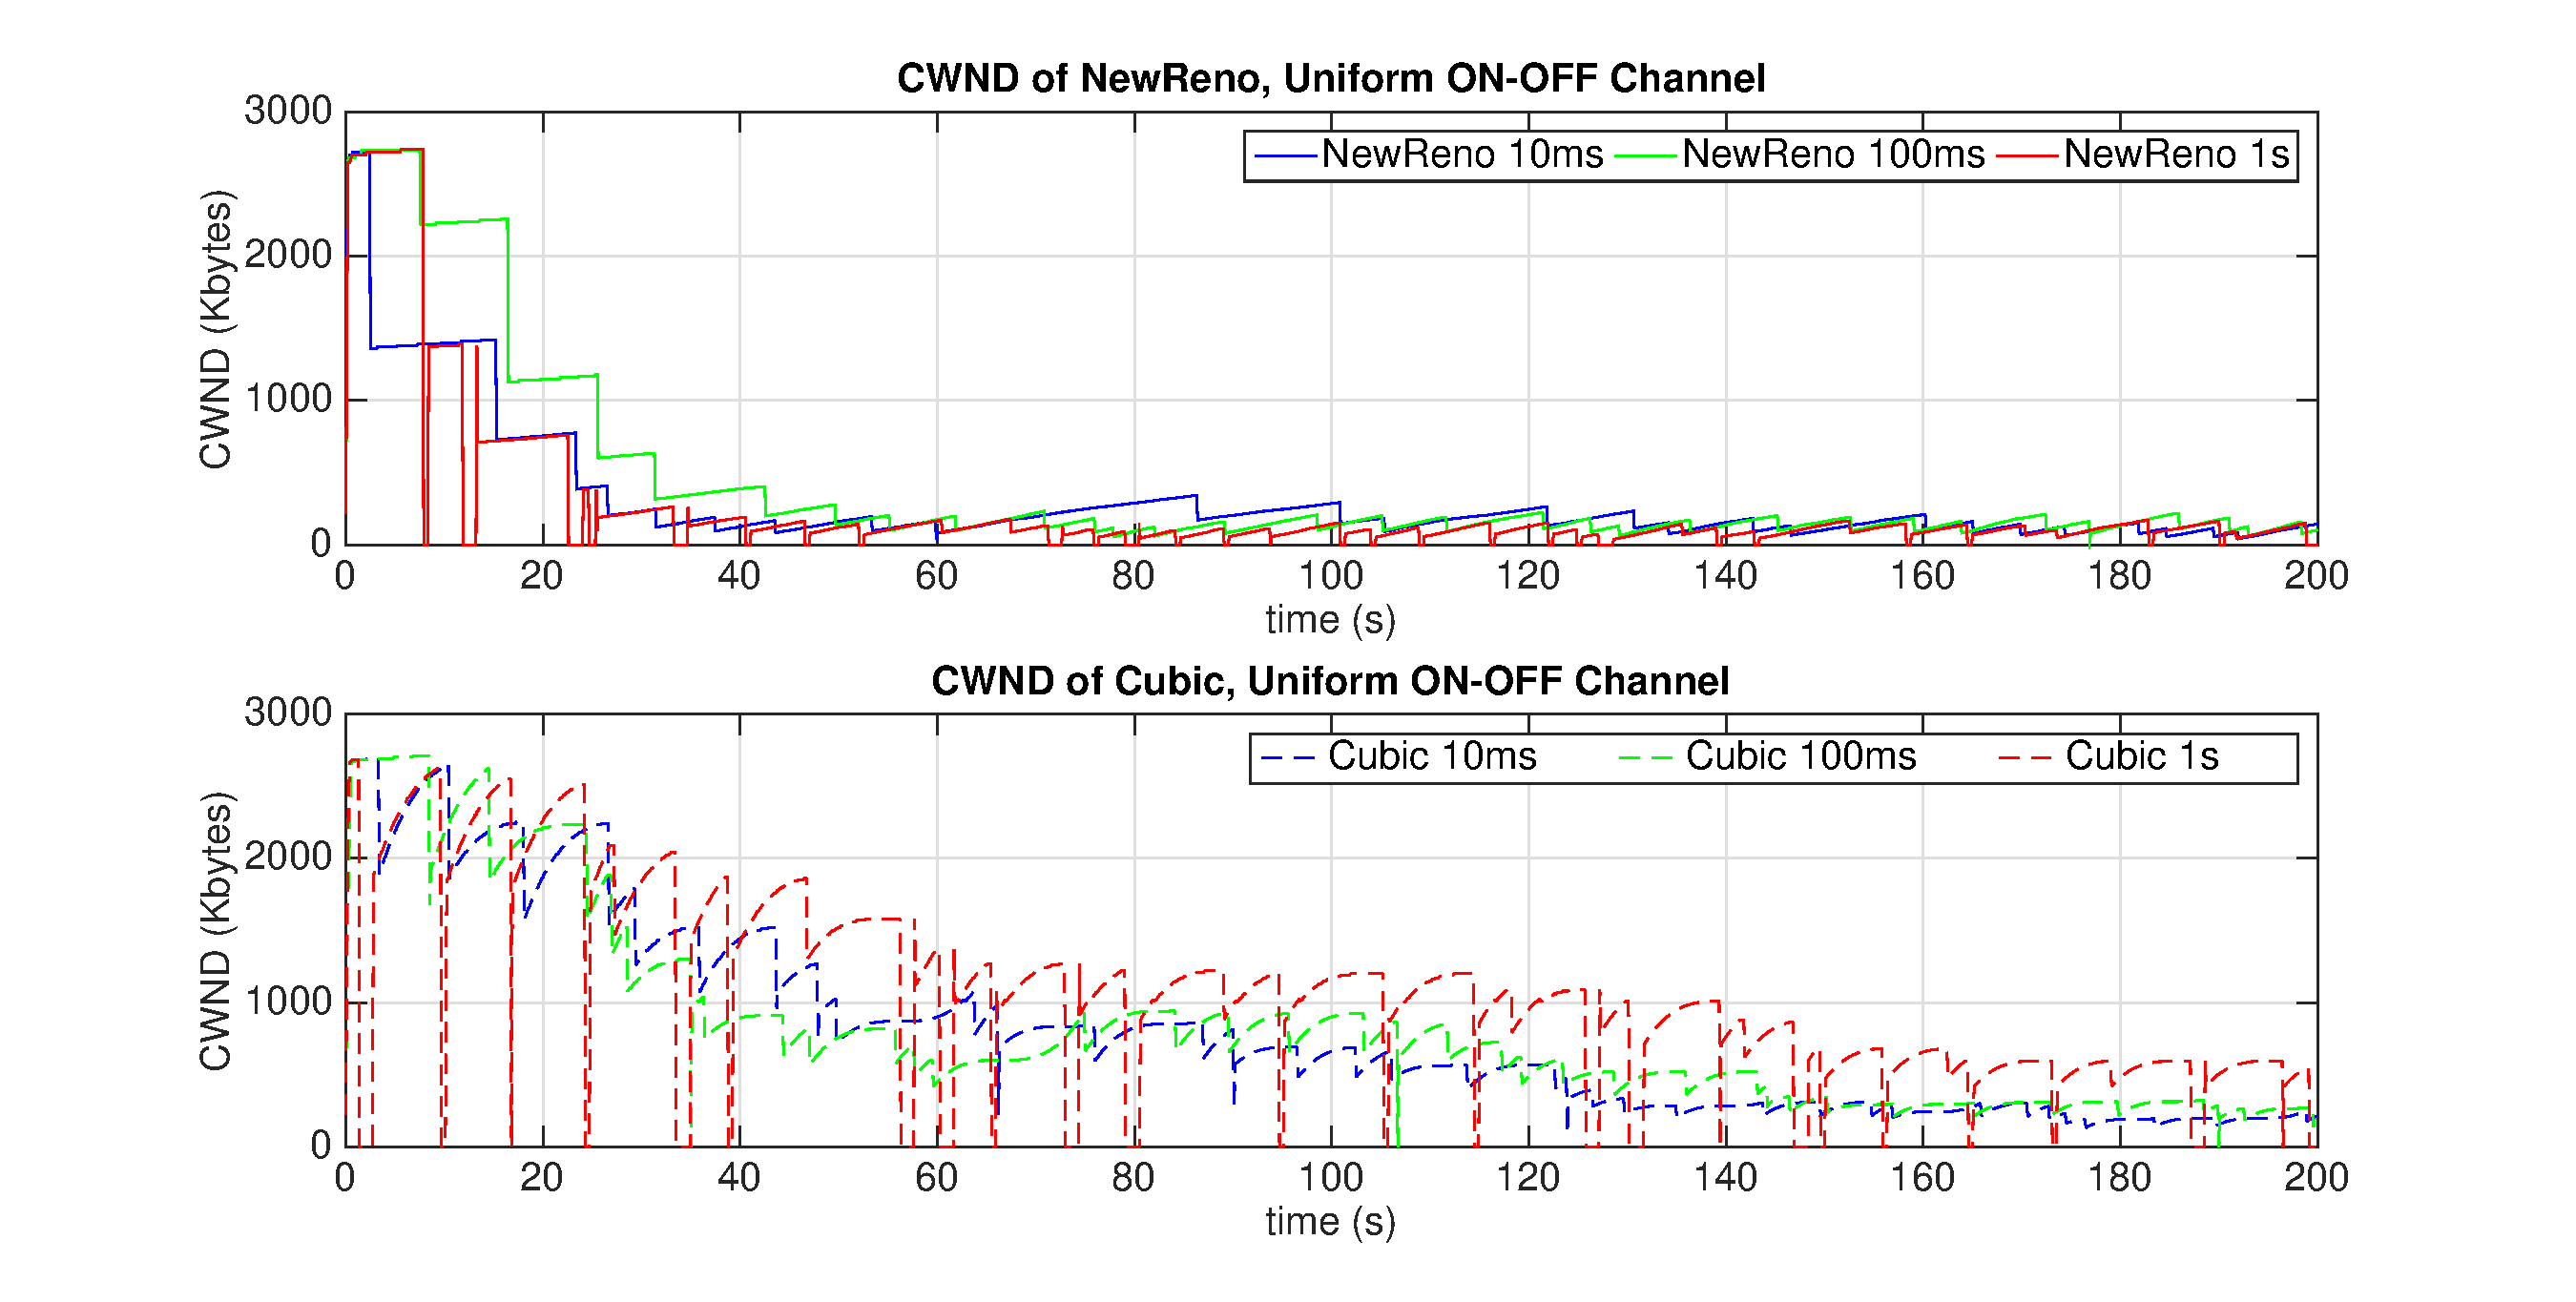
\includegraphics[width=14cm]{3.eps}
\caption{CWND dynamics given uniformly On-Off channel behavior}
\label{3rd}
\end{figure}
\begin{figure}
\centering
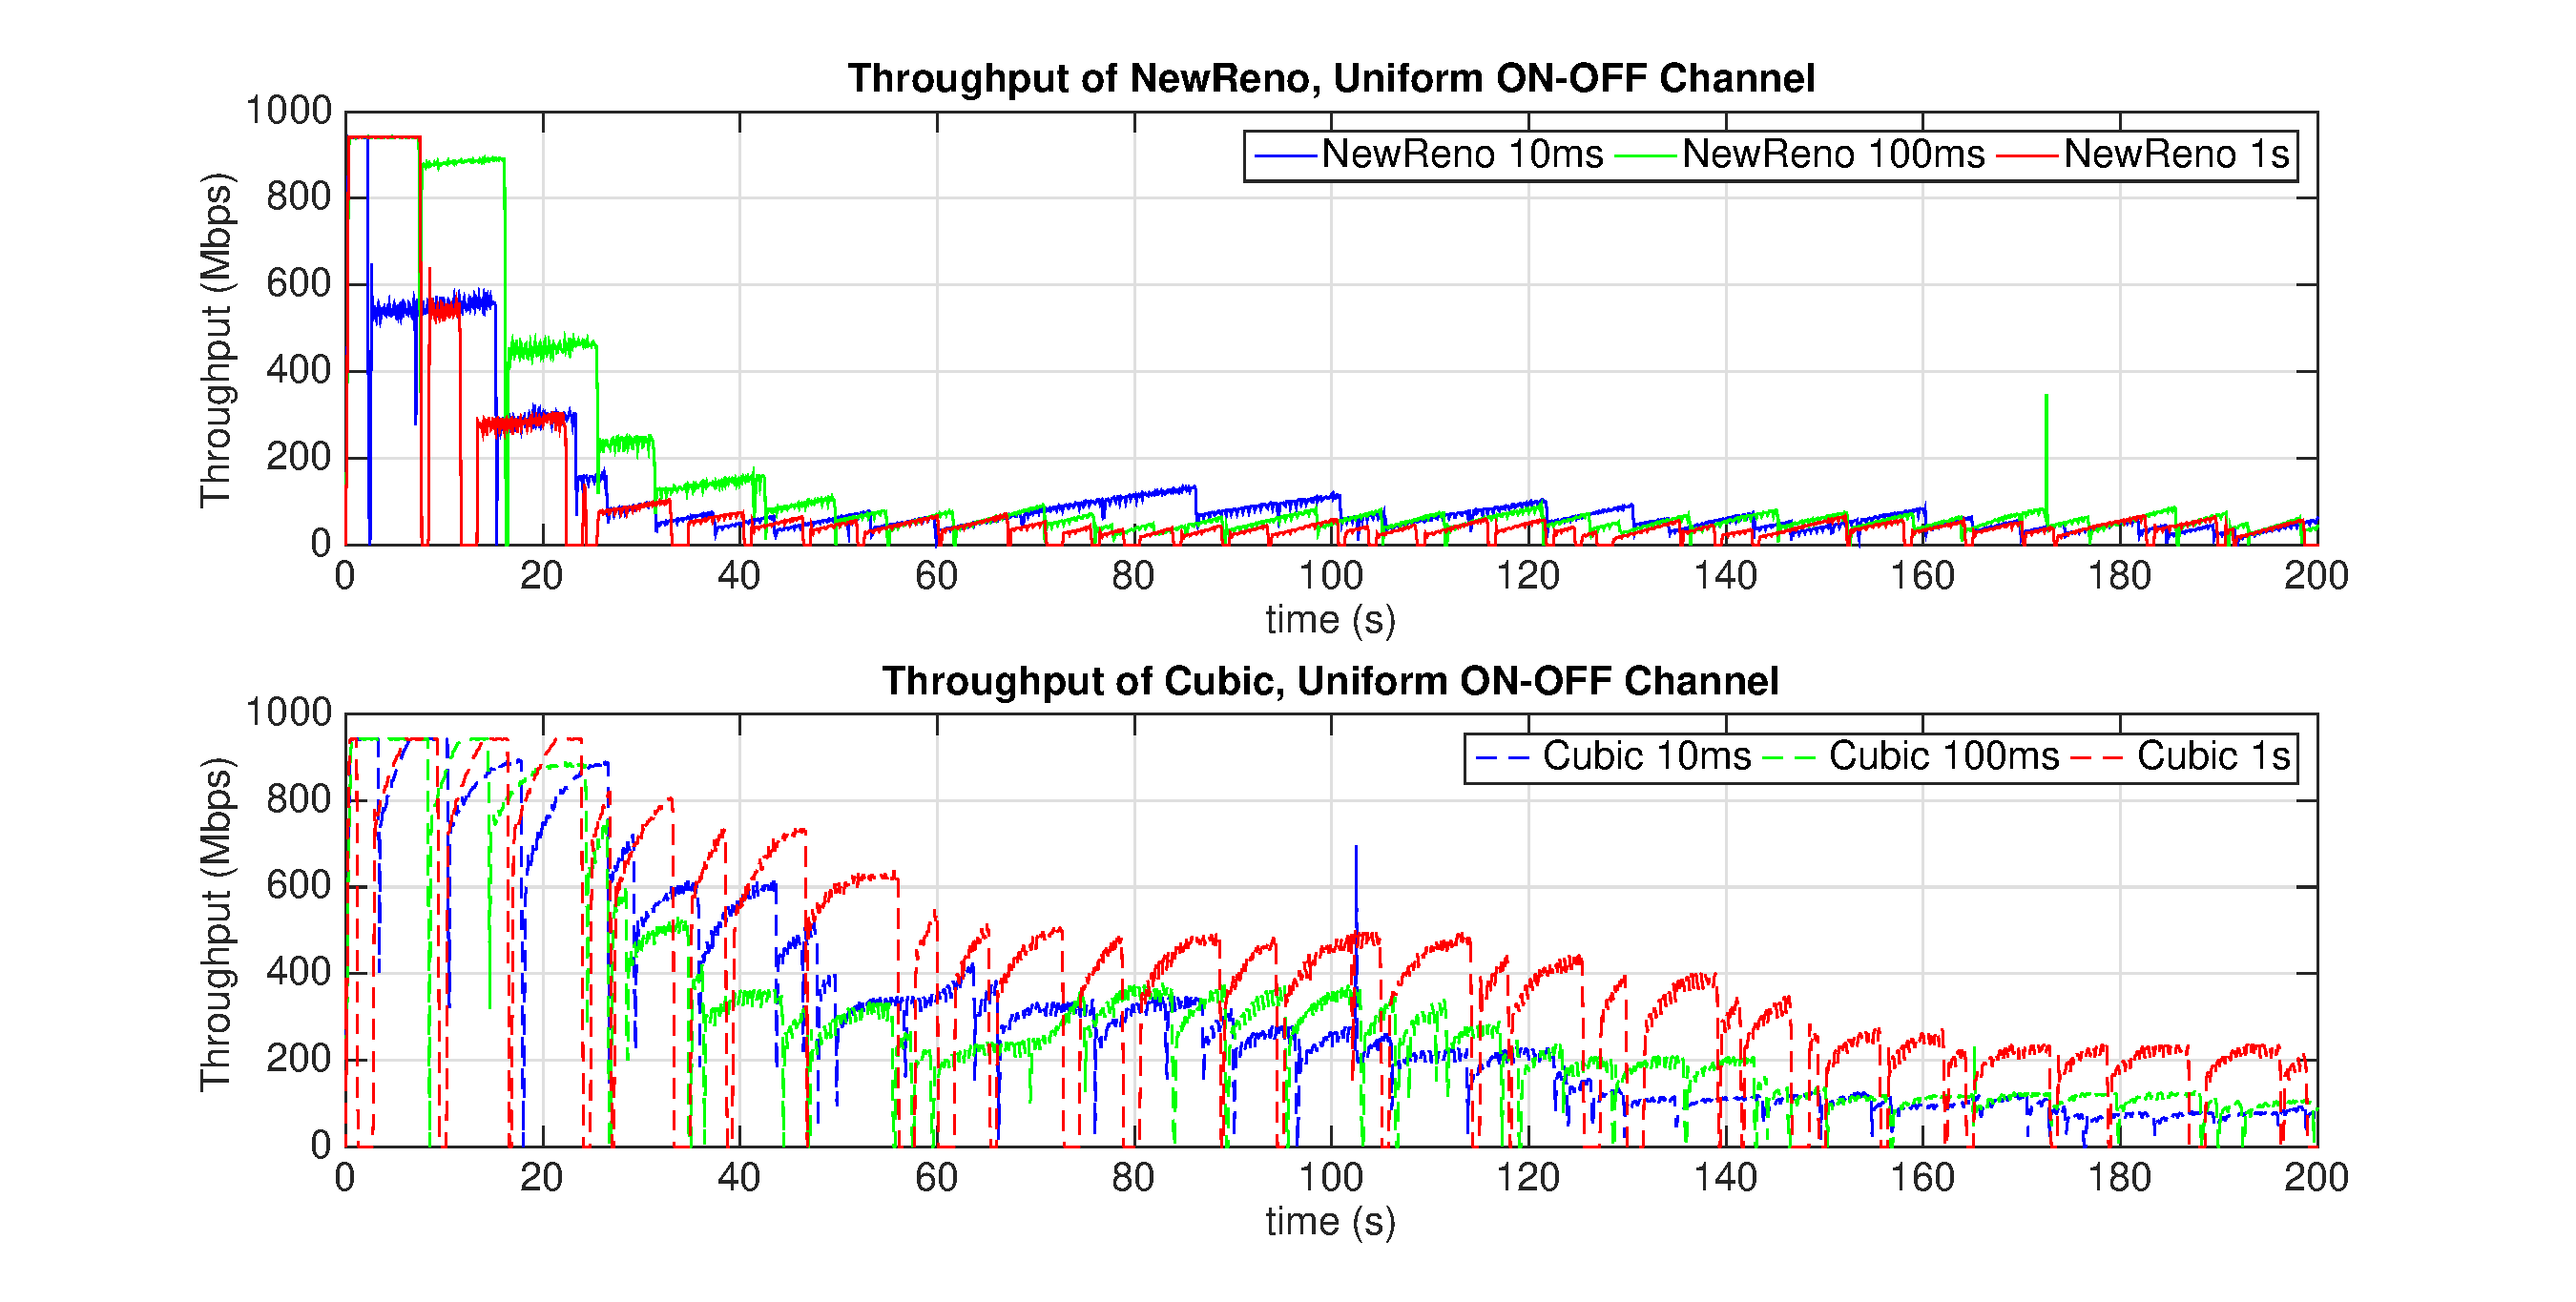
\includegraphics[width=14cm]{4.eps}
\caption{Throughput dynamics given uniformly On-Off channel behavior}
\label{4th}
\end{figure}
\section{Congestion Detection Algorithm}
\label{Design}
The design of the fast congestion detection algorithm is illustrated in detail in this section. The principle idea is to predict the congestion in the network within one inter-arrival time of ACKs using the end-user data. Data which can be collected from the end-user includes packet sending time, ACK arrival time and the RTT calculated from these two timestamps. We run simulations using the discrete event-based Network Simulator 2 (NS2) \cite{NS2} to collect this data for a particular network topology. 
\subsection{Network Topology}
A typical dumbbell model is presented and used in this section. The network topology is shown in Figure \ref{layout}. There are $6$ TCP traffic senders and $6$ receivers; the sender $s_{i}$ sends data to receiver $r_{i}$ through the bottleneck link $Q1\to Q2$. Both $Q1$ and $Q2$ maintain a DropTail Queue. The queue limit is set to be the bandwidth-delay product to ensure the full utilization of the link capacity.
%\begin{figure}[!htb]\centering
%   \begin{subfigure}{0.49\textwidth}
%     \frame{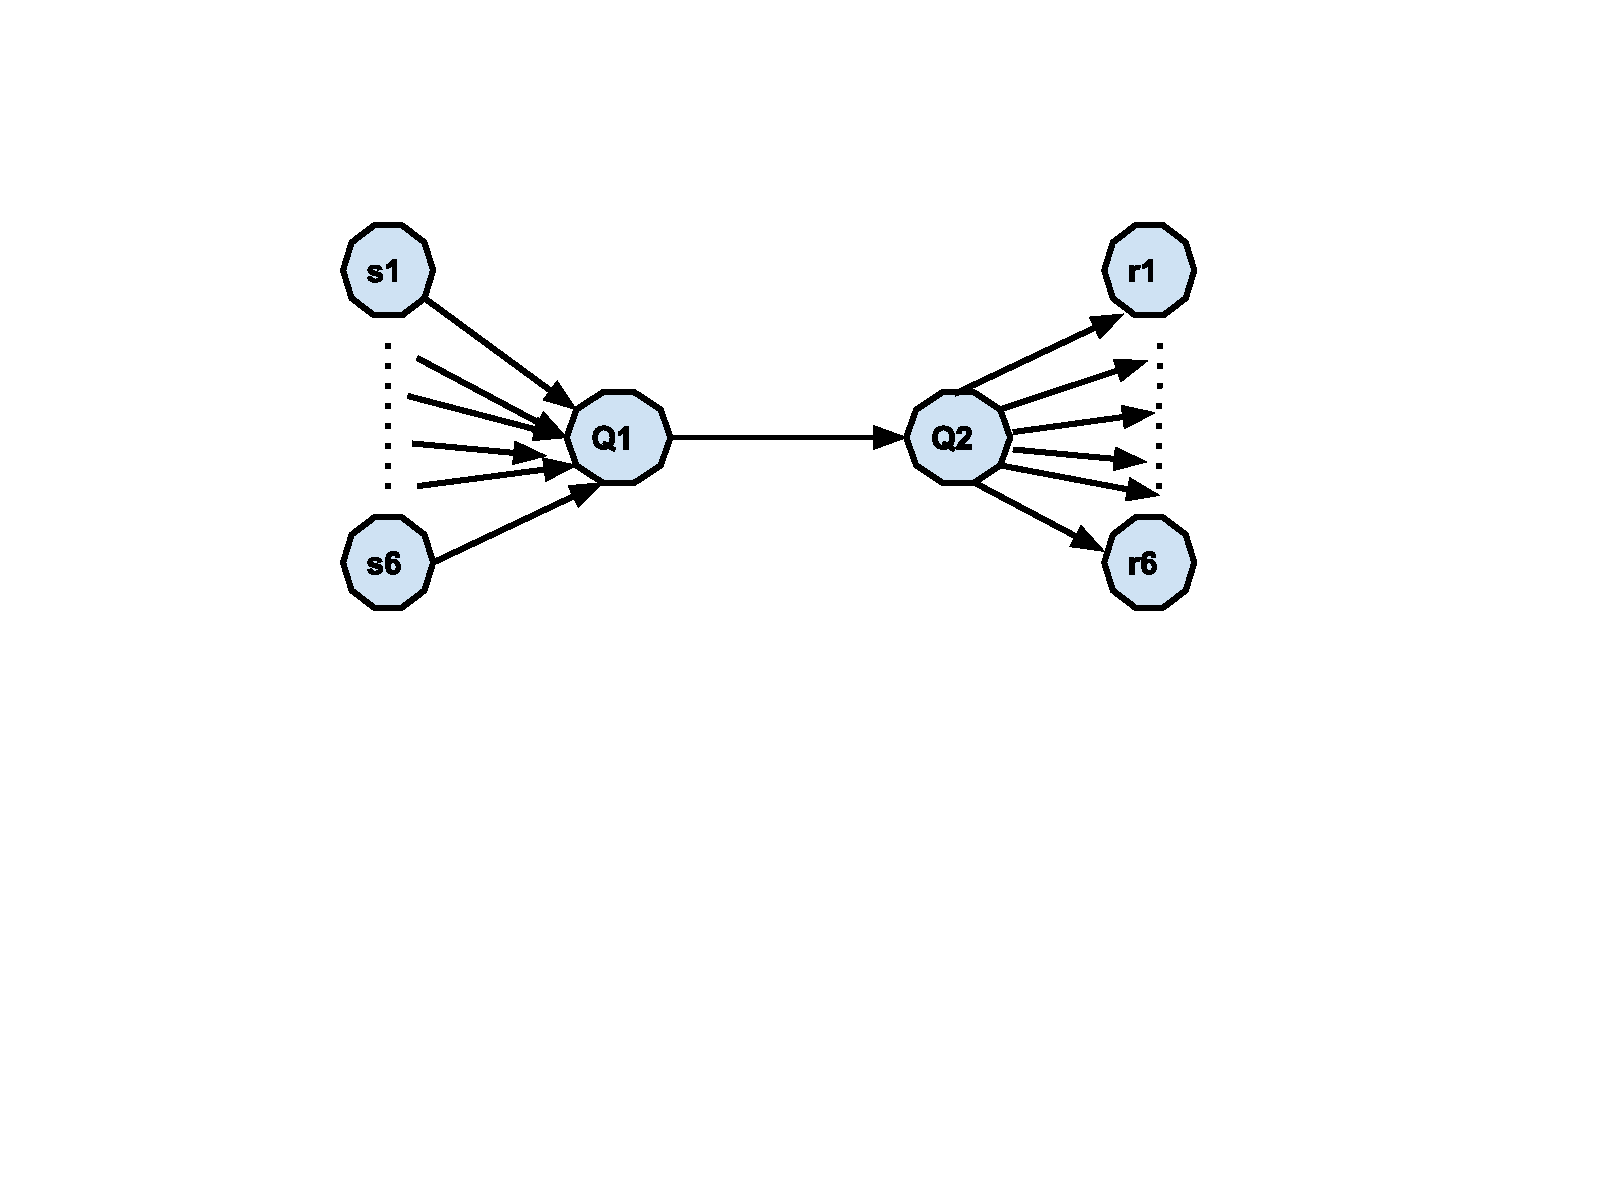
\includegraphics[width=6cm]{6layout.pdf}}
%     \caption{Network Topology}\label{layout}
%   \end{subfigure}
%   \begin {subfigure}{0.49\textwidth}
%     \frame{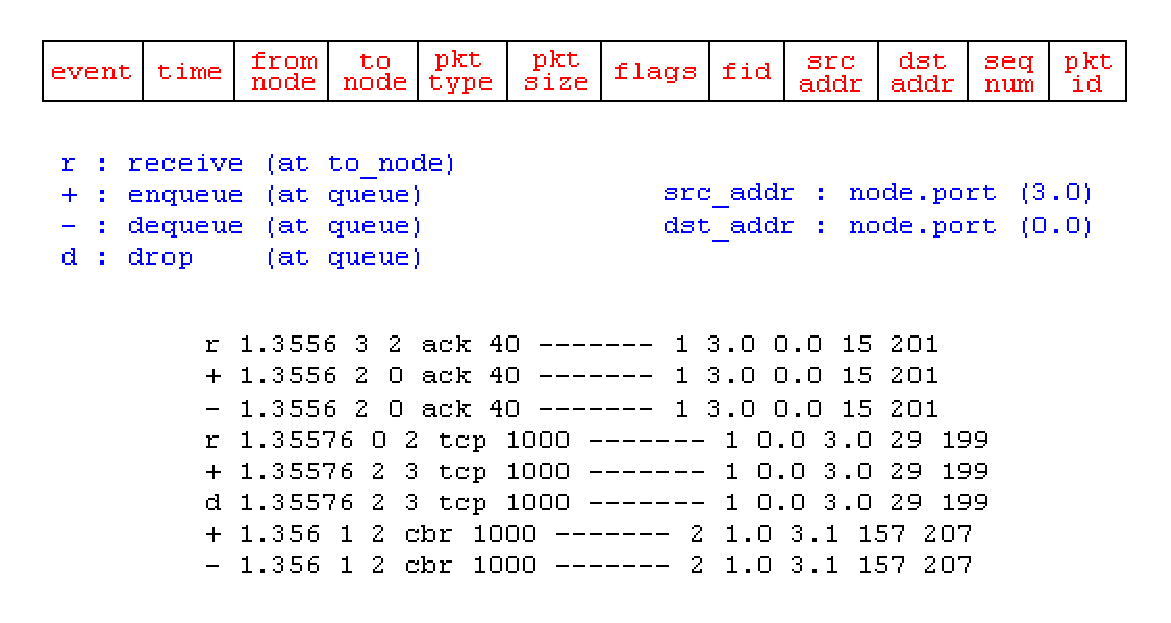
\includegraphics[width=6cm]{format.eps}}
%     \caption{NS2 TCP Trace Format}\label{NS2Format}
%   \end{subfigure}
%\end{figure}

\begin{figure}
\centering
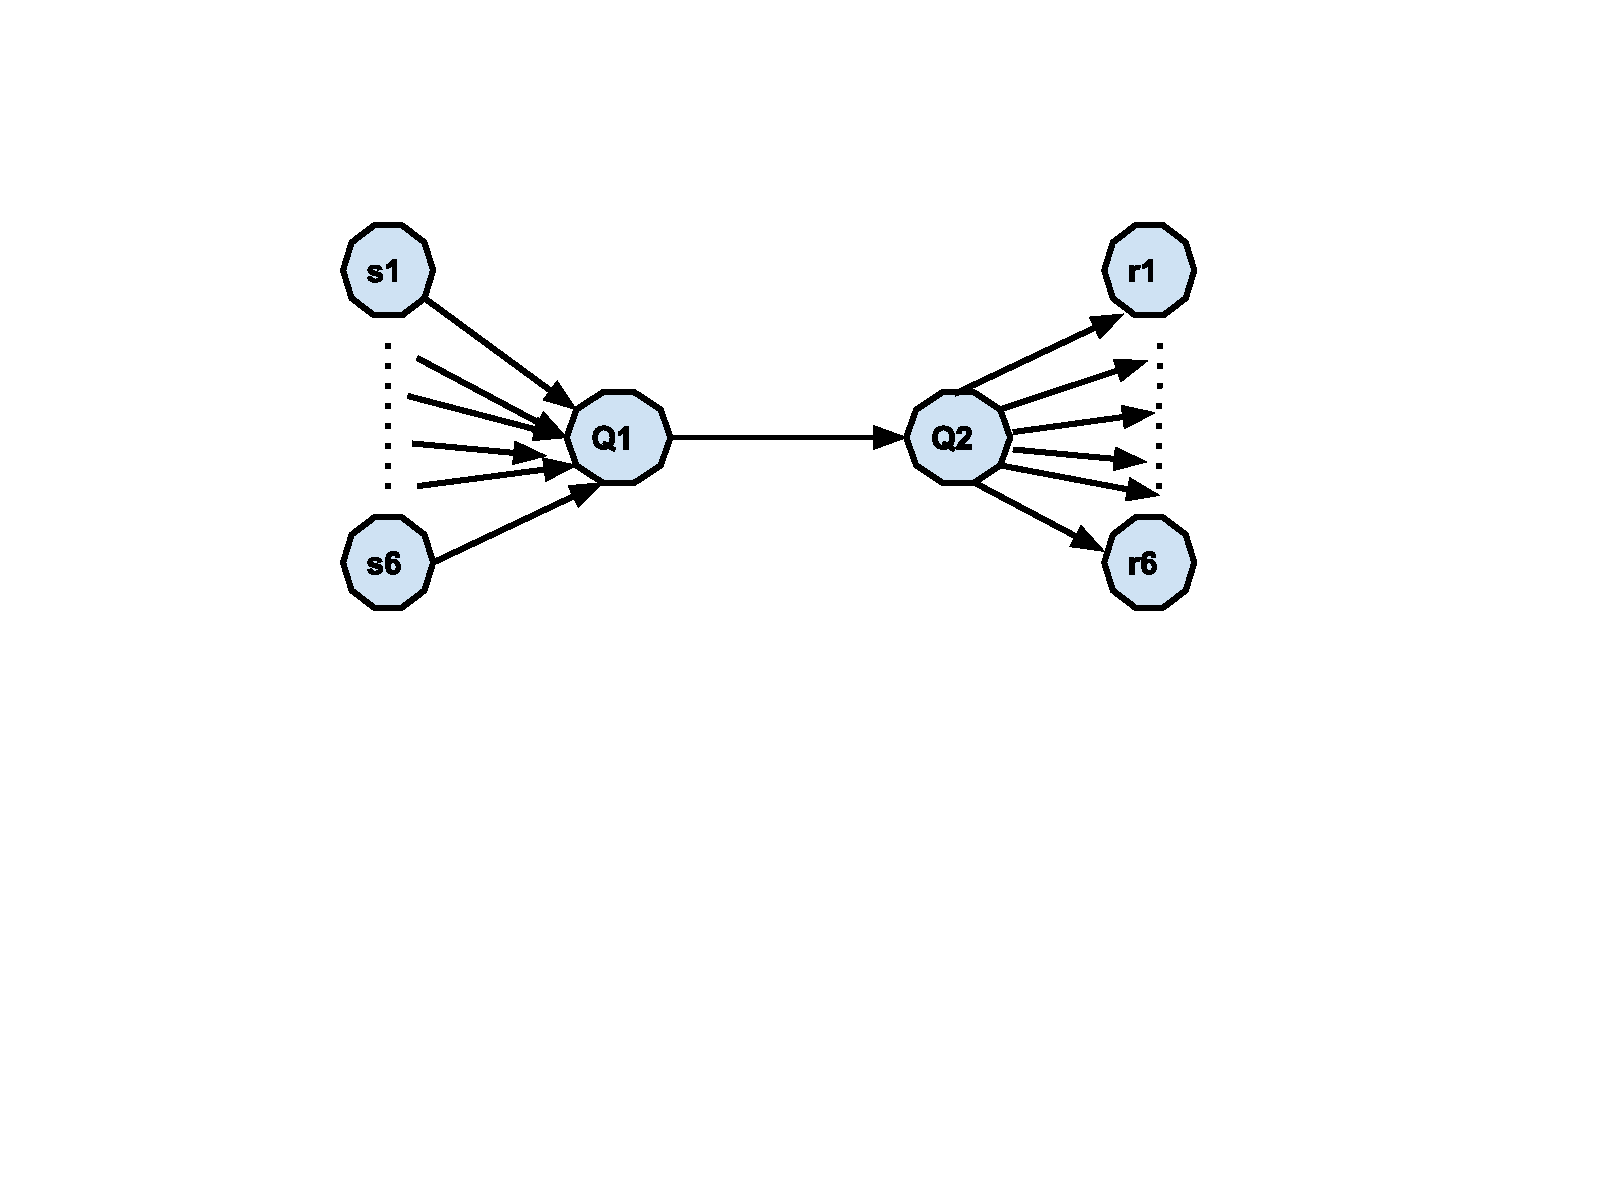
\includegraphics[width=10cm]{6layout.pdf}
\caption{Network topology}
\label{layout}
\end{figure}
Congestion occurs when the occupied queue length exceeds the threshold $T$ on the arrival of an incoming packet. To generate traces with congestion identifiers, we mark every packet as Congestion Experienced in the queue when queue length is greater than $T$. Typical NS2 TCP traces  \cite{TraceFormat} are collected for future data processing as in Figure \ref{NS2Format}. 

\begin{figure}
\centering
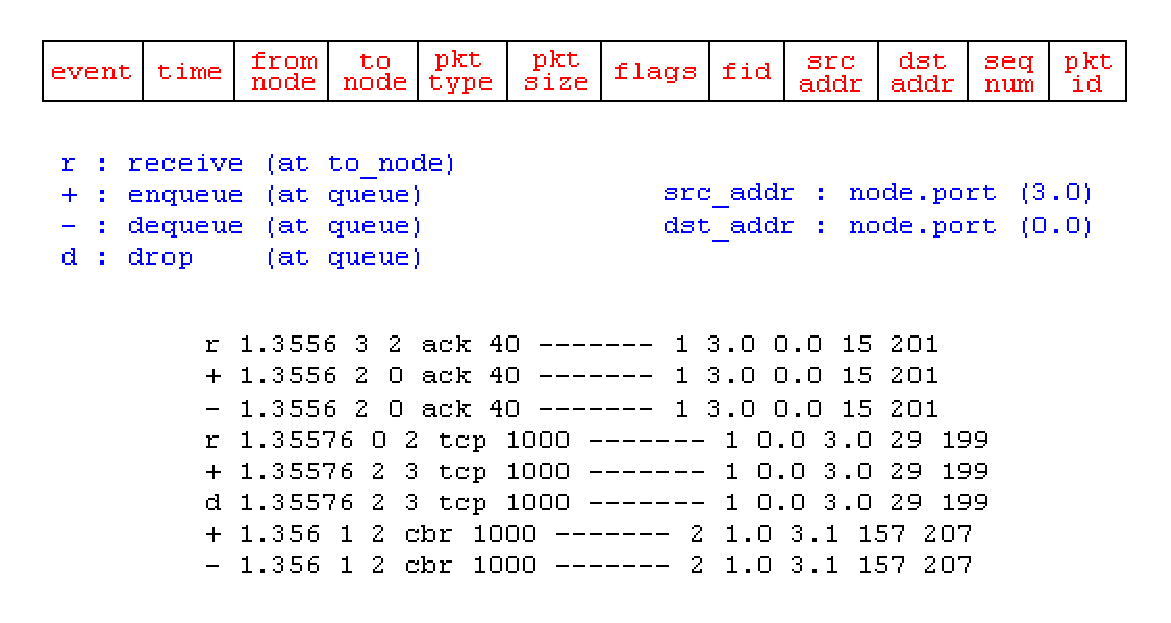
\includegraphics[width=10cm]{format.eps}
\caption{NS2 TCP trace format}
\label{NS2Format}
\end{figure}
From the trace format, we can identify the packet sending time, arriving time, packet size, unique ID, etc. Matching the packet unique ID, the RTT can be calculated from the packet sending time and the corresponding ACK receiving time. For each unique packet, if congestion occurs upon its arriving, the unique ID will be recorded to be Congestion Experienced.

\par The drop tail queue behavior is displayed as follows.
% Figure \ref{queuelengthCubic}
% and Figure \ref{queuelengthNewRenoVSUDP} are two different queue behavior patterns. 
Figure \ref{queuelengthCubic} shows queue changes when traffic sources are running Cubic TCP with competing UDP traffic. 
%while Fig. \ref{queuelengthNewRenoVSUDP} shows the case one part of traffic sources are running NewReno TCP with competing UDP traffic.
In this case, when the queue length is greater than $450$ packets, the incoming packets will be marked as Congestion Experienced.

%\begin{figure}
%\includegraphics[width=8cm]{queue.eps}
%\caption{Queue Length Dynamics (NewReno)}
%\label{queuelengthNewReno}
%\end{figure}
%\begin{figure}[!htb]\centering
%   \begin{subfigure}{0.49\textwidth}
%     \frame{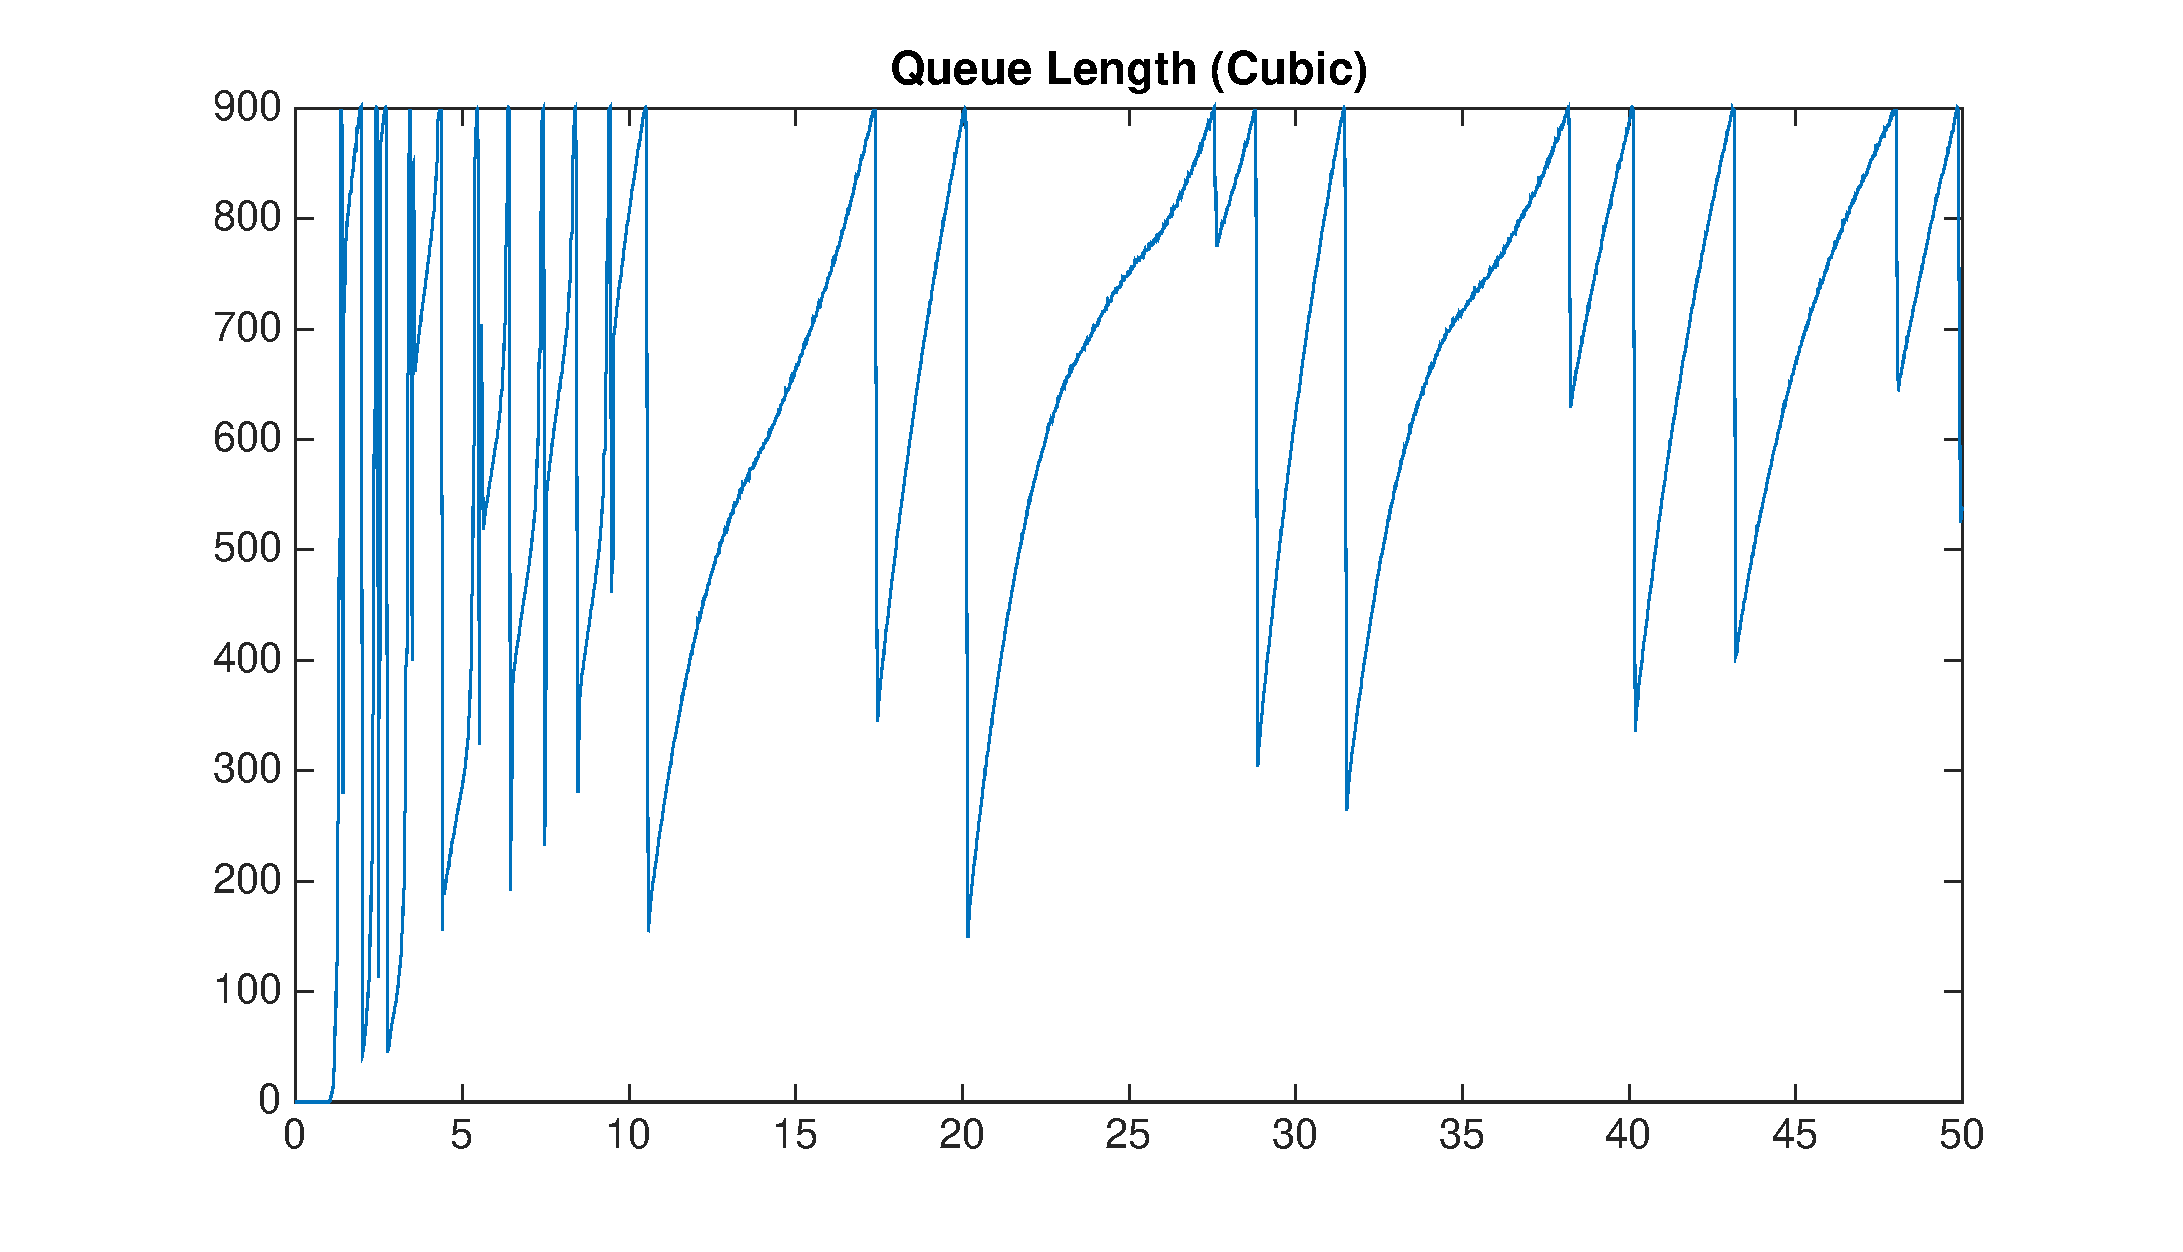
\includegraphics[width=6cm]{QueueLengthCubic.eps}}
%     \caption{Queue Length (Cubic)}
%\label{queuelengthCubic}
%   \end{subfigure}
%   \begin {subfigure}{0.49\textwidth}
%     \frame{\includegraphics[width=6cm]{QueueLengthNewRenoVSUDP.eps}}
%   \caption{Queue Length (NewReno VS UDP)}
%\label{queuelengthNewRenoVSUDP}
%   \end{subfigure}
%\end{figure}

\begin{figure}
\centering
\includegraphics[width=10cm]{QueueLengthCubic.eps}
\caption{Queue length dynamics (Cubic)}
\label{queuelengthCubic}
\end{figure}

%\begin{figure}
%\centering
%\includegraphics[width=10cm]{QueueLengthNewRenoVSUDP.eps}
%\caption{Queue Length Dynamics (NewReno VS UDP)}
%\label{queuelengthNewRenoVSUDP}
%\end{figure}

\subsection{Data Collection}
Without loss of generality, we simulated several different traffic scenarios to collect end-user data. We analyze the following scenarios: 
\begin{itemize}
    \item Scenario 1: All traffic sources are running TCP NewReno with stationary bottleneck link capacity.
    \item Scenario 2: All traffic sources are running TCP Cubic with stationary bottleneck link capacity.
    % \item Scenario 3: One half traffic sources are running TCP NewReno while the other half running TCP Cubic with stationary bottle link capacity.
    \item Scenario 3: One-half of the traffic sources is running TCP NewReno while the other half is running UDP with stationary bottleneck link capacity.
    \item Scenario 4: One-half of traffic sources is running TCP Cubic while the other half is running UDP with stationary bottleneck link capacity.
    \item Scenario 5: Repeat scenario 1 and 2 for a periodically On-Off bottleneck link.
\end{itemize}
The bottleneck link for those scenarios is link $Q1 \to Q2$. Detailed simulation parameters are shown in Table \ref{tab:simuPara}.

\par Data available from end-users includes packet sending time $t_{s}$ and ACK receiving time $t_{r}$. From these two timestamps, we can calculate packet sending interval $T_{s_{i}} = t_{s_{i}} - t_{s_{i-1}}$, ACK inter-arrival time $T_{r_{i}} = t_{r_{i}} - t_{r_{i-1}}$ and Round Trip Time (RTT) $RTT_{i} = t_{s_{i}} - t_{r_{i}}$. From the above three available time intervals, we develop 5 features that are used in the congestion prediction algorithm.
\begin{table}
\begin{center}
\caption {Simulation Parameters} \label{tab:simuPara}
\begin{tabular}{ |c|c| }
 \hline
 Access Link Capacity & 1Gbps  \\
 \hline
 Bottleneck Link Capacity & 1Gbps  \\
 \hline
 Access Link Delay & 5ms  \\
 \hline
 Bottleneck Link Delay & 10ms\\
 \hline
 Queue Capacity & Bandwidth-Delay Product\\
 \hline
\end{tabular}
\end{center}
\end{table}
\begin{itemize}
\item The sending time interval between two consecutive packets $T_{s_{i}}$ ($f_{1}$).
\item The receiving time interval between two consecutive ACKs $T_{r_{i}}$ ($f_{2}$).
\item An exponential weighted moving average (EWMA) of $T_{s_{i}}$ (send\_ewma, $f_{3}$).
\item An EWMA of $T_{r_{i}}$ (ack\_ewma, $f_{4}$).
\item The ratio between the most recent RTT and the minimum RTT during the entire connection period (rtt\_ratio, $f_{5}$).
\end{itemize}

These above five features construct the feature set to train the machine learning algorithm and predict congestions.

\subsection{Congestion Prediction}
\label{CongestionPredict}
\par Every sample of the data collected from above five scenarios includes five features and a congestion identifier: Virtual ECN (0 represents no congestion experienced, 1 represents congestion experienced). The problem to be solved is a binary classification problem \cite{alpaydin2014introduction}. We need to train an algorithm to classify the sample data into two categories: congestion experienced and no congestion experienced. First, we apply Logistic Regression \cite{hosmer2013applied}, a popular binary classification algorithm, to train the sample data and predict congestion. The area under receiver operating characteristic (ROC) curve \cite{hanley1982meaning} is $0.89$ as shown in Figure \ref{LRRoc}. The performance of Logistic Regression is good (area under ROC: $0.80 - 0.90$). The decision boundary is $ -2.32*f_{1} - 33.36*f_{2} - 12.65*f_{3} - 15.30*f_{4} + 2.03*f_{5} - 2.69 = 0$, where $f_{1}, f_{2}, f_{3}, f_{4}, f_{5}$ are the five corresponding features.
\begin{figure}
\centering
\includegraphics[width=10cm]{LRRoc.png}
\caption{ROC curve of the Logistic Regression classifier}
\label{LRRoc}
\end{figure}




\par Next, we applied the Decision Tree algorithm \cite{rokach2014data} and regulated the maximum depth of the tree to be $5$ and the minimum samples in each leaf node to be $10000$ to avoid overfitting. Figure \ref{DecisionTreeRoc} presents the ROC curve of the Decision Tree Classifier. The area under ROC curve is $0.98$. This indicates an excellent (area under ROC: $0.90 - 1$) prediction result. The feature importance is given as [$0.011703$, $0.00085$, $0.000000$, $0.03985$, $0.94760$] for [$T_{s_{i}}$, $T_{r_{i}}$, send\_ewma, receive\_ewma, rtt\_ratio], from which we can conclude that the rtt\_ratio is the most important feature to predict congestions. 
%\begin{figure}
%\centering
%\includegraphics[width=10cm]{DecisionTreeRoc.png}
%\caption{ROC curve of Decision Tree Classifier (max\_depth = 5, min\_samples\_leaf = 10000)}
%\label{DecisionTreeRoc}
%\end{figure}

\begin{figure}[!htb]\centering
   \begin{subfigure}{0.49\textwidth}
     \includegraphics[width=6cm]{DecisionTreeRoc.png}
\caption{max\_depth = 5, min\_samples\_leaf = 10000}
\label{DecisionTreeRoc}

   \end{subfigure}
   \begin {subfigure}{0.49\textwidth}
     \includegraphics[width=6cm]{DTRoc.png}
\caption{max\_depth = 3, min\_samples\_leaf = 100000}
\label{DTRoc}
   \end{subfigure}
   \caption{ROC curve of the Decision Tree classifier}
\label{fig:roc1}
\end{figure}
Furthermore, when we changed the maximum depth to $3$ and minimum samples of each leaf node to $100,000$, the ROC is displayed in Figure \ref{DTRoc}. The feature importance becomes [$0$, $0$, $0$, $0$, $1$]. This indicates the decision tree is doing the binary classification merely based on the rtt\_ratio. All other features do not contribute to the binary classification process at all. 
%\begin{figure}
%\centering
%\includegraphics[width=10cm]{DTRoc.png}
%\caption{ROC curve of Decision Tree Classifier (max\_depth = 3, min\_samples\_leaf = 100000)}
%\label{DTRoc}
%\end{figure}
The decision tree is shown in Figure \ref{DT}. In this figure, the first layer is classified by X[4]: rtt\_ratio. The cumulative density function (CDF) of the rtt\_ratio is given in Figure \ref{CDFrtt}. The blue line is the CDF curve of  the rtt\_ratio when congestion is experienced while the red line is the CDF curve when congestion is not experienced. Take rtt\_ratio $=1.2$ as an example, the probability of the rtt\_ratio to be less than $1.2$ is $82\%$ when there is no congestion. However, this probability is approximately $0\%$ when congestion is experienced. This is consistent with the result of feature importance generated from the Decision Tree algorithm. 

\begin{figure}
\centering
  \includegraphics[width=\textwidth,height=6cm]{tree.png}
  \caption{Decision Tree (max\_depth = 3, min\_samples\_leaf = 100000)}
  \label{DT}
\end{figure}

\begin{figure}[!htb]\centering
   \begin{subfigure}{0.49\textwidth}
     \frame{\includegraphics[width=6cm]{cdfrtt1.eps}}
\caption{CDF of rtt\_ratio with the same propagation delay}
\label{CDFrtt}

   \end{subfigure}
   \begin {subfigure}{0.49\textwidth}
     \frame{\includegraphics[width=6cm]{cdfrtt2.eps}}
\caption{CDF of rtt\_ratio with different propagation delays}
\label{CDFrttDiff}
   \end{subfigure}
\caption{CDF of rtt\_ratio}
\label{fig:cdf1}
\end{figure}



%\begin{figure}
%\centering
%\includegraphics[width=10cm]{cdfrtt1.eps}
%\caption{CDF of rtt\_ratio}
%\label{CDFrtt}
%\end{figure}

\par The above results are generated from a network with fixed propagation delay. To learn how this prediction algorithm works when network condition changes, we investigate Scenario 1 and 2 with variations of propagation delay. We simulate networks with access delay and queue capacity as in Table \ref{tab:varyRTT}.
\begin{table}
\begin{center}
\caption {Simulation Parameters} \label{tab:varyRTT}
\begin{tabular}{ |c|c| }
 \hline
 Access Link Delay & 5ms, 10ms, 20ms  \\
 \hline
 Bottleneck Link Delay & 10ms, 20ms, 40ms\\
 \hline
 Queue Capacity & Bandwidth-Delay Product\\
 \hline
\end{tabular}
\end{center}
\end{table}
The Logistic Regression algorithm generates ROC curve which is shown in Figure \ref{LRROCDiff}. The area under ROC curve is $0.65$, which indicates poor performance (area under ROC curve: $0.60-0.70$). The decision boundary is $ -0.47*f_{1} - 7.33*f_{2} - 0.35
*f_{3} - 1.41*f_{4} + 5.20*f_{5} - 5.54 = 0$. The coefficient of each feature follows the same pattern as before. The Decision Tree classifier is then applied to the collected dataset. The ROC curve is shown in Figure. \ref{DTROCDiff}. The area under the ROC curve is $0.70$, which is on the boundary of poor performance. The feature importance is [$0.000955787581$, $0.000389816495$, $0.00489484823$, $0.0636899225$, $0.930069625$]. This is consistent with the previous result that the rtt\_ratio is the most important feature. Those two figures indicate that when network condition changes, the predictability of congestion from the aforementioned five features decreases. Figure. \ref{CDFrttDiff} presents the CDF of the rtt\_ratio with different link propagation delays. In Figure \ref{CDFrttDiff}, two CDF curves overlap each other from $0\%$ to $30\%$. This means there are $30\%$ packets of the two different classes (congestion experienced and no congestion experienced) have the same $rtt\_ratio$ and cannot be classified by binary classifier. Comparing Figure \ref{CDFrtt} to Figure \ref{CDFrttDiff}, we find that bigger separation between the two CDF curves means higher prediction precision of the binary classifier. 
\begin{figure}[!htb]\centering
\begin{subfigure}{0.49\textwidth}
\includegraphics[width=7cm]{LRRocDiffProp.png}
\caption{ROC curve of Logistic Regression classifier with different propagation delays}
\label{LRROCDiff}
\end{subfigure}
\begin{subfigure}{0.49\textwidth}
\includegraphics[width=7cm]{DTRocDiffProp.png}
\caption{ROC curve of Decision Tree classifier with different propagation delays}
\label{DTROCDiff}
\end{subfigure}
\caption{ROC curves with different propagation delays}
\label{fig:roc2}
\end{figure}
%\begin{figure}
%\centering
%\includegraphics[width=10cm]{cdfrtt2.eps}
%\caption{CDF of rtt\_ratio with Different Propagation Delay}
%\label{CDFrttDiff}
%\end{figure}




\section{Chapter Summary}
\label{Conclusions and Future Work}
In this chapter, we propose a data-driven machine learning congestion detection algorithm. Datasets are collected using NS2 for a dumbbell topology with five different traffic scenarios. Five features are formatted from the end-user data. When the network condition is not changing, which means the propagation delay of each link is stable, our algorithm can detect congestion with high precision from those five features. In contrast, if the network condition changes, the algorithm fails to work. In both cases, the rtt\_ratio is the most important feature to predict congestions. The other four features are less useful when doing the binary classification. CDF curves of the rtt\_ratio explains our conclusion. For a stable network, a fast reacting congestion control algorithm can be designed based on our congestion detection algorithm for mmWave communication networks.

\chapter{Conclusion}\label{ch:conc}
\par In this thesis, we focus on studying the system performance in terms of outage probability and outage duration under correlated shadow fading, developing efficient ways to mitigate shadow fading, reduce outage and provide better Quality of Service (QoS) to users. Both physical layer and transportation layer performance are analyzed. For physical layer, downlink performance of single-cell model and multi-cell model are both investigated. Simulation results show that correlated shadow fading brings high outage probability and long outage duration. To mitigate shadow fading, cooperative communication and ultra-dense network are proposed. For transportation layer, legacy TCP are not performing well on mimic mmWave channel. A better scheme need to be developed. To develop a new proper TCP congestion control protocol for next generation networks, reduce congestion detection time is a key component. Based on this fact, we propose a fast end user congestion detection scheme which provides high precision when network topology does not change fast.
\section{Main Contributions}
\par The key contributions of this thesis are given as follows:
\begin{itemize}
\item In Chapter \ref{ch:CoopComm}, we investigate the correlated shadow fading problem in a single cell cellular network and shows that it could lead to correlated outage and long outage durations. A correlated outage field is presented. To mitigate shadow fading, relays can be deployed. The performance of three different relay deployments with different relay densities are studied. Theoretical analysis and simulations of outage performance are given to compare between different relay placement scenarios. Through these simulation, we showed that uniformly spaced relays perform better than the randomly spaced, due to the randomness of relay deployment. 
\item In Chapter \ref{ch:ExpSingleCell}, we investigated how shadow fading at different positions in a cellular network is correlated. To model spatially correlated shadow fading we divided the entire range of shadow fading into a finite number of intervals. A Markov chain model is then constructed, where each interval becomes a state of the Markov chain model. This model can be used to analyze the  outage behavior at the application layer. We demonstrated that a well designed Markov chain model with an appropriate number of states corresponding to the standard deviation of the shadow fading is indeed a powerful tool to study system performance. For a single-cell system, this Markov chain model is able to analyze the system performance because there only exist autocorrelation in this scenario. 
\item In Chapter \ref{ch:Multi}, we expand the work to investigate a multi-cell system performance given correlated shadow fading. Simulations are run to study the outage probability and outage duration distribution. First of all, the probability of two different BS layout: Grid Layout and Random Layout are investigated. We found that Grid Layout performs better than Random Layout. Secondly, outage probability given different BS densities and two different connecting strategies: Nearest BS and Strongest BS, are simulated. We conclude that connecting to Strongest BS will reduce the outage probability comparing with Nearest BS. Increasing BS density will not reduce outage probability when MU is connecting to the Strongest BS. However, when MU is connecting to the Nearest BS and the De-Correlation distance of correlated shadow fading is large enough, increasing BS density will reduce the outage probability. At last, we investigate system performance in terms of outage duration. The simulation results show that correlated shadow fading will result in long outage duration. Increasing BS density will efficiently reduce the percentage of long outage duration.
\item In Chapter \ref{ch:TCP5G}, we propose a data driven machine learning congestion detection algorithm. Datasets are collected using NS2 for a dumbbell model with five different traffic scenarios. Five features are formatted from end user data. When the network condition is not changing, which means the propagation delay of each link is stable, our algorithm can detect congestion with high precision from the five features. In contrast, if the network condition changes, the algorithm fails to work. In both cases, rtt\_ratio is the most important feature to predict congestion. Other four features are less useful when doing the binary classification. The area under ROC curve is consistent with the CDF of rtt\_ratio. For stable network, a fast reacting congestion control algorithm can be designed based on our congestion detection algorithm for 5G mmWave communication network.

\end{itemize}
\section{Future Work}
In the future, for next generation wireless communication network, mmWave channel will be used with high probability. Therefore, shadow fading will be a significant problem for next generation network. Algorithms to mitigate correlated shadow fading developed in this thesis can be directly applied to standard mmWave channel. To extend multi-cell model analysis, analysis of ultra dense network performance should will be a research direction. The fast end user congestion prediction algorithm can be used to design a fast reacting TCP congestion control algorithm. Real-time applications can be tested on top of the new designed transport layer protocol.
%\begin{appendices}
  \chapter{}\label{ch:app_1}
\section{Title of Appendix A}\label{app:app_1_A}

\chapter{}\label{ch:app_2}
\section{Title of Appendix B}\label{app:app_2_B}

\end{appendices}


\bibliographystyle{IEEEtran}
\bibliography{References}

\end{document}